\newpage
\section{\tkzClass{triangle} 类} %(fold)


变量 \tkzVar{triangle}{T} 保存一个用于存储三角形对象的表。它的使用是可选的：你可以自由选择其他变量名，但为了在各示例与文档中保持清晰和一致，推荐使用 \tkzVar{triangle}{T}。

\medskip
如果你定义自己的表，则必须手动初始化它。不过，若使用默认变量 \tkzVar{triangle}{T}，则调用 \code{init\_elements()} 函数时会自动清空并重置 \tkzVar{triangle}{T} 表。

\medskip
每个三角形对象都使用 \tkzMeth{triangle}{new} 方法创建，该方法以三个点为输入，并生成所有相关的几何属性。

\vspace{1em}

\subsection{创建三角形}
\label{sub:creating_a_triangle}

\tkzClass{triangle} 类用于由三个点定义三角形。
\textbf{注意。}三角形必须是非退化的。若两个顶点重合（在容差范围内），或三个顶点共线，构造函数会抛出错误。它会自动计算与该三角形相关的一系列几何属性。

\begin{mybox}
\begin{verbatim}
T.ABC = triangle:new(z.A, z.B, z.C)
\end{verbatim}
\end{mybox}

\texttt{简写：}

简写 \code{triangle(z.A, z.B, z.C)} 与之等价，且更常用：

\begin{mybox}
\begin{verbatim}
T.ABC = triangle(z.A, z.B, z.C)
\end{verbatim}
\end{mybox}


\subsection{三角形的属性} %(fold)

三角形对象使用 \tkzMeth{triangle}{new} 方法创建，例如：

\begin{center}
\code{T.ABC = triangle(z.A, z.B, z.C)}
\end{center}

有若干属性会被自动计算并存储：

\begin{itemize}
  \item \texttt{顶点：} 三个顶点可通过以下方式访问：
  \begin{center}
    \code{T.ABC.pa}, \code{T.ABC.pb}, \code{T.ABC.pc}
  \end{center}

  \item \texttt{边：} 边长为：
  \begin{align*}
    T.ABC.a &= \text{$BC$ 的长} \\
    T.ABC.b &= \text{$AC$ 的长} \\
    T.ABC.c &= \text{$AB$ 的长}
  \end{align*}

  \item \texttt{面积：} 面积用海伦公式计算：
  \[
    s = \frac{a + b + c}{2}, \quad \text{Area} = \sqrt{s(s - a)(s - b)(s - c)}
  \]
  该值存于 \code{T.ABC.area}。

  \item \texttt{周长：} 周长为各边长之和：
  \[
    P = a + b + c
  \]
  存于 \code{T.ABC.perimeter}。

  \item \texttt{角：} 内角 $\alpha$、$\beta$、$\gamma$（分别在 $A$、$B$、$C$ 处）用余弦定理计算：
  \[
  \cos(\alpha) = \frac{b^2 + c^2 - a^2}{2bc}, \quad
  \cos(\beta) = \frac{a^2 + c^2 - b^2}{2ac}, \quad
  \cos(\gamma) = \frac{a^2 + b^2 - c^2}{2ab}
  \]
  它们存于 \code{T.ABC.alpha}、\code{T.ABC.beta} 和 \code{T.ABC.gamma}。

  \item \texttt{中线、高与内角平分线的足：}
  \begin{itemize}
    \item |ma|, |mb|, |mc|：各边的中点。
    \item |ha|, |hb|, |hc|：高的垂足。
    \item |ia|, |ib|, |ic|：内角平分线的足。
  \end{itemize}
\end{itemize}

这些属性定义了三角形的基本几何性质，并被众多派生方法和作图所使用。


\bgroup
\catcode`_=12
\small
  \captionof{table}{三角形属性。}\label{triangle:attributes}
  \begin{tabular}{ll}
  \toprule
  \texttt{属性}     & \texttt{参考}\\
  \midrule
  \tkzAttr{triangle}{pa} &[\ref{ssub:triangle_attributes_points}]\\
  \tkzAttr{triangle}{pb} & 同上 \\
  \tkzAttr{triangle}{pc} & 同上 \\
  \tkzAttr{triangle}{type} & 'triangle' \\
  \tkzAttr{triangle}{circumcenter} &  [\ref{ssub:triangle_attributes_characteristic_points}]\\
  \tkzAttr{triangle}{centroid} & 同上  \\
  \tkzAttr{triangle}{incenter} & 同上 \\
  \tkzAttr{triangle}{orthocenter}  & 同上 \\
  \tkzAttr{triangle}{eulercenter} & 同上 \\
  \tkzAttr{triangle}{spiekercenter} & 同上； [\ref{ssub:triangle_attributes_characteristic_points}; \ref{ssub:example_apollonius_circle}]  \\
  \tkzAttr{triangle}{a}& [\ref{ssub:triangle_attributes_lengths}]  \\
  \tkzAttr{triangle}{b}& \\
  \tkzAttr{triangle}{c}&  \\
  \tkzAttr{triangle}{alpha}&[ \ref{ssub:triangle_attributes_angles}]\\
  \tkzAttr{triangle}{beta} & \\
  \tkzAttr{triangle}{gamma}& \\
  \tkzAttr{triangle}{alpha\_}&[ \ref{ssub:triangle_attributes_angles_objects}]\\
  \tkzAttr{triangle}{beta\_} & \\
  \tkzAttr{triangle}{gamma\_}& \\
  \tkzAttr{triangle}{ab}& [\ref{ssub:triangle_attributes_straight_lines}]\\
  \tkzAttr{triangle}{bc}&  \\
  \tkzAttr{triangle}{ca}&  \\
  \tkzAttr{triangle}{semiperimeter}& [\ref{ssub:triangle_attributes_lengths}] \\
  \tkzAttr{triangle}{area}&  \\
  \tkzAttr{triangle}{orientation}& [\ref{ssub:triangle_attributes_orientation}] \\
  \tkzAttr{triangle}{cross}& [\ref{ssub:triangle_attributes_cross}] \\
  \tkzAttr{triangle}{inradius}& [\ref{ssub:triangle_attributes_lengths}]\\
  \tkzAttr{triangle}{circumradius}& [\ref{ssub:triangle_attributes_lengths}] \\
  \tkzAttr{triangle}{ma/mb/mc}& [\ref{ssub:triangle_attributes_foot_median}]  \\
  \tkzAttr{triangle}{ha/hb/hc}& [\ref{ssub:triangle_attributes_foot_altitude}]\\
  \tkzAttr{triangle}{ia/ib/ic}& [\ref{ssub:triangle_attributes_foot_bisector}] \\
  \bottomrule %
  \end{tabular}
  \egroup



\subsubsection{三角形属性：定义点}
\label{ssub:triangle_attributes_points}

考虑三角形 $ABC$。我们想构造一个新三角形，其顶点分别是 $A$、$B$、$C$ 关于各自对边中点的反射点。

\medskip

为此，我们首先需要确定三角形 $ABC$ 各边的中点。最直接的方法是使用 \tkzMeth{triangle}{medial} 方法，它返回\textbf{中点三角形}，即由 $[BC]$、$[AC]$、$[AB]$ 的中点构成的三角形。

\medskip

一旦构造出这个中点三角形，其顶点即可通过标准属性访问：
\begin{center}
\code{T.medial.A}, \code{T.medial.B}, \code{T.medial.C}
\end{center}


或者，利用后者，\code{get()} 方法以一种方便的、与 Lua 兼容的语法一次性取回三个顶点。

\medskip

关于此方法的实际示例，参见文档中相应的 \code{tikzpicture} 示例。

\vspace{1em}

% 开发代码见 help.lua
\begin{minipage}{.5\textwidth-2cm}
\directlua{ init_elements()
  z.A = point(0, 0)
  z.B=  point(3, 0)
  z.C = point(1, 2)
  T.ABC = triangle(z.A, z.B, z.C)
  T.m = T.ABC:medial()
  z.ma, z.mb, z.mc = T.m.pa, T.m.pb, T.m.pc
  z.Ap = z.ma:symmetry(z.A)
  z.Bp = z.mb:symmetry(z.B)
  z.Cp = z.mc:symmetry(z.C)}
\begin{center}
  \begin{tikzpicture}[scale=.75]
   \tkzGetNodes
   \tkzDrawPolygons(A,B,C)
   \tkzDrawPoints(ma, mb, mc)
   \tkzDrawPoints(A, B, C, A', B', C')
   \tkzDrawSegments[dashed](A,A' B,B' C,C')
   \tkzDrawPolygons[red](A',B',C')
  \end{tikzpicture}
\end{center}
\end{minipage}
\begin{minipage}{.5\textwidth}
\begin{tkzexample}[code only]
\directlua{ init_elements()
  z.A = point(0, 0)
  z.B=  point(3, 0)
  z.C = point(1, 2)
  T.ABC = triangle(z.A, z.B, z.C)
  T.m = T.ABC:medial()
  z.ma, z.mb, z.mc = T.m.pa, T.m.pb, T.m.pc
  z.Ap = z.ma:symmetry(z.A)
  z.Bp = z.mb:symmetry(z.B)
  z.Cp = z.mc:symmetry(z.C)}
\end{tkzexample}
\end{minipage}

\subsubsection{三角形属性：特征点}
\label{ssub:triangle_attributes_characteristic_points}
该 \code{tikzpicture} 环境可在文档中查看。

\begin{tkzexample}[latex=.5\textwidth]
\directlua{
init_elements()
   z.A = point(0, 0)
   z.B = point(4, 0)
   z.C = point(1, 3)
   T.ABC = triangle(z.A, z.B, z.C)
   z.O = T.ABC.circumcenter
   z.I = T.ABC.incenter
   z.H = T.ABC.orthocenter
   z.G = T.ABC.centroid
   z.S = T.ABC.spiekercenter}
\begin{center}
  \begin{tikzpicture}
     \tkzGetNodes
     \tkzDrawPolygon(A,B,C)
     \tkzDrawPoints(A,B,C,O,G,I,H,S)
     \tkzDrawCircles(O,A)
     \tkzLabelPoints[below](A,B,O,G,I)
     \tkzLabelPoints[above](H,S)
     \tkzLabelPoints[above](C)
  \end{tikzpicture}
\end{center}
\end{tkzexample}



\subsubsection{三角形属性：角} %(fold)
\label{ssub:triangle_attributes_angles}
\noindent\textbf{数值度量。}
变量 \code{alpha}、\code{beta}、\code{gamma} 是\emph{数}
（以弧度计）。它们通过计算
\[
\alpha = \lvert \widehat(ZA,ZB,ZC)\rvert,\qquad
\beta  = \lvert \widehat(ZB,ZC,ZA)\rvert,\qquad
\gamma = \lvert \widehat(ZC,ZA,ZB)\rvert,
\]
得到，其中 \code{get\_angle\_} 返回一个有向角（可能为负，
取决于三个点的定向）。使用 \code{math.abs} 可保证
\code{alpha}、\code{beta}、\code{gamma} 表示\emph{无符号的}内角大小。

\begin{tkzexample}[latex=.5\textwidth-2cm]
\directlua{init_elements()
  z.A = point(0,0)
  z.B = point(5,0)
  z.C = point(2,3)
  T.ABC = triangle(z.A, z.B, z.C)
  S = T.ABC.alpha + T.ABC.beta + T.ABC.gamma}
\def\wangle#1{\tkzPN[2]{%
    \tkzUseLua{math.deg(T.ABC.#1)}}}
\begin{center}
  \begin{tikzpicture}
  \tkzGetNodes
  \tkzDrawPolygons(A,B,C)
  \tkzLabelAngle(B,A,C){$\wangle{alpha}^\circ$}
  \tkzLabelAngle(C,B,A){$\wangle{beta}^\circ$}
  \tkzLabelAngle(A,C,B){$\wangle{gamma}^\circ$}
  \end{tikzpicture}
\end{center}
三角之和为：\tkzUseLua{math.deg(S)}
\end{tkzexample}


\subsubsection{三角形属性：角对象} %(fold)
\label{ssub:triangle_attributes_angles_objects}
\noindent\texttt{角对象：}
变量 \code{alpha\_}、\code{beta\_}、\code{gamma\_} 是用
\code{angle:new(...)} 创建的 \tkzClass{angle} 类\emph{对象}。
它们存储定义该角的三点，并提供方法以取回角度
（弧度或度数），以及支持后续基于该角的几何运算或绘图。
\tkzMeth{triangle}{angle(i)} 方法 [见 \ref{ssub:method_triangle_angle}]
以与 \tkzMeth{triangle}{get(i)} 相同的编号给出这些对象；
这是推荐的做法。

\medskip
\noindent\texttt{注：}
函数 \code{get\_angle\_} 返回一个\emph{有向}角，
其正负取决于三个点的顺序。
其值通常在区间 $(-\pi,\pi]$ 内。
因此取绝对值便得到
（无向的）内角大小。

相比之下，\tkzClass{angle} 类的对象
可能会保留方向信息，
具体取决于其内部实现。
这一区别使我们既可以使用纯数值度量
（用于计算），
也可以使用完整的几何角对象
（用于作图和绘图）。

\texttt{示例：}

\parindent =0pt
\begin{tkzexample}[latex=.5\textwidth]
\directlua{
  init_elements()
  z.A = point(0, 0)
  z.C = point(3, 0)
  z.B = point(3, 2)
  T.ABC = triangle(z.A, z.B, z.C)
  A.A = T.ABC.alpha_
  A.B = T.ABC.beta_
  A.C = T.ABC.gamma_
  tex.print("A(value) = \\", A.A.value)
  tex.print('\\\\')
  tex.print("A(raw) = \\", A.A.raw)
  tex.print('\\\\')
  tex.print("A(deg) = \\", A.A.deg)}
\begin{center}
\begin{tikzpicture}
  \tkzGetNodes
  \tkzDrawPolygon(A,B,C)
  \tkzDrawPoints(A,B,C)
  \tkzLabelPoints(A,C)
  \tkzLabelPoints[above](B)
\end{tikzpicture}
\end{center}
\end{tkzexample}

\subsubsection{三角形属性：长度}
\label{ssub:triangle_attributes_lengths}

你可以访问各种长度，尤其是边长，方式如下：
\begin{mybox}
\begin{tkzexample}[code only]
  T.ABC = triangle(z.A, z.B, z.C)
  -- T.ABC.a, T.ABC.b and T.ABC.c are the lengths of the sides opposite A, B and C
  p = T.ABC.a + T.ABC.b + T.ABC.c -- perimeter of T.ABC
  -- Other accessible lengths
  s = T.ABC.semiperimeter
  ri = T.ABC.inradius
  R = T.ABC.circumradius
  A = T.ABC.area
\end{tkzexample}
\end{mybox}

\subsubsection{三角形属性：直线}
\label{ssub:triangle_attributes_straight_lines}

与三角形各边和直线相关的若干属性可简化代码编写、提高可读性。

\medskip

考虑三角形 $ABC$。假设你想用到边 $[BC]$ 的中点（也可视为从 $A$ 引出的中线的垂足）。在 Lua 中构造这个中点有多种方法，但最简洁的是：

\begin{center}
\code{T.bc.mid}
\end{center}


其中：
\begin{itemize}
  \item \code{T.ABC.bc} 是表示直线 $(BC)$ 的属性，
  \item 它等价于写 \code{L.BC = line(z.B, z.C)}，
  \item 但若已有一个定义为 \code{T.ABC} 的三角形对象，你可以简单地写：
  \begin{center}
  \code{L.BC = T.ABC.bc}
  \end{center}
\end{itemize}

\medskip

在用三角形的边来处理中线、高、角平分线或投影的脚本中，这种方法既省时又省空间。

\vspace{1em}

\begin{tkzexample}[latex=.5\textwidth]
\directlua{
  z.A = point(0, 0)
  z.B = point(5, 0)
  z.C = point(2, 3)
  T.ABC = triangle(z.A, z.B, z.C)
  z.M = T.ABC.bc.mid
  L.AM = line(z.A, z.M)
  z.Q = L.AM.mid }
\begin{tikzpicture}
  \tkzGetNodes
  \tkzDrawPolygon(A,B,C)
  \tkzDrawLine[add = 0 and 1](A,Q)
  \tkzDrawPoints(A,B,C,M,Q)
  \tkzLabelPoints(A,B)
  \tkzLabelPoints[above](C,M,Q)
  \end{tikzpicture}
\end{tkzexample}

\subsubsection{三角形属性：定向}
\label{ssub:triangle_attributes_orientation}
三角形的 \tkzAttr{triangle}{orientation} 属性表示其顶点的定向。
当顶点按逆时针顺序排列时为正，
按顺时针排列时为负，
三点共线时为零。
在几何上，该值对应于三角形有向面积的符号。

\begin{tkzexample}[latex=.5\textwidth]
\directlua{
  init_elements()
  z.A = point(0, 0)
  z.B = point(2, 0)
  z.C = point(1, 1)
  T.ABC = triangle(z.A, z.B, z.C)
  tex.print("orientation =\\ ",
            T.ABC.orientation)}
\begin{center}
\begin{tikzpicture}[scale = 3]
  \tkzGetNodes
  \tkzDrawPolygon(A,B,C)
  \tkzDrawPoints(A,B,C)
  \tkzLabelPoints(A,B)
  \tkzLabelPoints[above](C)
\end{tikzpicture}
\end{center}
\end{tkzexample}

\subsubsection{三角形属性：叉积}
\label{ssub:triangle_attributes_cross}
在 \tkzNamePack{tkz-elements} 中，运算符 \verb|^| 表示向量的二维
叉积。
对于三个点 $A$、$B$、$C$，表达式

$(B - A)$\ \verb|^|\ $(C - A)$

返回一个标量值。
它的符号表示向量 $\overrightarrow{AB}$ 与 $\overrightarrow{AC}$ 的相对方向：
正值对应逆时针旋转，
负值对应顺时针旋转，
零值表示共线。

\begin{tkzexample}[latex=.5\textwidth]
\directlua{
  init_elements()
  z.A = point(0, 0)
  z.B = point(1, 1)
  z.C = point(2, 0)
  T.ABC = triangle(z.A, z.B, z.C)
  local cross = (z.B - z.A) ^ (z.C - z.A)
  tex.print("cross =\\ ", cross)}
\begin{center}
\begin{tikzpicture}[scale = 3]
  \tkzGetNodes
  \tkzDrawPolygon(A,B,C)
  \tkzDrawPoints(A,B,C)
  \tkzLabelPoints(A,C)
  \tkzLabelPoints[above](B)
\end{tikzpicture}
\end{center}
\end{tkzexample}

\subsubsection{三角形属性：中线足}
\label{ssub:triangle_attributes_foot_median}

\begin{tkzexample}[latex=.5\textwidth]
\directlua{
init_elements()
   z.A = point(0, 0)
   z.B = point(4, 0)
   z.C = point(1, 3)
   T.ABC = triangle(z.A, z.B, z.C)
   z.M_a = T.ABC.ma
   z.M_b = T.ABC.mb
   z.M_c = T.ABC.mc
   z.G = T.ABC.centroid}
\begin{center}
  \begin{tikzpicture}
     \tkzGetNodes
     \tkzDrawPolygon(A,B,C)
     \tkzDrawSegments[dashed](A,M_a B,M_b C,M_c)
     \tkzDrawPoints(A,B,C,M_a,M_b,M_c,G)
     \tkzLabelPoints[below](A,B,M_c,G)
     \tkzLabelPoints[left](M_b)
     \tkzLabelPoints[right](M_a)
     \tkzLabelPoints[above](C)
  \end{tikzpicture}
\end{center}
\end{tkzexample}

\subsubsection{三角形属性：高的垂足}
\label{ssub:triangle_attributes_foot_altitude}

\begin{tkzexample}[latex=.5\textwidth]
\directlua{
init_elements()
   z.A = point(0, 0)
   z.B = point(4, 0)
   z.C = point(1, 3)
   T.ABC = triangle(z.A, z.B, z.C)
   z.H_a = T.ABC.ha
   z.H_b = T.ABC.hb
   z.H_c = T.ABC.hc
   z.H = T.ABC.orthocenter}
\begin{center}
  \begin{tikzpicture}
     \tkzGetNodes
     \tkzDrawPolygon(A,B,C)
     \tkzDrawSegments[dashed](A,H_a B,H_b C,H_c)
     \tkzDrawPoints(A,B,C,H_a,H_b,H_c,H)
     \tkzLabelPoints[below](A,B,H_c,H)
     \tkzLabelPoints[left](H_b)
     \tkzLabelPoints[right](H_a)
     \tkzLabelPoints[above](C)
  \end{tikzpicture}
\end{center}
\end{tkzexample}

\subsubsection{三角形属性：内角平分线足}
\label{ssub:triangle_attributes_foot_bisector}

\begin{tkzexample}[latex=.4\textwidth]
\directlua{
init_elements()
   z.A = point(0, 0)
   z.B = point(4, 0)
   z.C = point(1, 3)
   T.ABC = triangle(z.A, z.B, z.C)
   z.I_a = T.ABC.ia
   z.I_b = T.ABC.ib
   z.I_c = T.ABC.ic
   z.I = T.ABC.incenter
   z.ta,z.tb,z.tc = T.ABC:projections(z.I)}
\begin{center}
\begin{tikzpicture}
 \tkzGetNodes
 \tkzDrawPolygon(A,B,C)
 \tkzDrawSegments[dashed](A,I_a B,I_b C,I_c)
 \tkzDrawCircle(I,ta)
 \tkzDrawPoints(A,B,C,I_a,I_b,I_c,I,ta,tb,tc)
 \tkzLabelPoints[below](A,B,I_c,I)
 \tkzLabelPoints[left](I_b)
 \tkzLabelPoints[right](I_a)
 \tkzLabelPoints[above](C)
\end{tikzpicture}
\end{center}
\end{tkzexample}

\subsection{triangle 类的方法} %(fold)


\begin{minipage}{\textwidth}
\bgroup
\catcode`_=12
\small
\captionof{table}{triangle 的方法。}\label{triangle:methods}
\begin{tabular}{ll}
\toprule
\texttt{构造函数} & \texttt{参考}      \\
\midrule
\tkzMeth{triangle}{new}(a, b ,c) &  [\ref{sub:creating_a_triangle}; \ref{ssub:method_triangle_new_pt_pt_pt}]\\
\midrule

\texttt{返回布尔值的方法}&\\
\midrule
\tkzMeth{triangle}{check\_isosceles(<EPS>)} & [\ref{ssub:method_triangle_check_isosceles}]\\
\tkzMeth{triangle}{in\_out(pt)}  & [\ref{ssub:_triangle_in__out_pt}]\\
\tkzMeth{triangle}{on\_triangle(pt)}  & [\ref{ssub:method_triangle_on_triangle}]\\
\tkzMeth{triangle}{check\_equilateral()}&[\ref{ssub:_triangle_check__equilateral}] \\
\tkzMeth{triangle}{check\_acutangle()} &[\ref{ssub:_triangle_check__acutangle}] \\
\midrule

\texttt{返回字符串的方法} &\\
\midrule
\tkzMeth{triangle}{position(pt, EPS)}  & [\ref{ssub:method_triangle_position}]\\
\midrule
\texttt{返回实数的方法} &\\
\midrule
\tkzMeth{triangle}{parameter(pt)} & [\ref{ssub:method_triangle_parameter}]\\
\tkzMeth{triangle}{barycentric\_coordinates(pt)}& [\ref{ssub:_triangle_barycentric__coordinates_pt}]\\
\tkzMeth{triangle}{trilinear\_coordinates(pt)} & [\ref{ssub:triangle_trilinear_coordinates_pt}]\\
\tkzMeth{triangle}{get\_angle(arg)} & [\ref{ssub:method_triangle_get_angle}] \\
\tkzMeth{triangle}{angle(i)}（\tkzClass{angle} 类对象） & [\ref{ssub:method_triangle_angle}] \\
\tkzMeth{triangle}{trilinear\_to\_d} & \ref{ssub:triangle_trilinear_to_d}\\
\midrule
\texttt{返回点的方法} &\\
\midrule
\tkzMeth{triangle}{brocard\_midpoint()} & [\ref{ssub:method_triangle_brocard_midpoint}]\\
\tkzMeth{triangle}{soddy\_points()} & [\ref{ssub:method_triangle_soddy_points}]\\
\tkzMeth{triangle}{conway\_center()} & [\ref{ssub:method_triangle_conway_center}]\\
\tkzMeth{triangle}{the\_apollonius\_center()} & [\ref{ssub:method_triangle_the_apollonius_center}]\\
\tkzMeth{triangle}{get(arg)} & [\ref{ssub:method_triangle_get}]\\
\tkzMeth{triangle}{point(r)} & [\ref{ssub:method_triangle_point_r}]\\
\tkzMeth{triangle}{random(<'inside'>)} & [\ref{ssub:method_triangle_random_inside}]\\
\tkzMeth{triangle}{barycentric(ka,kb,kc)} &\ref{ssub:_triangle_barycentric_ka_kb_kc}\\
\tkzMeth{triangle}{base(u,v)} & [\ref{ssub:method_triangle_base}] \\
\tkzMeth{triangle}{trilinear(u,v,w)}  & [\ref{ssub:method_triangle_trilinear_x_y_z}] \\
\tkzMeth{triangle}{lemoine\_point()} &  [\ref{ssub:method_line_isosceles}]\\
\tkzMeth{triangle}{symmedian\_point()} & [\ref{ssub:method_triangle_symmedial}] \\
\tkzMeth{triangle}{lemoine\_point()}  &  [\ref{ssub:method_triangle_symmedial}] \\
\tkzMeth{triangle}{bevan\_point()}  &  [\ref{ssub:method_imeth_triangle_bevan_point}; \ref{ssub:methods_triangle_bevan_circle}]\\
\tkzMeth{triangle}{mittenpunkt\_point()} &  [\ref{ssub:method_triangle_mittenpunkt}]\\
\tkzMeth{triangle}{gergonne\_point()} & [\ref{ssub:gergonne_point}]\\
\tkzMeth{triangle}{nagel\_point()} & [\ref{ssub:method_triangle_nagel__point}]\\
\tkzMeth{triangle}{feuerbach\_point()} & [\ref{ssub:method_point_feuerbach}]\\
\tkzMeth{triangle}{spieker\_center()} & [\ref{ssub:method_triangle_spieker_center}]\\
\tkzMeth{triangle}{projections(p)}  & [\ref{ssub:method_triangle_projections_pt}]\\
\tkzMeth{triangle}{reflections(p)}  & [\ref{ssub:method_triangle_reflections_pt}]\\
\tkzMeth{triangle}{euler\_points()} &  [\ref{ssub:method_triangle_euler__points}] \\
\tkzMeth{triangle}{medial\_points()} &  [\ref{ssub:method_triangle_special_points}] \\
\tkzMeth{triangle}{orthic\_points()} &  [\ref{ssub:method_triangle_special_points}] \\
\tkzMeth{triangle}{tangential\_points()} &  [\ref{ssub:method_triangle_special_points}] \\
\tkzMeth{triangle}{nine\_points()} &  [\ref{ssub:method_triangle_nine__points}] \\
\tkzMeth{triangle}{taylor\_points()} & 参见 [\ref{ssub:method_triangle_taylor__circle}]\\
\tkzMeth{triangle}{parallelogram()} & [\ref{ssub:director_circle}]\\
\tkzMeth{triangle}{kimberling(n)}  & 参见 [\ref{ssub:method_triangle_kimberling_n}]\\
\tkzMeth{triangle}{isogonal(p)}  & 参见 [\ref{ssub:method_triangle_isogonal}]\\
\tkzMeth{triangle}{macbeath\_point()} & 参见 [\ref{ssub:method_triangle_macbeath_point}]\\
\tkzMeth{triangle}{poncelet\_point(p)} & 参见 [\ref{ssub:method_triangle_poncelet_point}]\\
\tkzMeth{triangle}{orthopole(L)}  & 参见 [\ref{ssub:method_triangle_orthopole}]\\
\tkzMeth{triangle}{first\_fermat\_point()}  &
 参见 [\ref{ssub:method_triangle_first_fermat_point}] \\
\tkzMeth{triangle}{second\_fermat\_point()}  &
参见 [\ref{ssub:method_triangle_second__fermat__point}] \\
\tkzMeth{triangle}{lamoen\_points()}  &
参见 [\ref{ssub:method_triangle_lamoen_points}]\\
\tkzMeth{triangle}{soddy\_center()}  &
参见 [\ref{ssub:method_triangle_soddy_center}] \\
\tkzMeth{triangle}{conway\_points()}  &
参见 [\ref{ssub:method_triangle_conway_points}] \\
\tkzMeth{triangle}{kenmotu\_point()}  &
参见 [\ref{ssub:_triangle_kenmotu__point}] \\
\tkzMeth{triangle}{orthic\_axis\_points()}  &
参见 [ \ref{ssub:method_triangle_orthic}; \ref{ssub:method_triangle_orthic_axis_points}]\\
\tkzMeth{triangle}{isodynamic\_points()} & [\ref{ssub:isodynamic_points}] \\
\tkzMeth{triangle}{apollonius\_point()} & [\ref{ssub:apollonius_point}] \\
\tkzMeth{triangle}{cevian\_point()} & [\ref{ssub:cevian_point}] \\
\bottomrule
\end{tabular}
\egroup
\end{minipage}



\begin{minipage}{\textwidth}
\bgroup
  \catcode`_=12
  \small
  \captionof{table}{triangle 的方法。}
  \begin{tabular}{ll}
  \toprule
  \texttt{方法} & \texttt{参考}      \\
  \midrule

\texttt{返回直线的方法} &\\
\midrule
\tkzMeth{triangle}{trisector(arg)} & [\ref{ssub:method_triangle_trisector}]\\
\tkzMeth{triangle}{soddy\_line()} & [\ref{ssub:method_triangle_soddy_line}]\\
\tkzMeth{triangle}{altitude(arg) } & [\ref{ssub:method_triangle_altitude}]\\
\tkzMeth{triangle}{bisector(arg) }  &  [\ref{ssub:method_triangle_bisector}]\\
\tkzMeth{triangle}{bisector\_ext(arg) } & [\ref{ssub:method_triangle_bisector_ext}]\\
\tkzMeth{triangle}{mediator(arg)} & [\ref{ssub:triangle_mediator}]\\
\tkzMeth{triangle}{symmedian\_line(arg)} & [\ref{ssub:method_imeth_triangle_symmedian__line}
; \ref{ssub:method_triangle_symmedial} ; \ref{ssub:method_line_isosceles}]\\
\tkzMeth{triangle}{euler\_line() } &[\ref{ssub:euler_line}]\\
\tkzMeth{triangle}{antiparallel(pt,n)} & [\ref{antiparallel};\ref{sub:antiparallel_through_lemoine_point}]\\
\tkzMeth{triangle}{steiner\_line(pt)} &[\ref{ssub:method_triangle_steiner__line}] \\
\tkzMeth{triangle}{simson\_line(pt)} &[\ref{ssub:method_triangle_simson__line}] \\
\tkzMeth{triangle}{lemoine\_axis()} &[\ref{ssub:method_triangle_lemoine__line}] \\
\tkzMeth{triangle}{brocard\_axis()} &[\ref{ssub:method_triangle_brocard__axis}] \\
\tkzMeth{triangle}{fermat\_axis()}  & \\
\tkzMeth{triangle}{orthic\_axis()}  & 参见 [\ref{ssub:method_triangle_orthic_axis}]\\
\bottomrule
\end{tabular}
\egroup
\end{minipage}




\newpage
\bgroup
\catcode`_=12
\small
\begin{minipage}{\textwidth}
\begin{tabular}{ll}
\toprule
\texttt{方法} & \textbf{说明}     \\
\midrule
\texttt{返回圆的方法} &\\
\midrule
\tkzMeth{triangle}{thebault\_circles(pt)} & [\ref{ssub:method_triangle_thebault_circles}]\\
\tkzMeth{triangle}{the\_apollonius\_circle()} & [\ref{ssub:method_triangle_the_apollonius_circle}]\\
\tkzMeth{triangle}{euler\_circle()} &   [\ref{ssub:method_triangle_euler_circle}]\\
\tkzMeth{triangle}{circum\_circle()}  & [\ref{ssub:method_triangle_circum_circle}] \\
\tkzMeth{triangle}{in\_circle()}  &[\ref{ssub:method_triangle_in_circle}]\\
\tkzMeth{triangle}{ex\_circle(n)}  & [\ref{ssub:method_triangle_ex__circle}]\\
\tkzMeth{triangle}{first\_lemoine\_circle()} & [\ref{ssub:method_triangle_first_lemoine_circle}] \\
\tkzMeth{triangle}{second\_lemoine\_circle()}&  \ref{sub:antiparallel_through_lemoine_point}]\\
\tkzMeth{triangle}{spieker\_circle()} &  [\ref{ssub:method_triangle_spieker__circle}]\\
\tkzMeth{triangle}{bevan\_circle()}  & [\ref{ssub:methods_triangle_bevan_circle}]\\
\tkzMeth{triangle}{cevian\_circle()} &  [\ref{ssub:_triangle_cevian__circle_pt}
; \ref{ssub:method_triangle_cevian}]\\
\tkzMeth{triangle}{symmedial\_circle()}  & [\ref{ssub:method_triangle_symmedial_circ}; \ref{ssub:method_triangle_symmedial}]\\
\tkzMeth{triangle}{pedal\_circle()} &  [\ref{ssub:method_triangle_pedal}]\\
\tkzMeth{triangle}{conway\_circle()} &  [\ref{ssub:method_triangle_conway}]\\
\tkzMeth{triangle}{taylor\_circle()} &  [\ref{ssub:method_triangle_taylor__circle}]\\
\tkzMeth{triangle}{kenmotu\_circle()}  & [\ref{ssub:kenmotu_circle}]\\
\tkzMeth{triangle}{c\_c(pt)}  &  [\ref{ssub:method_triangle_c_c}]\\
\tkzMeth{triangle}{thebault(pt)}  &  [\ref{ssub:method_triangle_c_c}]\\
\tkzMeth{triangle}{mixtilinear\_incircle(arg)}  &  [\ref{ssub:method_triangle_mixti}]\\
\tkzMeth{triangle}{three\_tangent\_circles} &  [\ref{ssub:method_triangle_three_tgt_c}]\\
\tkzMeth{triangle}{adams\_circle()}  & [\ref{ssub:method_triangle_adams_circle}]\\
\tkzMeth{triangle}{lamoen\_circle()}  &
  参见 [\ref{ssub:method_triangle_lamoen_points}] \\
\tkzMeth{triangle}{soddy\_circle()}  &
  参见 [\ref{ssub:method_triangle_soddy_circle}] \\
\tkzMeth{triangle}{three\_apollonius\_circles()}  &
  参见 [\ref{ssub:three_apollonius_circles}] \\
\tkzMeth{triangle}{apollonius\_circle(side, EPS)}  &
  参见 [\ref{ssub:apollonius_circle}] \\
\tkzMeth{triangle}{feuerbach\_apollonius\_k181(EPS)}  &
  参见 [\ref{ssub:feuerbach_apollonius_k181}] \\
\tkzMeth{triangle}{feuerbach\_apollonius(EPS)}  &
  参见 [\ref{ssub:feuerbach_apollonius}] \\
\midrule

\texttt{返回三角形的方法} &\\
\midrule
\tkzMeth{triangle}{morley()} & [\ref{ssub:method_triangle_morley}]\\
\tkzMeth{triangle}{napoleon(<"swap">)} & [\ref{ssub:method_triangle_napoleon}]\\
\tkzMeth{triangle}{orthic()}   & [\ref{ssub:method_triangle_altitude}]   \\
\tkzMeth{triangle}{medial()} &  [\ref{ssub:method_triangle_medial} ; \ref{ssub:method_triangle_symmedial}]\\
\tkzMeth{triangle}{incentral()}  &[\ref{ssub:method_incentral}] \\
\tkzMeth{triangle}{excentral()}  &[\ref{ssub:method_triangle_excentral}; \ref{ssub:method_triangle_feuerbach}]  \\
\tkzMeth{triangle}{extouch()}   &[\ref{ssub:method_triangle_extouch}] \\
\tkzMeth{triangle}{intouch() }   &[\ref{ssub:method_triangle_intouch}; \ref{ssub:gergonne_point}]\\
\tkzMeth{triangle}{contact() } &  contact = intouch； [
\ref{ssub:gergonne_point}] \\
\tkzMeth{triangle}{tangential()} &[\ref{ssub:method_triangle_tangential}]\\
\tkzMeth{triangle}{anti() }&  反补三角形 [\ref{ssub:method_triangle_anti}]  \\
\tkzMeth{triangle}{cevian(pt)} & [\ref{ssub:method_triangle_cevian}] \\
\tkzMeth{triangle}{pedal(pt)} &[\ref{ssub:method_triangle_pedal}]\\
\tkzMeth{triangle}{symmedial()}  &[\ref{ssub:method_triangle_symmedial}] \\
\tkzMeth{triangle}{euler()} & [\ref{ssub:method_triangle_euler}; \ref{ssub:method_triangle_euler__points}] \\
\tkzMeth{triangle}{lemoine()} &[\ref{ssub:method_triangle_lemoine}] \\
\tkzMeth{triangle}{macbeath()}  & 参见 [\ref{ssub:method_triangle_macbeath}]\\
\tkzMeth{triangle}{circumcevian()}  & 参见 [  \ref{ssub:method_triangle_circumcevian}]\\


\midrule
\texttt{返回圆锥曲线的方法} &\\
\tkzMeth{triangle}{kiepert\_parabola()} & [\ref{ssub:method_triangle_kiepert_parabola}] \\
\tkzMeth{triangle}{kiepert\_hyperbola()} & [\ref{ssub:method_triangle_kiepert__hyperbola}] \\

\tkzMeth{triangle}{ellipse\_inscribed(...)}  & [\ref{ssub:ellipse_inscribed}]\\
\tkzMeth{triangle}{steiner\_inellipse()}& [ \ref{ssub:steiner_inellipse_and_circumellipse}] \\
\tkzMeth{triangle}{steiner\_circumellipse()} & [ \ref{ssub:steiner_inellipse_and_circumellipse}] \\
\tkzMeth{triangle}{euler\_ellipse()}  & [\ref{ssub:euler_ellipse}]\\
\tkzMeth{triangle}{lemoine\_inellipse()} & [\ref{ssub:method_triangle_lemoine_inellipse}]\\
\tkzMeth{triangle}{brocard\_inellipse()}  & [\ref{ssub:method_triangle_brocard__inellipse}]\\
\tkzMeth{triangle}{macbeath\_inellipse()}  & [\ref{ssub:method_triangle_macbeath__inellipse}]\\
\tkzMeth{triangle}{mandart\_inellipse()}  & [\ref{ssub:method_triangle_mandart__inellipse}]\\
\tkzMeth{triangle}{orthic\_inellipse()}  & [\ref{ssub:method_triangle_orthic__inellipse}]\\
\tkzMeth{triangle}{projection()}  & [见 \ref{ssub:method_triangle_projection}]\\
\tkzMeth{triangle}{reflection()}  & [见 \ref{ssub:method_triangle_reflection}; \ref{ssub:method_triangle_simson__line}; \ref{ssub:method_yiu_circles}]\\
\midrule
\texttt{返回正方形的方法} &\\
\tkzMeth{triangle}{square\_inscribed()}  &  [示例(\ref{ssub:method_triangle_square__inscribed}]\\
\bottomrule
\end{tabular}
 \end{minipage}
\egroup



\subsubsection{方法 \tkzMeth{triangle}{new(pt, pt, pt)}}
\label{ssub:method_triangle_new_pt_pt_pt}

该方法由三个给定点创建一个三角形对象，这三个点将作为其顶点。

\medskip

它被广泛使用，出现在大多数示例中。语法为：

\begin{center}
\code{T.ABC = triangle(z.A, z.B, z.C)}
\end{center}


所得对象包含许多预先计算好的属性，例如：
\begin{itemize}
  \item \code{T.ABC.A}, \code{T.ABC.B}, \code{T.ABC.C} —— 顶点，
  \item \code{T.a}, \code{T.b}, \code{T.ABC.c} —— 边长，
  \item \code{T.alpha}, \code{T.beta}, \code{T.gamma} —— 角，
  \item \code{T.area}, \code{T.perimeter} —— 面积、周长，
  \item 以及重心、内心、垂心、外心等关键点。
\end{itemize}


这些都作为属性（而非方法）提供。

\vspace{1em}
\begin{mybox}
  \begin{tkzexample}[code only]
    z.A = point(1, 0)
    z.B = point(6, 2)
    z.C = point(2, 5)
    T.ABC = triangle(z.A, z.B, z.c)
  \end{tkzexample}
\end{mybox}

\subsubsection{方法 \tkzMeth{triangle}{get(<i>)}}
\label{ssub:method_triangle_get}

该方法执行三角形创建的逆操作：返回定义该三角形对象的那些点。

\medskip

从最近的版本起，该方法还接受一个可选参数~\code{i} 以取回特定的点：
\begin{itemize}
  \item \code{T.ABC:get()} 按顺序返回三个顶点：\code{pa}、\code{pb}、\code{pc}；
  \item \code{T.ABC:get(1)} 只返回第一个点（\code{pa}），
  \item \code{T.ABC:get(2)} 返回第二个点（\code{pb}），
  \item \code{T.ABC:get(3)} 返回第三个点（\code{pc}）。
\end{itemize}

\medskip

这些点中的每一个也可直接作为属性访问：
\begin{center}
\code{T.ABC.pa}, \code{T.ABC.pb}, \code{T.ABC.pc}
\end{center}
例如：
\begin{center}
\code{T.ABC:get(2)} 等价于 \code{T.ABC.pb}
\end{center}

\medskip

该方法属于所有几何对象共享的通用机制。其目标是返回重构该对象所需的最少数据。

\vspace{1em}

\begin{minipage}{.5\textwidth}
\directlua{
  z.A = point(1, 0)
  z.B = point(2, 2)
  z.C = point(0, 1)
  T.ABC = triangle(z.A, z.B, z.C)
  T.med = T.ABC:anticomplementary()
  z.Ap, z.Bp, z.Cp = T.med:get()
  xa,ya = z.Ap:get()
  % possible
  % z.Ap = T.med.pa etc.
}
\let\tul\tkzUseLua
\begin{center}
  \begin{tikzpicture}
  \tkzGetNodes
  \tkzDrawPolygon(A,B,C)
  \tkzDrawPolygon[red](A',B',C')
  \tkzDrawPoints(A,B,C,A',B',C')
  \tkzLabelPoints(A,C')
  \tkzLabelPoint[above](A'){%
         $A':(\tul{xa};\tul{ya})$}
  \tkzLabelPoints[above left](C,B')
  \tkzLabelPoints[above right](B)
  \end{tikzpicture}
\end{center}
\end{minipage}
\begin{minipage}{.5\textwidth}
\begin{tkzexample}[code only]
\directlua{
  z.A = point(1, 0)
  z.B = point(2, 2)
  z.C = point(0, 1)
  T.ABC = triangle(z.A, z.B, z.C)
  T.med = T.ABC:anticomplementary()
  z.Ap, z.Bp, z.Cp = T.med:get()
  xa,ya = z.Ap:get()}
\end{tkzexample}
\end{minipage}

%%%%%%%%%%%%%%% boolean %%%%%%%%%%%%
\subsection{返回布尔值}

%--------------------------------------------------------------------
\subsubsection{方法 \tkzMeth{triangle}{position(pt[, EPS])}}
\label{ssub:method_triangle_position}
%--------------------------------------------------------------------

该方法判定点 \code{pt} 相对于三角形的位置。

\medskip

\texttt{返回值：}
\begin{itemize}
  \item \code{"IN"} —— 点严格位于三角形内部；
  \item \code{"ON"} —— 点位于某条边上；
  \item \code{"OUT"} —— 点严格位于外部。
\end{itemize}

\medskip

可提供可选的容差参数 \code{EPS}。
若省略，则使用全局容差 \code{tkz.epsilon}。

\medskip

该判定基于重心坐标，且数值稳健。

\medskip

该方法提供了统一而明确的判定模型，
与 \code{line:position()}、\code{circle:position()} 等其他几何对象保持一致。



\subsubsection{方法 \tkzMeth{triangle}{in\_out(pt)}；已弃用}
\label{ssub:_triangle_in__out_pt}


该方法为向后兼容而保留。

它返回一个布尔值：

\begin{itemize}
  \item 若点位于三角形内部或其边界上，返回 \code{true}；
  \item 若点严格位于外部，返回 \code{false}。
\end{itemize}

\medskip

在内部，该方法依赖于
\code{triangle:position(pt)}，并返回：

\[
\texttt{position(pt) ~= "OUT"}
\]

\medskip

新的开发推荐使用
\code{triangle:position(pt)}。


\subsubsection{方法 \tkzMeth{triangle}{on\_triangle(pt)}；已弃用}
\label{ssub:method_triangle_on_triangle}

该方法为向后兼容而保留。


\medskip

\texttt{返回：}
\begin{itemize}
  \item 若 \code{pt} 严格位于三角形内部，返回 \code{"inside"}；
  \item 若 \code{pt} 位于三角形的某条边上，返回 \code{"on\_edge"}；
  \item 否则返回 \code{"outside"}。
\end{itemize}




\subsubsection{方法 \tkzMeth{triangle}{check\_equilateral()}}
\label{ssub:_triangle_check__equilateral}

该方法检查三角形是否为等边三角形，即在数值容差内其三边长度是否相等。

\medskip

它返回一个布尔值：
\begin{itemize}
  \item 若三角形为等边三角形，返回 \code{true}，
  \item 否则返回 \code{false}。
\end{itemize}


该检查考虑了浮点舍入，并使用一个内部容差参数。


\begin{mybox}
\begin{verbatim}
if T.ABC:check_equilateral() then
  -- do something
end
\end{verbatim}
\end{mybox}

\vspace{1em}

\subsubsection{方法 \tkzMeth{triangle}{check\_acutangle()}}
\label{ssub:_triangle_check__acutangle}

布尔型。该方法检验三角形是否\textbf{锐角}，即其三个内角是否都严格小于 $90^\circ$。

\medskip

一个\emph{锐角三角形}是满足下式的三角形：
\[
\alpha < 90^\circ, \quad \beta < 90^\circ, \quad \gamma < 90^\circ
\]


\begin{mybox}
\begin{verbatim}
if T.ABC:check_acutangle() then
  -- do something
end
\end{verbatim}
\end{mybox}


%%%%%%%%%%%%%%%%%%%%%%%%%%%%%%%%%%%%%%%%%%%%

%%%%%%%%%%%%%%%% reals %%%%%%%%%%%%

%%%%%%%%%%%%%%%%%%%%%%%%%%%%%%%%%%%%%%%%%%%%%

\subsection{返回实数}

\subsubsection{方法 \tkzMeth{triangle}{check\_isosceles(<EPS>)}}
\label{ssub:method_triangle_check_isosceles}

若三角形至少有两边长度相等
（在容差 \code{EPS} 范围内，默认为 \code{tkz.epsilon}），则返回 \code{true}。
别名：\tkzMeth{triangle}{is\_isosceles(<EPS>)}。

\begin{tkzexample}[code only]
\directlua{
  init_elements()
  z.A = point(0, 0)
  z.B = point(5, 0)
  z.C = point(2.5, 3)
  T.ABC = triangle(z.A, z.B, z.C)
  if T.ABC:is_isosceles() then tex.print("isosceles") end}
\end{tkzexample}

\subsubsection{方法 \tkzMeth{triangle}{barycentric\_coordinates(pt)}}
\label{ssub:_triangle_barycentric__coordinates_pt}

该方法返回一个点相对于参考三角形的\textbf{规范化重心坐标}。

\begin{mybox}
\code{x, y, z = T: barycentric\_coordinates(z.P)}
\end{mybox}

\medskip

结果是一组三元组 \code{x, y, z}，满足：
\[
x + y + z = 1
\]

\medskip

若该点位于某条边上或某个顶点处，则相应地会有一个或多个坐标为零。该方法对于判定点的位置、计算加权中心或构造仿射不变量尤其有用。

\vspace{1em}
\begin{minipage}{.45\textwidth}
  \directlua{
  init_elements()
  z.A = point(0, 0)
  z.B = point(3, 0)
  z.C = point(1, 2)
  T.ABC = triangle(z.A, z.B, z.C)
  z.G = T.ABC.centroid
  xg, yg, zg = T.ABC: barycentric_coordinates(z.G)}
  \let\tul\tkzUseLua
  \begin{tikzpicture}
  \tkzGetNodes
  \tkzDrawPolygon(A,B,C)
  \tkzDrawPoints(A,B,C,G)
  \tkzLabelPoints(A,B)
  \tkzLabelPoints[above](C)
  \tkzLabelPoint[right](G){$G: (\pmpn{\tul{xg}}:\pmpn{\tul{yg}}:\pmpn{\tul{zg}})$}
  \end{tikzpicture}
\end{minipage}
\begin{minipage}{.55\textwidth}
\begin{tkzexample}[code only]
\directlua{
  init_elements()
  z.A = point(0, 0)
  z.B = point(3, 0)
  z.C = point(1, 2)
  T.ABC = triangle(z.A, z.B, z.C)
  z.G = T.ABC.centroid
  xg, yg, zg = T.ABC: barycentric_coordinates(z.G)}
\end{tkzexample}
\end{minipage}

\subsubsection{方法 \tkzMeth{triangle}{trilinear\_coordinates(pt)}}
\label{ssub:triangle_trilinear_coordinates_pt}

该方法返回一个点相对于参考三角形的\textbf{三线坐标}。

\medskip

三线坐标用点 $P$ 到三角形各边的（带符号）距离来表示该点。三元组 \code{x, y, z} 分别对应从 $P$ 到边 $BC$、$AC$、$AB$ 的有向距离。

\begin{mybox}
\code{x, y, z = T.ABC:trilinear\_coordinates(z.P)}
\end{mybox}

\medskip

与重心坐标不同，三线坐标是齐次的，即它们在相差一个非零标量倍的意义下被定义：
\[
P = x : y : z
\]


\subsubsection{方法 \tkzMeth{triangle}{get\_angle(arg)}}
\label{ssub:method_triangle_get_angle}

该方法返回三角形的三个内角之一。

\medskip

参数 \code{arg} 指明在哪个顶点处度量该角。
它既可以是循环索引 \code{0}、\code{1}、\code{2}（对应顶点 $A$、$B$、$C$），
也可以是作为点给出的某个顶点（存储的顶点或坐标相同的点）。

\medskip

假定三角形的顶点按正向（逆时针）排列为 $(A, B, C)$。
相应地，返回的角确定如下：

\begin{itemize}
  \item \code{arg = 0} 或顶点 $A$：返回顶点 $A$ 处的角，
  \item \code{arg = 1} 或顶点 $B$：返回顶点 $B$ 处的角，
  \item \code{arg = 2} 或顶点 $C$：返回顶点 $C$ 处的角。
\end{itemize}

\medskip

不要把该方法与函数
\code{get\_angle(pta, ptb, ptc)} 混淆，后者计算任意三个点所成的角，
与任何三角形对象无关。

\vspace{1em}


\begin{tkzexample}[latex=7cm]
\directlua{
 z.A = point: new(0, 0)
 z.B = point: new(4, 0)
 z.C = point: new(2, 2)
 T.ABC = triangle(z.A, z.B, z.C)
 tkzAngleA = math.deg(T.ABC:get_angle(z.A))
 z.O = T.ABC.circumcenter
 C.OB = circle(z.O,z.B)
 z.T = C.OB:point(.2)}
\begin{center}
\begin{tikzpicture}
 \tkzGetNodes
 \tkzDrawCircle(O,A)
 \tkzDrawArc[red,->,ultra thick](O,B)(T)
 \tkzDrawLines[red](A,B A,C)
 \tkzDrawPoints(A,B,C)
 \tkzLabelPoints(A,B)
 \tkzLabelPoints(C)
 \tkzLabelPoint[right=6pt,red,thick](T){$\mathbf{+}$}
 \tkzMarkAngle[->,red](B,A,C)
 \tkzLabelAngle(B,A,C){\tkzUseLua{tkzAngleA}}
 \end{tikzpicture}
\end{center}
\end{tkzexample}

\subsubsection{方法 \tkzMeth{triangle}{angle(i)}}
\label{ssub:method_triangle_angle}

该方法把某顶点处的角作为 \tkzClass{angle} 类对象返回
[见 \ref{sec:class_angle}]。
参数 \code{i} 为 \code{1}、\code{2} 或 \code{3}（对应顶点 $A$、$B$、$C$，
与 \tkzMeth{triangle}{get(i)} 相同），或作为点给出的某个顶点。

\begin{tkzexample}[code only]
\directlua{
  init_elements()
  z.A = point(0, 0)
  z.B = point(4, 0)
  z.C = point(0, 3)
  T.ABC = triangle(z.A, z.B, z.C)
  A.B = T.ABC:angle(2)        -- or T.ABC:angle(z.B)
  tex.print(utils.format_number(A.B.deg, 2))}
\end{tkzexample}

\subsubsection{方法 \tkzMeth{triangle}{trilinear\_to\_d}}
\label{ssub:triangle_trilinear_to_d}

\texttt{用途：}
把三线坐标三元组 \((x:y:z)\) 转换成与之成比例的三元组 \((p,q,r)\)，该三元组与一点到三角形三边 \(BC,CA,AB\) 的垂直距离相关。
该方法使用当前三角形的边长 \(a,b,c\) 和面积 \(\Delta\)。

\medskip
\texttt{意义：}
三线坐标是一种自然的坐标系，用于定位那些由涉及三角形各边的几何关系所定义的点
（例如内心、旁心、热尔岗点或纳格尔点、圆锥曲线的中心等）。
三角形几何中的许多公式都用三线坐标表示，但实际的几何作图往往需要到各边的距离，
或需要转换成直角坐标。
\tkzname{trilinear\_to\_d} 方法提供了这一关键步骤：
\[
(x:y:z) \quad \longrightarrow \quad (p,q,r) \propto \left(\frac{x}{a}, \frac{y}{b}, \frac{z}{c}\right)
\]
这使得我们可以在 \texttt{tkz-elements} 的计算框架内直接使用三线关系。

\medskip
\texttt{语法：}
\verb|p, q, r = T:trilinear_to_d(x, y, z)|

\medskip
\texttt{参数：}
\begin{itemize}
  \item \code{x}, \code{y}, \code{z} —— 表示三线坐标的实数。
\end{itemize}

\texttt{返回：}
\begin{itemize}
  \item \code{p}, \code{q}, \code{r} —— 与到三角形各边距离成比例的实数。
\end{itemize}

\texttt{定义：}
\[
p = \Delta\,\frac{x}{a}, \qquad
q = \Delta\,\frac{y}{b}, \qquad
r = \Delta\,\frac{z}{c},
\]
其中 \(\Delta\) 是用海伦公式计算出的三角形面积。

\medskip
\texttt{注：}
\begin{itemize}
  \item 返回值 \((p,q,r)\) 与距离成比例，但未规范化。
  \item 若要求实际距离 \((d_a,d_b,d_c)\)，可使用：
  \[
    \lambda = \frac{2\Delta}{ax + by + cz}, \qquad
    d_a = \lambda x,\quad d_b = \lambda y,\quad d_c = \lambda z.
  \]
\end{itemize}


%%%%%%%%%%%%%%%%%%%%%%%%%%%%%%%%%%
%%%%%%%%%%%%%% points %%%%%%%%%%%%%
%%%%%%%%%%%%%%%%%%%%%%%%%%%%%%%%%%


\subsection{返回点}

\subsubsection{方法 \tkzMeth{triangle}{point(r)}}
\label{ssub:method_triangle_point_r}

该方法为大多数类所共有。它沿三角形轮廓按周长比例放置一个点。

\medskip

参数 \code{r} 必须是 \code{0} 到 \code{1} 之间的实数，表示从第一个顶点（\code{pa}）沿有向边界出发、所走过的周长占总周长的比例。

\begin{itemize}
  \item 若 \code{r = 0} 或 \code{r = 1}，该方法返回第一个点（\code{pa}）。
  \item 若 \code{r = 0.5}，所得点位于三角形周长的中点处。
\end{itemize}

\medskip

\texttt{示例：}点 $M$ 把周长分成两段等长的弧：
\begin{center}
\code{z.M = T.ABC:point(0.5)}
\end{center}

\vspace{1em}
\begin{tkzexample}[latex=.5\textwidth]
  \directlua{
    z.A = point(1, 0)
    z.B = point(6, 2)
    z.C = point(2, 5)
    T.ABC = triangle(z.A, z.B, z.C)
    z.M = T.ABC:point(.5)}
  \begin{tikzpicture}
    \tkzGetNodes
     \tkzDrawPolygon(A,B,C)
     \tkzDrawPoints(A,B,C,M)
     \tkzLabelPoints(A,B,C,M)
     \tkzDrawSegments[red,thick](A,B B,M)
  \end{tikzpicture}
\end{tkzexample}

\subsubsection{方法 \tkzMeth{triangle}{parameter(pt)}}
\label{ssub:method_triangle_parameter}

该方法是 \tkzMeth{triangle}{point(r)} 的逆：对于三角形边界上的点 \code{pt}，
它返回 $[0,1]$ 中的实数 \code{r}，使得 \code{T:point(r)} 给出 \code{pt}，
即从 \code{pa} 沿有向边界走过的周长比例。若该点不在边界上，则抛出错误。

\begin{tkzexample}[code only]
\directlua{
  init_elements()
  z.A = point(0, 0)
  z.B = point(5, 0)
  z.C = point(1, 4)
  T.ABC = triangle(z.A, z.B, z.C)
  z.P = T.ABC:point(0.3)
  tex.print(utils.format_number(T.ABC:parameter(z.P), 2))}   % 0.30
\end{tkzexample}

\subsubsection{方法 \tkzMeth{triangle}{random(<'inside'>)}}
\label{ssub:method_triangle_random_inside}

该方法要么在某条边上确定一个随机点，要么使用可选参数 \code{inside} 确定一个内部点。

\begin{tkzexample}[latex=.5\textwidth]
\directlua{
  init_elements()
  z.A = point(0, 0)
  z.B = point(5, 0)
  z.C = point(1, 4)
  T.ABC = triangle(z.A, z.B, z.C)
  z.Q = T.ABC:random("inside")
  z.P = T.ABC:random() }
\begin{tikzpicture}
 \tkzGetNodes
 \tkzDrawPolygons[red](A,B,C)
 \tkzDrawPoints(A,B,C,P,Q)
 \tkzLabelPoints(P,Q)
\end{tikzpicture}
\end{tkzexample}

\subsubsection{方法 \tkzMeth{triangle}{barycentric(ka, kb, kc)}}
\label{ssub:_triangle_barycentric_ka_kb_kc}

该方法（别名 \code{barycenter}）返回相对于该三角形具有重心坐标 $(ka : kb : kc)$ 的点。

\medskip

这些坐标是\emph{齐次的}，即只有各权重之间的比值才有意义。计算出的点 $P$ 满足：
\[
P = \frac{ka \cdot A + kb \cdot B + kc \cdot C}{ka + kb + kc}
\]
其中 $A$、$B$、$C$ 是三角形的顶点。

\medskip

该方法在内部被广泛使用，尤其是被 \code{kimberling()} 方法用来定义重心、内心、类似重心等经典三角形中心。


\vspace{1em}

\begin{tkzexample}[latex=.5\textwidth]
\directlua{
  z.A = point(1, 0)
  z.B = point(6, 2)
  z.C = point(2, 5)
  T.ABC = triangle(z.A, z.B, z.C)
  z.P = T.ABC:barycentric(1, 1, 1)}
\begin{tikzpicture}[scale=.75]
\tkzGetNodes
\tkzDrawPolygon(A,B,C)
\tkzDrawPoint(P)
\tkzLabelPoints(A,B,P)
\tkzLabelPoints[above](C)
\end{tikzpicture}
\end{tkzexample}

\subsubsection{方法 \tkzMeth{triangle}{trilinear(x, y, z)}}
\label{ssub:method_triangle_trilinear_x_y_z}

该方法在给定点 $P$ 相对于参考三角形 $ABC$ 的三线坐标时，确定点 $P$。

\medskip

三线坐标定义为一个有序三元组 $(x, y, z)$，它分别与点 $P$ 到边 $BC$、$AC$、$AB$ 的有向距离成比例。

\medskip

这些坐标是\textbf{齐次的}，即它们只在相差一个非零标量倍的意义下被定义。点 $P$ 位于与这些比值相对应的塞瓦线的交点处。

\medskip

三线坐标由 Plücker（普吕克）于 1835 年引入，至今仍是三角形几何中的基本工具。
\begin{flushright}
\small
\href{https://mathworld.wolfram.com/TrilinearCoordinates.html}{Weisstein, Eric W. "Trilinear Coordinates." MathWorld.}
\end{flushright}

\vspace{1em}
\begin{tkzexample}[latex=.5\textwidth]
\directlua{
 init_elements()
 z.A = point(0, 0)
 z.B = point(4, 0)
 z.C = point(4, 3)
 T.ABC = triangle(z.A, z.B, z.C)
 a = T.ABC.a
 b = T.ABC.b
 c = T.ABC.c
 z.Gp = T.ABC:trilinear(b * c, a * c, a * b)
 z.G = T.ABC:barycentric(1, 1, 1)}
\begin{center}
  \begin{tikzpicture}
  \tkzGetNodes
  \tkzDrawPolygon(A,B,C)
  \tkzDrawPoints(A,B,C,G',G)
  \tkzLabelPoints(A,B,G')
  \tkzLabelPoints[above](C,G)
  \end{tikzpicture}
\end{center}
\end{tkzexample}

\subsubsection{方法 \tkzMeth{triangle}{base}} %(fold)
\label{ssub:method_triangle_base}

该方法计算一个点，该点定义为以第一个顶点为基点、三角形两条边的线性组合。

\medskip

给定三角形 $ABC$，该方法由下式定义点 $D$：
\[
\overrightarrow{AD} = \lambda \cdot \overrightarrow{AB} + \mu \cdot \overrightarrow{AC}
\]
其中 $\lambda$ 和 $\mu$ 是作为参数传入的实系数。

\medskip

\texttt{示例：}若两个系数都为 \code{1}，则：
\[
\overrightarrow{AD} = \overrightarrow{AB} + \overrightarrow{AC}
\]
这样得到的点位于 $A$ 的"外侧"，方向为两个边向量相加所成的方向。

\begin{mybox}
\code{z.D = T.ABC:base(1,1)}
\end{mybox}

\vspace{1em}

\begin{tkzexample}[latex=.5\textwidth]
\directlua{
 init_elements()
 z.A = point(1, 1)
 z.B = point(8, 0)
 z.C = point(0, 5)
 z.X = point(2, 2)
 T.ABC = triangle(z.A, z.B, z.C)
 z.D = T.ABC:base(1, 1)
 z.E = T.ABC:base(.5, 1)}
\begin{center}
\begin{tikzpicture}[scale=.75]
     \tkzGetNodes
     \tkzDrawPolygons(A,B,D,C A,B,E,C)
     \tkzDrawPoints(A,B,C,D,E)
     \tkzLabelPoints(A,B)
     \tkzLabelPoints[above](C,D,E)
\end{tikzpicture}
\end{center}
\end{tkzexample}

\subsubsection{方法 \tkzMeth{triangle}{kimberling(n)}}
\label{ssub:method_triangle_kimberling_n}

该方法返回与 Kimberling 编号~\code{n} 相对应的三角形中心。

\medskip

三角形中心的编号体系由美国数学家 Clark Kimberling（克拉克·金伯林）在其 \textit{Encyclopedia of Triangle Centers}（三角形中心百科全书）中建立，该书可在 Evansville 大学的网站上在线查阅：
\begin{center}
\href{http://faculty.evansville.edu/ck6/encyclopedia/ETC.html}{faculty.evansville.edu/ck6/encyclopedia/ETC.html}
\end{center}


每个著名的三角形中心都被赋予唯一的索引 $X_{(n)}$。例如，重心为 $X_{(2)}$，垂心为 $X_{(4)}$。

\medskip

目前该方法只实现了部分中心。可访问的 Kimberling 编号有：
\begin{multicols}{2}
\begin{itemize}
  \item $X_{(1)}$：内心
  \item $X_{(2)}$：重心
  \item $X_{(3)}$：外心
  \item $X_{(4)}$：垂心
  \item $X_{(5)}$：九点圆心
  \item $X_{(6)}$：类似重心（勒莫因点）
  \item $X_{(7)}$：热尔岗点
  \item $X_{(8)}$：纳格尔点
  \item $X_{(9)}$：旁心中点（Mittenpunkt）
  \item $X_{(10)}$：斯皮克中心
  \item $X_{(11)}$：费尔巴哈点
  \item $X_{(13)}$：第一费马点
  \item $X_{(14)}$：第二费马点
  \item $X_{(19)}$：克劳森点
  \item $X_{(20)}$：德朗什点
  \item $X_{(55)}$, $X_{(56)}$, $X_{(110)}$, $X_{(111)}$, $X_{(115)}$
  \item $X_{(175)}$, $X_{(176)}$, $X_{(213)}$, $X_{(371)}$
\end{itemize}
\end{multicols}


\texttt{示例：}
\begin{mybox}
\code{z.G = T.ABC:kimberling(2)} \quad --> 重心 $X_{(2)}$
\end{mybox}

\vspace{1em}

\begin{tkzexample}[latex=.5\textwidth]
\directlua{
 init_elements()
 z.B = point(0, 0)
 z.C = point(4, 0)
 z.A = point(1, 3.2)
 T.ABC = triangle(z.A, z.B, z.C)
 z.H = T.ABC:kimberling(4)
 z.O = T.ABC:kimberling(3)
 L.euler = line(z.O, z.H)
 z.F = T.ABC:kimberling(110)
 kiepert = conic(z.F,L.euler,1)
 curve = kiepert:points(-4, 4, 50)
 z.ea, z.eb = L.euler:get() }
\begin{center}
\begin{tikzpicture}[scale=.8]
  \tkzGetNodes
  \tkzDrawLines[cyan,
     add= .5 and .5](A,C A,B A,C)
  \tkzDrawPolygon[cyan](A,B,C)
  \tkzDrawCoordinates[smooth,red](curve)
  \tkzDrawLines[red,add= .5 and .5](ea,eb)
  \tkzDrawPoints(A,B,C,F,O,H)
  \tkzLabelPoints(A,B,C,F,O,H)
\end{tikzpicture}
\end{center}
\end{tkzexample}

\subsubsection{方法 \tkzMeth{triangle}{brocard\_midpoint()}}
\label{ssub:method_triangle_brocard_midpoint}

返回\textbf{布罗卡中点}，即两个布罗卡点的中点，
它是三角形中心百科全书中的中心 $X(39)$。
它等价于 \code{T:kimberling(39)}。

\begin{tkzexample}[code only]
\directlua{
  init_elements()
  z.A = point(0, 0)
  z.B = point(5, 0)
  z.C = point(1, 4)
  T.ABC = triangle(z.A, z.B, z.C)
  z.M = T.ABC:brocard_midpoint()}
\end{tkzexample}

\subsubsection{方法 \tkzMeth{triangle}{isogonal(pt)}} %(fold)
\label{ssub:method_triangle_isogonal}

该方法返回点~\code{pt} 关于三角形~$ABC$ 的\textbf{等角共轭点}。

\medskip

点 $X$ 的等角共轭点 $Y$ 定义为这样三条直线的公共交点：把直线 $AX$、$BX$、$CX$ 分别关于 $A$、$B$、$C$ 处的内角平分线反射后所得的三条直线。

\medskip

另一种等价的作图（本方法所采用者）为：
\begin{itemize}
  \item 把点 $X$ 关于三角形的每条边作反射，
  \item 作经过这三个反射点的圆，
  \item 返回该圆的圆心。
\end{itemize}

\medskip

\textbf{验证：}使用该方法，你可以验证垂心的等角共轭点确实是三角形 $ABC$ 的外心。

\medskip

\textbf{几何注记：}若点 $M$ 在外接圆上，则在 $M$ 处切线上各点的等角共轭点描出一条经过三角形三个顶点的抛物线。这一优雅而微妙的构型凸显了等角映射的动态复杂性：
\begin{itemize}
  \item 三角形的顶点就是切线与三角形各边交点的共轭点；
  \item 切线上靠近 $M$ 的点所映射到的共轭点趋于无穷远。
\end{itemize}

\medskip

在配套示例中，$x$ 是切线与边 $AC$ 的交点，$x'$ 是附近取的一个点，用以观察其等角共轭点 $y'$ 的行为。

\vspace{1em}

 \begin{tkzexample}[latex = 6cm]
\directlua{
  z.a = point(0, 0)
  z.b = point(4, 0)
  z.c = point(1, 4)
  T.abc = triangle(z.a, z.b, z.c)
  z.H = T.abc.orthocenter
  z.O = T.abc:isogonal(z.H)
  z.I = T.abc.incenter
  C.Oa = circle(z.O, z.a)
  z.M = C.Oa:point(0.45)
  Ta = C.Oa:tangent_at(z.M)
  z.u = Ta.pb
  z.v = Ta.pa
  z.x = intersection(Ta,T.abc.ca)
  z.y = T.abc:isogonal(z.x)
  L.Mx = line(z.M,z.x)
  z.xp = L.Mx:point(0.9)
  z.yp = T.abc:isogonal(z.xp)
  PA.points = path()
  for t = 1.5, 50, 1/10 do
    local x = Ta:point(t)
    local y = T.abc:isogonal(x)
    PA.points:add_point(y)
  end
  for t = -55, 0.2, 1/10 do
    local x = Ta:point(t)
    local y = T.abc:isogonal(x)
   PA.points:add_point(y)  end}
\begin{center}
  \begin{tikzpicture}[scale=.75]
     \tkzGetNodes
     \tkzDrawPolygon(a,b,c)
     \tkzDrawCoordinates[smooth,red,thick](PA.points)
     \tkzDrawLines[add =.1 and .1](x,v a,b b,c a,x)
     \tkzDrawPoints(a,b,c,H,M,x,y,H,O,x',y')
     \tkzLabelPoints(a,b,M,H,O)
     \tkzLabelPoints[above](c,x,y,x',y')
     \tkzDrawCircles(O,a)
  \end{tikzpicture}
\end{center}
 \end{tkzexample}

\subsubsection{方法 \tkzMeth{triangle}{bevan\_point()}}
\label{ssub:method_imeth_triangle_bevan_point}
三角形的贝文点是旁心三角形的外心。

\begin{tkzexample}[latex=.5\textwidth]
  \directlua{
   init_elements()
   z.A = point(1, 1)
   z.B = point(6, 0)
   z.C = point(2, 4)
   T.ABC = triangle(z.A, z.B, z.C)
   T.exc = T.ABC:excentral()
   z.J_a, z.J_b, z.J_c = T.exc:get()
   z.c = T.ABC:bevan_point()}
  \begin{tikzpicture}[scale=.45]
    \tkzGetNodes
    \tkzDrawPolygons(A,B,C)
    \tkzDrawCircle(c,J_a)
    \tkzDrawPoints(A,B,C,c,J_a,J_b,J_c)
    \tkzLabelPoints(A,B,c,J_c)
    \tkzLabelPoints[above](C,J_a)
    \tkzLabelPoints[left](J_b)
  \end{tikzpicture}
\end{tkzexample}

\subsubsection{方法 \tkzMeth{triangle}{excenter}(pt)}
\label{ssub:method_triangle_excenter_pt}
由于参数是三角形的一个顶点，该方法返回相应旁切圆的圆心。

\subsubsection{方法 \tkzMeth{triangle}{projections}(pt)}
\label{ssub:method_triangle_projections_pt}

该方法返回一个点到三角形各边的三个正交投影。

\medskip

给定三角形 $ABC$ 和点 $P$，该方法计算从 $P$ 到边 $[BC]$、$[AC]$、$[AB]$ 所作垂线的垂足。

\medskip

结果由三个点组成，可如下取回：
\begin{mybox}
\code{z.D, z.E, z.F = T.ABC:projections(z.P)}
\end{mybox}
其中：
\begin{itemize}
  \item \code{z.D} 是到 $BC$ 的投影，
  \item \code{z.E} 是到 $AC$ 的投影，
  \item \code{z.F} 是到 $AB$ 的投影。
\end{itemize}

\medskip

例如，该方法在构造一点关于三角形的垂足三角形时很有用。

\vspace{1em}


\begin{tkzexample}[latex = 7cm]
  \directlua{
  z.A = point(0, 0)
  z.B = point(5, 0)
  z.C = point(-.4 , 4)
  T.ABC = triangle(z.A, z.B, z.C)
  z.I = T.ABC.incenter
  z.a,
  z.b,
  z.c = T.ABC:projections(z.I)
  z.J = T.ABC:excenter(z.C)
  z.X,
  z.Y,
  z.Z = T.ABC:projections(z.J)}
  \begin{center}
    \begin{tikzpicture}[scale=.75]
    \tkzGetNodes
    \tkzDrawPolygon(A,B,C)
    \tkzDrawArc[blue](J,X)(Y)
    \tkzDrawCircle[red](I,a)
    \tkzDrawSegments[blue](J,X J,Y J,Z C,Y C,X)
    \tkzDrawSegments[red](I,a I,b I,c)
    \tkzDrawSegments[cyan,dashed](C,J)
    \tkzDrawPoints(A,B,C,I,a,b,c,J,X,Y,Z)
    \tkzLabelPoints(J,c)
    \tkzLabelPoints[right](I,X)
    \tkzLabelPoints[above](B,Z,a)
    \tkzLabelPoints[left](A,Y,b,C)
    \tkzMarkRightAngles[fill=blue!20,
       opacity=.4](A,Z,J A,Y,J J,X,B)
       \tkzMarkRightAngles[fill=red!20,
          opacity=.4](A,b,I A,c,I I,a,B)
    \end{tikzpicture}
    \end{center}
\end{tkzexample}


\subsubsection{方法 \tkzMeth{triangle}{reflections}(pt)}
\label{ssub:method_triangle_reflections_pt}

该方法返回一个点关于三角形各边的三个反射点。

\begin{tkzexample}[latex = .5\textwidth]
\directlua{
init_elements()
z.A = point(2, 4)
z.B = point(0, 0)
z.C = point(6, 0)
T.ABC = triangle(z.A, z.B, z.C)
z.P = T.ABC:barycentric(2, 1, 4)
z.P1,
z.P2, z.P3 = T.ABC:reflections(z.P)
}
\begin{center}
\begin{tikzpicture}
  \tkzGetNodes
  \tkzDrawPolygon(A,B,C)
  \tkzDrawSegments[dashed](P,P1 P,P2 P,P3)
  \tkzDrawPoints(A,B,C,P1,P2,P3,P)
  \tkzLabelPoints(B,C,P1,P)
  \tkzLabelPoints[above](P2,A,P3)
\end{tikzpicture}
\end{center}
\end{tkzexample}



\subsubsection{方法 \tkzMeth{triangle}{parallelogram()}}
\label{ssub:method_triangle_parallelogram}
把三角形补成一个平行四边形。若 \code{z.D = T.ABC:parallelogram()}，则 $ABCD$ 是一个平行四边形。

\subsubsection{方法 \tkzMeth{triangle}{mittenpunkt\_point()}} %(fold)
\label{ssub:method_triangle_mittenpunkt}

该方法返回三角形的\textbf{旁心中点}（Mittenpunkt），也称 \emph{middlespoint}。

\medskip

旁心中点定义为\emph{旁心三角形的类似重心}，即把每个旁心与原三角形相应边的中点相连所得诸直线的交点。

\medskip

它是一个著名的三角形中心，在 Kimberling 分类中记为 $X_{(9)}$。
\begin{flushright}
\small
\href{https://mathworld.wolfram.com/Mittenpunkt.html}{Weisstein, Eric W. "Mittenpunkt." MathWorld.}
\end{flushright}

\vspace{1em}

\begin{minipage}{.5\textwidth}
\directlua{
 init_elements()
 z.A = point(0, 0)
 z.B = point(6, 0)
 z.C = point(4, 6)
 T.ABC = triangle(z.A, z.B, z.C)
 z.Ma,
 z.Mb,
 z.Mc = T.ABC:medial():get()
 z.Ia, z.Ib, z.Ic = T.ABC:excentral():get()
 z.Mi = T.ABC:mittenpunkt_point()
 T.int = T.ABC:extouch()
 z.Ta, z.Tb,
 z.Tc = T.int:get()}
\begin{center}
\begin{tikzpicture}[scale=.5]
 \tkzGetNodes
 \tkzDrawPolygons[](A,B,C Ma,Mb,Mc)
 \tkzDrawPoints(Ma,Mb,Mc,Ia,Ib,Ic)
 \tkzDrawPoints[red](Ta,Tb,Tc)
 \tkzLabelPoints[below](Ib)
 \tkzLabelPoints[above left](Ia,Ic)
 \tkzClipBB
 \tkzDrawLines[add=0 and 1](Ia,Ma Ib,Mb Ic,Mc)
 \tkzDrawLines[add=1 and 1](A,B A,C B,C)
 \tkzDrawCircles[red](Ia,Ta Ib,Tb Ic,Tc)
 \tkzDrawPoints(B,C,A,Mi) %
 \tkzLabelPoints(B,A)
 \tkzLabelPoints[above](C,Mi)
\end{tikzpicture}
\end{center}
\end{minipage}
\begin{minipage}{.5\textwidth}
\begin{tkzexample}[code only]
\directlua{
 init_elements()
 z.A = point(0, 0)
 z.B = point(6, 0)
 z.C = point(4, 6)
 T.ABC = triangle(z.A, z.B, z.C)
 z.Ma,
 z.Mb,
 z.Mc = T.ABC:medial():get()
 z.Ia, z.Ib, z.Ic = T.ABC:excentral():get()
 z.Mi = T.ABC:mittenpunkt_point()
 T.int = T.ABC:extouch()
 z.Ta, z.Tb,
 z.Tc = T.int:get()}
\end{tkzexample}
\end{minipage}

\subsubsection{方法 \tkzMeth{triangle}{gergonne\_point()}} %(fold)
\label{ssub:gergonne_point}

该方法返回三角形的\textbf{热尔岗点}，在 Kimberling 分类中记为 $X_{(7)}$。

\medskip

热尔岗点是把三角形每个顶点与内切圆在其对边上的切点相连所得诸直线的公共交点。

\medskip

在本例中，该方法常与以下方法结合使用：
\begin{itemize}
  \item \tkzMeth{triangle}{intouch} —— 以得到切点三角形（也称内切三角形），
  \item \tkzMeth{triangle}{contact} —— 以分别取回三个切点。
\end{itemize}

\medskip

这些切点就是从内心到各边所作垂线的垂足，即内切圆与三角形各边的切点。
\begin{flushright}
\small
\href{https://mathworld.wolfram.com/GergonnePoint.html}{Weisstein, Eric W. "Gergonne Point." MathWorld.}
\end{flushright}

\vspace{1em}

\begin{minipage}{.5\textwidth}
\directlua{
  init_elements()
  z.a = point(1,0)
  z.b = point(6,2)
  z.c = point(2,5)
  T.abc = triangle(z.a, z.b, z.c)
  z.g = T.abc:gergonne_point()
  z.i = T.abc.incenter
  z.ta, z.tb, z.tc = T.abc:intouch():get()}
\begin{center}
  \begin{tikzpicture}[scale=.8]
  \tkzGetNodes
  \tkzDrawPolygons(a,b,c)
  \tkzDrawSegments(a,ta b,tb c,tc)
  \tkzDrawCircle(i,ta)
  \tkzDrawPoints(a,b,c,g,ta,tb,tc)
  \tkzLabelPoints(a,b,tc)
  \tkzLabelPoints[above](c,ta)
  \tkzLabelPoints[above left](tb)
  \end{tikzpicture}
\end{center}
\end{minipage}
\begin{minipage}{.5\textwidth}
\begin{tkzexample}[code only]
\directlua{
  init_elements()
  z.a = point(1,0)
  z.b = point(6,2)
  z.c = point(2,5)
  T.abc = triangle(z.a, z.b, z.c)
  z.g = T.abc:gergonne_point()
  z.i = T.abc.incenter
  z.ta, z.tb, z.tc = T.abc:intouch():get()}
\end{tkzexample}
\end{minipage}

\subsubsection{方法 \tkzMeth{triangle}{nagel\_point()}} %(fold)
\label{ssub:method_triangle_nagel__point}

设 $E_a$ 是三角形 $ABC$ 中 $J_a$-旁切圆与边 $(BC)$ 的交点，类似地定义 $E_b$ 和 $E_c$。于是直线 $A,E_a$、$B,E_b$、$C,E_c$ 交于纳格尔点 $Na$。

\begin{minipage}{.5\textwidth}
\directlua{
  init_elements()
  z.A = point(0, 0)
  z.B = point(3.6, 0)
  z.C = point(2.8, 4)
  T.ABC = triangle(z.A, z.B, z.C)
  z.Na = T.ABC:nagel_point()
  z.J_a, z.J_b,
  z.J_c = T.ABC:excentral():get()
  z.E_a, z.E_b,
  z.E_c = T.ABC:extouch():get()}

\begin{center}
\begin{tikzpicture}[scale = .7]
  \tkzGetNodes
  \tkzInit[xmin=-1,xmax=7,ymin=-1,ymax=5]
  \tkzClip
  \tkzDrawPoints(A,B,C)
  \tkzDrawPoints[red,size=2](J_a,J_b,J_c)
  \tkzClipBB
  \tkzDrawLines[add=1.75 and 1.75,teal](A,B A,C B,C)
  \tkzDrawCircles(J_a,E_a J_b,E_b J_c,E_c)
  \tkzDrawSegments[dashed,gray](J_a,E_a J_b,E_b J_c,E_c)
  \tkzDrawSegments[orange](A,E_a B,E_b C,E_c)
  \tkzDrawPoints[red,size=2](Na,E_a,E_b,E_c)
  \tkzLabelPoints(A,B,Na)
  \tkzLabelPoints(E_c,J_a,J_b,J_c)
  \tkzLabelPoints[above](E_a,E_b,C)
\end{tikzpicture}
\end{center}
\end{minipage}
\begin{minipage}{.5\textwidth}
\begin{tkzexample}[code only]
\directlua{
  init_elements()
  z.A = point(0, 0)
  z.B = point(3.6, 0)
  z.C = point(2.8, 4)
  T.ABC = triangle(z.A, z.B, z.C)
  z.Na = T.ABC:nagel_point()
  z.J_a, z.J_b,
  z.J_c = T.ABC:excentral():get()
  z.E_a, z.E_b,
  z.E_c = T.ABC:extouch():get()}
\end{tkzexample}
\end{minipage}

\subsubsection{方法 \tkzMeth{triangle}{feuerbach\_point()}} %(fold)
\label{ssub:method_point_feuerbach}

该方法返回三角形的\textbf{费尔巴哈点}，在 Kimberling 分类中记为 $X_{(11)}$。

\medskip

费尔巴哈点 $F$ 是三角形\emph{内切圆}与\emph{九点圆}相切的唯一点。

\medskip

此外，三角形的三个\emph{旁切圆}也都分别与九点圆相切。这三个切点定义了所谓\textbf{费尔巴哈三角形}，其顶点常记为 $F_a$、$F_b$、$F_c$。

\medskip

这一构图揭示了内切圆、旁切圆与九点圆之间相切的优美构型。
\begin{flushright}
\small
\href{https://mathworld.wolfram.com/FeuerbachPoint.html}{Weisstein, Eric W. "Feuerbach Point." MathWorld.}
\end{flushright}

\vspace{1em}


\vspace{1em}
\begin{minipage}{.5\textwidth}
\directlua{
 z.A = point(0, 0)
 z.B = point(6, 0)
 z.C = point(0.8, 4)
 T.ABC = triangle(z.A, z.B, z.C)
 z.N = T.ABC.eulercenter
 z.Fa, z.Fb,
 z.Fc = T.ABC:feuerbach():get()
 z.F =  T.ABC:feuerbach_point()
 z.Ja, z.Jb,
 z.Jc = T.ABC:excentral():get()
 z.I = T.ABC.incenter}
\begin{tikzpicture}
  \tkzGetNodes
  \tkzInit[xmin=-1,xmax=7,ymin=-1,ymax=5]
  \tkzClip
  \tkzDrawPoints(Ja,Jb,Jc)
  \tkzFillCircles[green!30,,opacity=.5](N,Fa)
  \tkzFillCircles[lightgray,,opacity=.5](I,F)
  \tkzDrawLines[add=3 and 3](A,B A,C B,C)
  \tkzDrawCircles(Ja,Fa Jb,Fb Jc,Fc N,Fa N,F I,F)
  \tkzDrawPoints(A,B,C,F,Fa,Fb,Fc,N)
  \tkzLabelPoints(I,N,A,B)
  \tkzLabelPoints[above](Fa,Fc,F,I)
  \tkzLabelPoints[left](Fb,C)
\end{tikzpicture}
\end{minipage}
\begin{minipage}{.5\textwidth}
\begin{tkzexample}[code only]
\directlua{
 z.A = point(0, 0)
 z.B = point(6, 0)
 z.C = point(0.8, 4)
 T.ABC = triangle(z.A, z.B, z.C)
 z.N = T.ABC.eulercenter
 z.Fa, z.Fb,
 z.Fc = T.ABC:feuerbach():get()
 z.F =  T.ABC:feuerbach_point()
 z.Ja, z.Jb,
 z.Jc = T.ABC:excentral():get()
 z.I = T.ABC.incenter}
\end{tkzexample}
\end{minipage}

\subsubsection{方法 \tkzMeth{triangle}{symmedian\_point()}}
\label{ssub:method_triangle_lemoine_point}

该方法返回三角形的\textbf{类似重心} $K$，也称\emph{勒莫因点}（英语和法语文献中）或\emph{格雷贝点}（德语中）。

\medskip

类似重心是三角形三条\textbf{类似中线}的交点，类似中线即中线的等角共轭线。换言之，$K$ 是重心 $G$ 的\textbf{等角共轭点}。

\medskip

你也可以使用别名 \code{lemoine\_point} 或 \code{grebe\_point} 来调用该方法。

\medskip

勒莫因点有一个优美的几何性质：
\textit{经过类似重心、与三角形各边逆平行的直线，与各边相交于六个点，这六个点共圆}——这就是所谓\textbf{第一勒莫因圆}。
\begin{flushright}
\small
\href{https://mathworld.wolfram.com/SymmedianPoint.html}{Weisstein, Eric W. "Symmedian Point." MathWorld.}
\end{flushright}
\label{sub:antiparallel_through_lemoine_point}

\vspace{1em}
\begin{minipage}{.5\textwidth}
\directlua{
 init_elements()
 z.a = point(0, 0)
 z.b = point(5, 0)
 z.c = point(1, 4)
 T.abc = triangle(z.a, z.b, z.c)
 z.L = T.abc:lemoine_point()
 L.anti = T.abc:antiparallel(z.L, 0)
 z.x_0, z.x_1 =L.anti:get()
 L.anti = T.abc:antiparallel(z.L, 1)
 z.y_0, z.y_1 = L.anti:get()
 L.anti = T.abc:antiparallel(z.L, 2)
 z.z_0, z.z_1 = L.anti:get()}
\begin{center}
\begin{tikzpicture}
  \tkzGetNodes
  \tkzDrawPolygons(a,b,c)
  \tkzDrawPoints(a,b,c,L,x_0,x_1,y_0,y_1,z_0,z_1)
  \tkzLabelPoints(a,b)
  \tkzLabelPoints[above](L,c)
  \tkzDrawSegments(x_0,x_1 y_0,y_1 z_0,z_1)
  \tkzDrawCircle(L,x_0)
\end{tikzpicture}
\end{center}
\end{minipage}
\begin{minipage}{.5\textwidth}
\begin{tkzexample}[code only]
\directlua{
 init_elements()
 z.a = point(0, 0)
 z.b = point(5, 0)
 z.c = point(1, 4)
 T.abc = triangle(z.a, z.b, z.c)
 z.L = T.abc:lemoine_point()
 L.anti = T.abc:antiparallel(z.L, 0)
 z.x_0, z.x_1 =L.anti:get()
 L.anti = T.abc:antiparallel(z.L, 1)
 z.y_0, z.y_1 = L.anti:get()
 L.anti = T.abc:antiparallel(z.L, 2)
 z.z_0, z.z_1 = L.anti:get()}
\end{tkzexample}
\end{minipage}

\subsubsection{方法 \tkzMeth{triangle}{spieker\_center}}
\label{ssub:method_triangle_spieker_center}

该方法返回三角形的\textbf{斯皮克中心}，在 Kimberling 分类中记为 $X_{(10)}$。

\medskip

斯皮克中心 $S_p$ 是参考三角形 $ABC$ 的\textbf{中点三角形的内心}。它也是\emph{斯皮克圆}的圆心，而斯皮克圆即该中点三角形的内切圆。

\medskip

一个重要的性质是：斯皮克中心同时也是三角形三个\emph{旁切圆}的\textbf{根圆的圆心}。这使它在经典三角形几何和圆构型中都是一个关键点。
\begin{flushright}
\small
\href{https://mathworld.wolfram.com/SpiekerCircle.html}{Weisstein, Eric W. "Spieker Circle." MathWorld.}
\end{flushright}

\vspace{1em}

\begin{tkzexample}[latex=.5\textwidth]
\directlua{
 z.A = point (0, 0)
 z.B = point (5, -0.5)
 z.C = point (2.2, 5)
 T.ABC = triangle(z.A, z.B, z.C)
 z.S = T.ABC:spieker_center()
 T.m = T.ABC:medial()
 z.ma, z.mb, z.mc = T.m:get()
 z.w = T.m.ab:projection(z.S)}
\begin{tikzpicture}
 \tkzGetNodes
 \tkzDrawPolygons(A,B,C ma,mb,mc)
 \tkzDrawCircles[red](S,w)
 \tkzDrawPoints(A,B,C,S,ma,mb,mc)
 \tkzLabelPoints(A,B,S,mc)
 \tkzLabelPoints[above](C,w)
 \tkzLabelPoints[right](ma)
 \tkzLabelPoints[left](mb)
\end{tikzpicture}
\end{tkzexample}

\subsubsection{方法 \tkzMeth{triangle}{euler\_points}} %(fold)
\label{ssub:method_triangle_euler__points}

点 $a$、$b$、$c$ 是欧拉点。它们是线段 $AH$、$BH$、$CH$ 的中点。

\begin{minipage}{.5\textwidth}
\directlua{
  init_elements()
  z.A = point(0, 0)
  z.B = point(5, 0)
  z.C = point(1, 4)
  T.ABC = triangle(z.A, z.B, z.C)
  z.N = T.ABC.eulercenter
  z.a,
  z.b,
  z.c = T.ABC:euler():get()
  z.H = T.ABC.orthocenter
  T.orthic = T.ABC:orthic()
  z.Ha,
  z.Hb,
  z.Hc = T.orthic:get()}
\begin{center}
  \begin{tikzpicture}[scale = 1.25]
   \tkzGetNodes
   \tkzDrawPolygons[red](A,B,C)
   \tkzDrawPolygons[cyan](a,b,c)
   \tkzDrawCircle[purple](N,a)
   \tkzDrawPoints(a,b,B,C,A,c,H)
   \tkzDrawSegments[red](C,Hc B,Hb A,Ha)
   \tkzLabelPoints(A,B,a,b,H)
   \tkzLabelPoints[above](c,C)
  \end{tikzpicture}
\end{center}
\end{minipage}
\begin{minipage}{.5\textwidth}
\begin{tkzexample}[code only]
\directlua{
  init_elements()
  z.A = point(0, 0)
  z.B = point(5, 0)
  z.C = point(1, 4)
  T.ABC = triangle(z.A, z.B, z.C)
  z.N = T.ABC.eulercenter
  z.a,
  z.b,
  z.c = T.ABC:euler():get()
  z.H = T.ABC.orthocenter
  T.orthic = T.ABC:orthic()
  z.Ha,
  z.Hb,
  z.Hc = T.orthic:get()}
\end{tkzexample}
\end{minipage}

\subsubsection{方法 \tkzMeth{triangle}{nine\_points}} %(fold)
\label{ssub:method_triangle_nine__points}

该方法返回位于三角形欧拉圆（也称九点圆）上的\textbf{九个经典点}。

\medskip

返回的点按顺序为：
\begin{itemize}
  \item 三角形三边的三个中点，
  \item 三条高的三个垂足，
  \item 三个欧拉点（即每个顶点与垂心连线的中点）。
\end{itemize}

\medskip

这九个点共圆，其圆心是垂心与外心连线线段的中点。

\medskip

在下一个示例中，我们还以两种不同方式计算重心：
\begin{itemize}
  \item 用 \code{trilinear} 方法，坐标为 $(1:1:1)$，
  \item 用 \code{barycentric} 方法，权重为 $(1,1,1)$。
\end{itemize}

\vspace{1em}

\begin{minipage}{.5\textwidth}
\directlua{
  init_elements()
  z.A = point(0 ,0)
  z.B = point(5, 0)
  z.C = point(1, 4)
  T.ABC = triangle(z.A, z.B, z.C)
  z.N = T.ABC.eulercenter
  z.e1,
  z.e2,
  z.e3,
  z.e4,
  z.e5,
  z.e6,
  z.e7,
  z.e8,
  z.e9 = T.ABC:nine_points()
}
\begin{center}
  \begin{tikzpicture}[ scale = 1]
   \tkzGetNodes
   \tkzDrawPolygons[red](A,B,C)
   \tkzDrawCircle[purple](N,e1)
   \tkzDrawPoints(e1,e2,e3,e4,e5,e6,e7,e8,e9)
    \tkzLabelPoints(e1,e2,e3,e4,e5,e6,e7,e8,e9)
  \end{tikzpicture}
\end{center}
\end{minipage}
\begin{minipage}{.5\textwidth}
\begin{tkzexample}[code only]
\directlua{
  init_elements()
  z.A = point(0 ,0)
  z.B = point(5, 0)
  z.C = point(1, 4)
  T.ABC = triangle(z.A, z.B, z.C)
  z.N = T.ABC.eulercenter
  z.e1,
  z.e2,
  z.e3,
  z.e4,
  z.e5,
  z.e6,
  z.e7,
  z.e8,
  z.e9 = T.ABC:nine_points()}
\end{tkzexample}
\end{minipage}

\subsubsection{方法 \tkzMeth{triangle}{soddy\_center}}
\label{ssub:method_triangle_soddy_center}

该方法返回三角形的\textbf{索迪中心}。

\medskip

给定三个两两相切的圆（通常是以三角形各顶点为圆心的三个\emph{内部阿波罗尼斯圆}），恰存在两个互不相交的圆与这三个圆都相切。它们称为\emph{内部}和\emph{外部索迪圆}，其圆心分别称为\textbf{内部}和\textbf{外部索迪中心}。

\medskip

默认情况下，该方法返回\emph{内部}索迪中心。若已实现，可使用诸如 \code{"outer"} 之类的关键字选项来取回另一个。

\medskip

关于相关索迪圆的详情，见第~\ref{ssub:method_triangle_euler_circle} 节。

\vspace{1em}

\vspace{1em}
\begin{minipage}{.5\textwidth}
  \directlua{
       init_elements()
       z.A = point(0, 0)
       z.B = point(4, 0.5)
       z.C = point(1, 3)
       T.ABC = triangle(z.A, z.B, z.C)
       z.S = T.ABC:soddy_center()
  }
\begin{tikzpicture}
\tkzGetNodes
\tkzDrawPolygon(A,B,C)
\tkzDrawPoints(A,B,C,S)
\tkzLabelPoints(A,B,S)
\tkzLabelPoints[above](C)
\end{tikzpicture}
\end{minipage}
\begin{minipage}{.5\textwidth}
\begin{tkzexample}[code only]
\directlua{
  init_elements()
  z.A = point(0, 0)
  z.B = point(4, 0.5)
  z.C = point(1, 3)
  T.ABC = triangle(z.A, z.B, z.C)
  z.S = T.ABC:soddy_center()}
\end{tkzexample}
\end{minipage}

\subsubsection{方法 \tkzMeth{triangle}{soddy\_points()}}
\label{ssub:method_triangle_soddy_points}

返回四个点：内部索迪中心 [见 \ref{ssub:method_triangle_soddy_center}]，
以及内部索迪圆与以各顶点为圆心的三个两两相切圆的三个切点。

\begin{tkzexample}[code only]
\directlua{
  init_elements()
  z.A = point(0, 0)
  z.B = point(5, 0)
  z.C = point(1, 4)
  T.ABC = triangle(z.A, z.B, z.C)
  z.S, z.X, z.Y, z.Z = T.ABC:soddy_points()}
\end{tkzexample}

\subsubsection{方法 \tkzMeth{triangle}{conway\_points()}}
\label{ssub:method_triangle_conway_points}

该方法返回\textbf{康威圆定理}中定义的六个点。

\medskip

康威圆定理陈述如下：

\begin{quote}
若把三角形每个顶点处的两条边分别延长对边的长度，则所得三条线段的六个端点共圆。这个圆称为三角形的\textbf{康威圆}，其圆心就是三角形的\textbf{内心}。
\end{quote}

\medskip

这六个返回的点随后可用来画出康威圆并验证其几何性质。

\medskip

完整图示见第~\ref{ssub:method_triangle_conway} 节相应的图。

\begin{flushright}
\small
\href{[URL1]}{Wikipedia – Conway circle theorem}
\end{flushright}

\vspace{1em}

\begin{mybox}
\begin{tkzexample}[code only]
  C.conway = T.ABC:conway_circle()
  z.w,z.t  = C.conway:get() %   % z.w = T.ABC : conway_center ()
  z.t1, z.t2, z.t3, z.t4, z.t5, z.t6 = T.ABC:conway_points()
\end{tkzexample}
\end{mybox}

\subsubsection{方法 \tkzMeth{triangle}{conway\_center()}}
\label{ssub:method_triangle_conway_center}

返回康威圆的圆心 [参见 \ref{ssub:method_triangle_conway_points}]，
即三角形的内心。

\begin{tkzexample}[code only]
\directlua{
  init_elements()
  z.A = point(0, 0)
  z.B = point(5, 0)
  z.C = point(1, 4)
  T.ABC = triangle(z.A, z.B, z.C)
  z.I = T.ABC:conway_center()}   % same as T.ABC.incenter
\end{tkzexample}

\subsubsection{方法 \tkzMeth{triangle}{first\_fermat\_point()}}
\label{ssub:method_triangle_first_fermat_point}
在给定三角形 $ABC$ 中，若所有角都小于 120 度（2pi/3），则第一费马点是使 A、B、C 距离之和最小的点。


\begin{tkzexample}[latex=.5\textwidth]
\directlua{
 z.A = point(1, 2)
 z.B = point(5, 1)
 z.C = point(2.5, 4)
 T.ABC = triangle(z.A, z.B, z.C)
 z.F1 = T.ABC:first_fermat_point()
 _,_,z.E = T.ABC.bc:equilateral("swap"):get()
 _,_,z.F = T.ABC.ca:equilateral("swap"):get()
 _,_,z.G = T.ABC.ab:equilateral("swap"):get()}
\begin{tikzpicture}
 \tkzGetNodes
 \tkzDrawPolygon(A,B,C)
 \tkzDrawSegments[dashed](B,E E,C C,F F,A)
 \tkzDrawSegments[dashed](A,G G,B)
 \tkzDrawSegments[dashed,red](A,E B,F C,G)
 \tkzDrawPoints(A,B,C,F1,E,F,G)
 \tkzLabelPoints[right](B,F1)
 \tkzLabelPoints[above](C,E,G)
 \tkzLabelPoints(A,F)
\end{tikzpicture}
\end{tkzexample}

\subsubsection{方法 \tkzMeth{triangle}{second\_fermat\_point()}}
\label{ssub:method_triangle_second__fermat__point}
参见 [\ref{ssub:method_triangle_fermat__axis}]
]

\subsubsection{方法 \tkzMeth{triangle}{kenmotu\_point()}}
\label{ssub:_triangle_kenmotu__point}

此方法返回三角形的\textbf{剑持点}，也称\emph{全等正方形点}。在 Kimberling 的分类中列为 $X_{(371)}$。

\medskip

剑持点是三个全等正方形的唯一公共交点，每个正方形内接于三角形并接触两条边。每个正方形都构造得恰好嵌入两条相邻边之间。

\medskip

这个三角形特殊点因其与等面积几何构造的联系而引人注目，并且完全由正方形全等和相切条件定义。

\medskip

参见第~\ref{ssub:kenmotu_circle} 节的图示，了解该构型的直观表示。
\begin{flushright}
\small
\href{[URL1]}{Weisstein, Eric W. "Kenmotu Point." MathWorld}
\end{flushright}

\subsubsection{方法 \tkzMeth{triangle}{adams\_points()}}
\label{ssub:method_triangle_adams_points}
给定三角形 $ABC$，构造\code{接触}三角形 $T_AT_BT_C$。然后从\code{热尔岗}点作平行于接触三角形各边的直线。这些直线与三角形 $ABC$ 相交于六个点 $P, Q, R, S, T$ 和 $U$。\code{C. Adams} 于 1843 年证明这些点共圆，该圆现称为 Adams 圆。
\begin{flushright}
\small
\href{[URL1]}{Weisstein, Eric W. "Adams' Circle." From MathWorld--A Wolfram Web Resource.}
\end{flushright}

\subsubsection{方法 \tkzMeth{triangle}{macbeath\_point}}
\label{ssub:method_triangle_macbeath_point}
MacBeath 点是圆 \code{kimberling(264)} 的圆心。

\begin{tkzexample}[latex=.5\textwidth]
\directlua{
init_elements()
z.A = point(.5, 3)
z.B = point(0, 0)
z.C = point(5, 0)
T.ABC = triangle(z.A, z.B, z.C)
z.MB = T.ABC:macbeath_point()
z.Xa, z.Xb,
z.Xc = T.ABC:macbeath():get()}
\begin{tikzpicture}
\tkzGetNodes
\tkzDrawPolygons(A,B,C Xa,Xb,Xc)
\tkzDrawSegments(A,Xa B,Xb C,Xc)
\tkzDrawPoints(A,B,C,MB,Xa,Xb,Xc)
\tkzLabelPoints(B,C,MB)
\tkzLabelPoints[above](A)
\end{tikzpicture}
\end{tkzexample}

\subsubsection{方法 \tkzMeth{triangle}{poncelet\_point}(p)}
\label{ssub:method_triangle_poncelet_point}

若三个顶点与点 $p$ 不构成垂心组，且任意三点不共线。用四个点中的三个所得到的四个三角形的九点圆有一个公共点，称为 \tkzname{Poncelet} 点。

\begin{tkzexample}[latex=.5\textwidth]
\directlua{
 init_elements()
 z.A = point(1, 1)
 z.B = point(6, 0)
 z.C = point(0, 5)
 z.X = point(2, 2)
 T.ABC = triangle(z.A, z.B, z.C)
 z.P = T.ABC:poncelet_point(z.X)
 z.I = T.ABC.eulercenter
 z.Ma, z.Mb, z.Mc = T.ABC:medial():get()
 T.ABX = triangle(z.A, z.B, z.X)
 z.I1 = T.ABX.eulercenter}
\begin{center}
\begin{tikzpicture}
  \tkzGetNodes
  \tkzDrawPolygons(A,B,C)
  \tkzDrawPoints(A,B,C,X,P)
  \tkzDrawCircles[red](I,Ma I1,Mc)
  \tkzLabelPoints(A,B)
  \tkzLabelPoints[above](C,X,P)
\end{tikzpicture}
\end{center}
\end{tkzexample}

\subsubsection{方法 \tkzMeth{triangle}{orthopole}}
\label{ssub:method_triangle_orthopole}

关于定义和一些性质，请参见：
\begin{flushright}
\small
\href{[URL1]}{Weisstein, Eric W. "Orthopole." From MathWorld--A Wolfram Web Resource.}
\end{flushright}

参见下面的示例了解 orthopole 与西姆森线之间的联系：（一个示例
可在 \href{[URL1]}{altermundus.fr} 上发布的文档 \tkzname{Euclidean Geometry} 中找到。）

\begin{tkzexample}[latex=.5\textwidth]
\directlua{
 init_elements()
 z.A = point(0, 0)
 z.B = point(5, 0)
 z.C = point(1, 4)
 T.ABC = triangle(z.A, z.B, z.C)
 z.N = T.ABC.eulercenter
 z.H = T.ABC.orthocenter
 L.NH = line(z.N, z.H)
 z.P = T.ABC:orthopole(L.NH)
}
\begin{center}
 \begin{tikzpicture}
  \tkzGetNodes
  \tkzDrawPolygons[cyan](A,B,C)
  \tkzDrawLine[purple,add = 2 and 2](N,H)
  \tkzDrawPoints(A,B,C,N,H,P)
  \tkzLabelPoints(A,B,H,N)
  \tkzLabelPoints[above](C,P)
 \end{tikzpicture}
\end{center}
\end{tkzexample}

\subsubsection{方法 \tkzMeth{triangle}{isodynamic\_points()}}
\label{ssub:isodynamic_points}

此方法计算非退化三角形的两个等力点。

\medskip

\texttt{Geometric background: }
给定三角形 $ABC$，考虑与其各边关联的三个阿波罗尼奥斯圆：
\[
\mathcal{A}_{a},\quad \mathcal{A}_{b},\quad \mathcal{A}_{c},
\]
每个圆定义为满足距离之比
对应于对边的点 $M$ 的轨迹。

一个经典且基本的性质是：

\begin{quote}
\emph{三个阿波罗尼奥斯圆恰好相交于两个点。
这些交点就是三角形的第一和第二等力点。}
\end{quote}

第一等力点与第二等力点关于外心
反射对称。这两个点都是费马点的等角共轭点。

\medskip

\texttt{Description: }
方法 \code{isodynamic\_points()} 返回阿波罗尼奥斯圆的两个公共交点。

\medskip
\texttt{Return values: }
\begin{itemize}
  \item \code{S1} —— 第一等力点，
  \item \code{S2} —— 第二等力点。
\end{itemize}

\medskip
\texttt{Example: }
\begin{verbatim}
S1, S2 = T.ABC:isodynamic_points()
\end{verbatim}

每个点随后都可以像其他任何 \code{point} 对象一样用于后续构造。

\medskip
\texttt{Application: }

\begin{tkzexample}[vbox]
\directlua{%
z.A = point (0, 0)
z.B = point (5, 0)
z.C = point (3.5, 2)
T.ABC = triangle (z.A,  z.B, z.C)
C.ab, C.bc,
C.ca = T.ABC:three_apollonius_circles()
z.w1, z.t1 = C.ab:get()
z.w2, z.t2 = C.bc:get()
z.w3, z.t3 = C.ca:get()
z.S, z.Sp = T.ABC:isodynamic_points()
}
\begin{center}
\begin{tikzpicture}[scale=.5]
 \tkzGetNodes
 \tkzDrawLines[add = 1.5 and 1.5,
               dashed](A,B B,C C,A)
 \tkzDrawPolygons(A,B,C)
 \tkzDrawCircle[purple](O,A)
 \tkzDrawCircles[cyan](w1,t1 w2,t2 w3,t3)
 \tkzDrawLines[purple](w1,w2)
 \tkzDrawPoints(A,B,C,w1,w2,w3,S,S')
 \tkzLabelPoints(A,B,w1,w2,w3)
  \tkzLabelPoints[above](C,S,S')
\end{tikzpicture}
\end{center}
\end{tkzexample}


\subsubsection{方法 \tkzMeth{triangle}{apollonius\_points(side)}}
\label{ssub:apollonius_points}

此方法返回与三角形
指定边关联的两个阿波罗尼奥斯分点。

\medskip

\paragraph{Description.}
给定三角形 $ABC$ 和所选的一条边：

\begin{itemize}
  \item \code{"ab"} —— 边 $AB$，比值由对边 $c = AB$ 定义，
  \item \code{"bc"} —— 边 $BC$，比值由对边 $a = BC$ 定义，
  \item \code{"ca"} —— 边 $CA$，比值由对边 $b = CA$ 定义，
\end{itemize}

该方法返回两个
点，它们按相邻边的
比值内分和外分所选边。

\medskip
\texttt{Return values: }
两个点：
\begin{itemize}
  \item \code{P\_int} —— 所选边上的内分点，
  \item \code{P\_ext} —— 所选边上的外分点。
\end{itemize}

\medskip

\texttt{Example: }
\begin{verbatim}
Pin, Pex = T.ABC:apollonius_points("ab")
\end{verbatim}

返回的对象是标准的 \code{point} 实例，可用于进一步
的构造。

\texttt{应用：} 参见 [\ref{ssub:apollonius_circle}]


\subsubsection{方法 \tkzMeth{triangle}{apollonius\_point()}}
\label{ssub:apollonius_point}

此方法不应与上一个方法混淆。

考虑三角形的旁切圆 $J_A$、$J_B$ 和 $J_C$，以及外切于这三个圆的阿波罗尼奥斯外切圆。切点记为 $xa$、$xb$、$xc$ 等。则直线 $Axa$、$Bxb$、$Cxc$ 共点于一点，称为阿波罗尼奥斯点。该点是 Kimberling 中心 $X_(181)$（Kimberling 1998, p. 102）。

\begin{flushright}
\small
\href{https://mathworld.wolfram.com/ApolloniusPoint.html}{\textit{(Reference: Weisstein, Eric W. "Apollonius Point." MathWorld)}}
\end{flushright}


\subsubsection{方法 \tkzMeth{triangle}{the\_apollonius\_center()}}
\label{ssub:method_triangle_the_apollonius_center}

返回三角形阿波罗尼奥斯圆的圆心（该圆内切
于三个旁切圆）[参见 \ref{ssub:method_triangle_the_apollonius_circle}]。
它由布罗卡轴与过
九点圆心和斯皮克中心的直线的交点得到。

\begin{tkzexample}[code only]
\directlua{
  init_elements()
  z.A = point(0, 0)
  z.B = point(5, 0)
  z.C = point(1, 4)
  T.ABC = triangle(z.A, z.B, z.C)
  z.W = T.ABC:the_apollonius_center()}
\end{tkzexample}

\subsubsection{方法 \tkzMeth{triangle}{cevian\_point()}}
\label{ssub:cevian_point}

\texttt{Usage: }

\begin{verbatim}
triangle:cevian_point(p,q,eps)
\end{verbatim}

\medskip

\texttt{Arguments: }

p：定义塞瓦构型的第一个点 \\
q：定义塞瓦构型的第二个点 \\
eps：可选数值容差 \\


\medskip

此方法从点 \texttt{p} 和 \texttt{q} 计算与当前三角形关联的塞瓦点。
它还确定相应的三条塞瓦线在
三角形各边上的三个垂足。

可选参数 \texttt{eps} 用作
内部测试和比较中的数值容差。

\medskip

\texttt{Returns: }

四个点：塞瓦点及其三条塞瓦线在边
$BC$、$CA$ 和 $AB$ 上的三个垂足。


\begin{tkzexample}[latex=.5\textwidth]
\directlua{
init_elements()
z.A = point(1, 5)
z.B = point(0, 0)
z.C = point(6, 0)
T.ABC = triangle(z.A, z.B, z.C)
z.P = T.ABC.ab:point(0.4)
z.Q = T.ABC.ca:point(0.6)
z.X, z.D,
z.E, z.F = T.ABC:cevian_point(z.P, z.Q)
}
\begin{center}
\begin{tikzpicture}
  \tkzGetNodes
  \tkzDrawPolygon(A,B,C)
  \tkzDrawSegments(A,D B,E C,F)
  \tkzDrawPoints(A,B,C,D,E,F,X)
\end{tikzpicture}
\end{center}
\end{tkzexample}



\subsubsection{方法 \tkzMeth{triangle}{complement(pt)}}
\label{ssub:complement}

设 $ABC$ 是以 $G$ 为重心的非退化三角形。

\paragraph{Definition.}
点 $P$ 关于三角形 $ABC$ 的补点是 $\mathcal{K}(P)$，定义为 $P$ 在以 $G$ 为中心、比值为 $-\dfrac{1}{2}$ 的位似变换下的像：

\[
\mathcal{K}(P)=\mathcal{H}_{(G,-\frac{1}{2})}(P).
\]

等价地，
\[
\overrightarrow{G\mathcal{K}(P)}=-\dfrac{1}{2}\overrightarrow{GP},
\]
因此 $G$ 是线段 $[P\,\mathcal{K}(P)]$ 的中点。

\paragraph{Properties.}
\begin{itemize}
\item 补变换是仿射变换。
\item $\mathcal{K}(G)=G$.
\item 垂心的补点是九点圆心。
\item 纳格尔点的补点是斯皮克点。
\end{itemize}


\texttt{Remark: }
补点经常出现在与仿射构造和三角形特殊点相关的三角形几何中。

\subsubsection{方法 \tkzMeth{triangle}{anticomplement(pt)}}
\label{ssub:anticomplement}

设 $ABC$ 是以 $G$ 为重心的非退化三角形。

\texttt{Definition: }
点 $P$ 的反补点定义为 $P$ 在以 $G$ 为中心、比值为 $-2$ 的位似变换下的像：

\[
\mathcal{K}^{-1}(P)=\mathcal{H}_{(G,-2)}(P).
\]

等价地，
\[
\overrightarrow{G\mathcal{K}^{-1}(P)}=-2\overrightarrow{GP}.
\]

\texttt{Properties: }
\begin{itemize}
\item 反补变换是补变换的逆变换。
\item $G$ 保持不变。
\item 九点圆心的反补点是垂心。
\item 斯皮克点的反补点是纳格尔点。
\end{itemize}

\texttt{在 \tkzname{elements} 中的实现：}


\texttt{Remark: }
在从仿射构造回到经典三角形特殊点时，反补点很有用。


\subsubsection{方法 \tkzMeth{triangle}{isotomic(pt)}}
\label{ssub:isotomic}


设 $ABC$ 是非退化三角形，$P$ 是不位于其各边上的点。

\texttt{Definition: }
设 $D,E,F$ 是 $AP,BP,CP$ 与 $BC,CA,AB$ 的交点。
设 $D',E',F'$ 是各边上满足

\[
BD'=DC,\quad CE'=EA,\quad AF'=FB 的点。
\]

塞瓦线 $AD',BE',CF'$ 共点于一点，称为 $P$ 的等截共轭点，记为 $P^{\mathrm{iso}}$。

\texttt{Barycentric form: }
若在重心坐标中 $P=(x:y:z)$，则

\[
P^{\mathrm{iso}}=(1/x:1/y:1/z).
\]

\texttt{Properties: }
\begin{itemize}
\item 等截共轭是对合：
\[
(P^{\mathrm{iso}})^{\mathrm{iso}}=P.
\]
\item 重心是自等截的。
\item 热尔岗点的等截共轭点是纳格尔点。
\end{itemize}


\texttt{Remark: }
与补点和反补点不同，等截共轭是射影变换而非仿射变换。
%%%%%%%%%%%%%%%%%%%%%%%%%%%%%%%%%%%%%%
%%%%%%%%%%%  Lines %%%%%%%%%%%
%%%%%%%%%%%%%%%%%%%%%%%%%%%%%%%%%%%%%%

\subsection{Returns  a line}
\subsubsection{方法 \tkzMeth{triangle}{symmedian\_line(n)}}
\label{ssub:method_imeth_triangle_symmedian__line}

此方法返回三角形的一条\textbf{类似中线}。

\medskip

直线 $AL_a$、$BL_b$、$CL_c$ 是中线 $AM_a$、$BM_b$、$CM_c$ 的等角共轭线，称为三角形的\textbf{类似中线}。这些直线共点于 $L$，称为\textbf{勒莫因点}或\textbf{类似重心}。它是重心 $G$ 的等角共轭点。

\medskip

由类似中线与三角形 $ABC$ 各边的交点构成的三角形 $L_aL_bL_c$ 称为\textbf{类似中线三角形}。外接于该三角形的圆称为\textbf{类似中线圆}。

\medskip

若要获得：
\begin{itemize}
  \item 全部三条类似中线，使用方法 \code{symmedian()}；
  \item 共点，使用 \code{symmedian\_point()} 或 \code{lemoine\_point()}；
  \item 仅一条类似中线，使用 \code{symmedian\_line(n)}，其中 \(n=0\)、\(1\) 或 \(2\)，分别对应于顶点 $A$、$B$、$C$。
\end{itemize}

\medskip

在下面的示例中，点 $L$ 是勒莫因点，三角形 $L_aL_bL_c$ 是类似中线三角形。
\begin{flushright}
\small
\href{[URL1]}{Weisstein, Eric W. "Symmedian Point." MathWorld.}
\end{flushright}

\vspace{1em}

\begin{minipage}{.55\textwidth}
\directlua{
   init_elements()
   z.A = point(0, 0)
   z.B = point(7, -1)
   z.C = point(2.6, 3)
   T.ABC = triangle(z.A, z.B, z.C)
   z.L = T.ABC:lemoine_point()
   T.SY = T.ABC:symmedial()
   T.med = T.ABC:medial()
   z.La, z.Lb, z.Lc = T.SY:get()
   z.Ma, z.Mb, z.Mc = T.med:get()
   L.Lb = T.ABC:symmedian_line(1)
  _, z.Lb = L.Lb:get()
  z.G = T.ABC.centroid
  z.Ia, z.Ib, z.Ic = T.ABC:incentral():get()
  z.I = T.ABC.incenter
}
\begin{center}
  \begin{tikzpicture}[scale =1,font=\small]
  \tkzGetNodes
  \tkzDrawPolygons(A,B,C)
  \tkzDrawPoints(A,B,C,L,La,Lb,Lc,G,Ma,Mb,Mc,Ia,Ib,Ic,I)
  \tkzDrawSegments[cyan](A,La B,Lb C,Lc)
  \tkzDrawSegments[green](A,Ma B,Mb C,Mc)
  \tkzDrawSegments[dashed,red](A,Ia B,Ib C,Ic)
  \tkzLabelPoints[above](C,La,Ia,Ma)
  \tkzLabelPoints[above=4pt](Lb)
  \tkzLabelPoints[above left=1pt](Ib)
  \tkzLabelPoints[left](Mb)
  \tkzLabelPoints(A,B,L,Lc,I,Ic,Mc,G)
  \end{tikzpicture}
\end{center}
\end{minipage}
\begin{minipage}{.45\textwidth}
\begin{tkzexample}[code only]
\directlua{
 init_elements()
 z.A = point(0, 0)
 z.B = point(6, 0)
 z.C = point(2.4, 1.8)
 T.ABC = triangle(z.A, z.B, z.C)
 z.L = T.ABC:lemoine_point()
 T.SY = T.ABC:symmedian()
 T.med = T.ABC:medial()
 z.Ka, z.Kb, z.Kc = T.SY:get()
 z.Ma, z.Mb, z.Mc = T.med:get()
 L.Kb = T.ABC:symmedian_line(1)
 _, z.Kb = L.Kb:get()
 z.G = T.ABC.centroid
 z.Ia, z.Ib,
 z.Ic = T.ABC:incentral():get()
 z.I = T.ABC.incenter}
\end{tkzexample}
\end{minipage}

\subsubsection{方法 \tkzMeth{triangle}{altitude(arg)}} %(fold)
\label{ssub:method_triangle_altitude}

此方法返回三角形的一条\textbf{高}。

\medskip
有多种方式访问高：
\begin{itemize}
  \item \tkzMeth{triangle}{orthic} 返回\textbf{垂足三角形}，其顶点是三条高的垂足。
  \item \tkzMeth{triangle}{altitude} 根据可选参数返回一条高线。
\end{itemize}

\medskip
可选参数 \code{arg} 决定高从哪个顶点作下。它可以是：
\begin{itemize}
  \item \code{nil} 或 \code{0}（默认）：返回从顶点 $A$ 作的高；
  \item \code{1}：返回从顶点 $B$ 作的高；
  \item \code{2}：返回从顶点 $C$ 作的高；
  \item 一个等于 \code{z.A}、\code{z.B} 或 \code{z.C} 的点（作为起点的顶点）。
\end{itemize}

\medskip

该接口与其他方法如 \tkzMeth{triangle}{bisector} 和 \tkzMeth{triangle}{symmedian\_line} 一致。

\vspace{1em}

\begin{minipage}{.5\textwidth}
\directlua{
  init_elements()
  z.A = point(0, 0)
  z.B = point(5, 0)
  z.C = point(2, 4)
  T.ABC = triangle(z.A, z.B, z.C)
  z.H = T.ABC.orthocenter
  L.HA = T.ABC:altitude()
  L.HC = T.ABC:altitude(z.C)
  z.Hc = L.HC.pb
  z.Ha = L.HA.pb
  z.a, z.b,
  z.c = T.ABC:orthic():get()}
  \begin{tikzpicture}
   \tkzGetNodes
   \tkzDrawPolygon(A,B,C)
   \tkzDrawPolygon[red](a,b,c)
   \tkzDrawPoints(A,B,C,H)
   \tkzDrawSegments[red](C,Hc A,Ha)
   \tkzLabelPoints(A,B,H)
   \tkzLabelPoints(Hc)
   \tkzLabelPoints[above](Ha,C)
   \tkzMarkRightAngles[fill = gray!30,
         opacity=.4](B,Hc,C A,Ha,C)
  \end{tikzpicture}
\end{minipage}
\begin{minipage}{.5\textwidth}
\begin{tkzexample}[code only]
\directlua{
  init_elements()
  z.A = point(0, 0)
  z.B = point(5, 0)
  z.C = point(2, 4)
  T.ABC = triangle(z.A, z.B, z.C)
  z.H = T.ABC.orthocenter
  L.HA = T.ABC:altitude()
  L.HC = T.ABC:altitude(z.C)
  z.Hc = L.HC.pb
  z.Ha = L.HA.pb
  z.a, z.b,
  z.c = T.ABC:orthic():get()}
\end{tkzexample}
\end{minipage}

\subsubsection{方法 \tkzMeth{triangle}{bisector(arg)}} %(fold)
\label{ssub:method_triangle_bisector}

此方法返回三角形的三条\textbf{内角平分线}之一。

\medskip

在许多情况下，只需计算内心并将其与三角形顶点相连即可，因为所有角平分线都经过内心。例如：
\begin{mybox}
\code{z.I = T.ABC.incenter}
\end{mybox}


不过，方法 \code{bisector(arg)} 会显式计算角平分线与对边的交点。这对于构造\emph{内心三角形}或其他派生图形很有用。

\medskip

如果需要全部三条角平分线，使用方法 \tkzMeth{triangle}{incentral}，它返回\textbf{内心三角形}，其顶点是内角平分线的垂足。

\medskip

可选参数 \code{arg} 控制角平分线从哪个顶点发出。它可以是：
\begin{itemize}
  \item \code{nil} 或 \code{0}（默认）：从顶点 $A$ 发出的角平分线；
  \item \code{1}：从顶点 $B$ 发出的角平分线；
  \item \code{2}：从顶点 $C$ 发出的角平分线；
  \item 一个等于三角形某个顶点的点，如 \code{z.A}、\code{z.B} 或 \code{z.C}。
\end{itemize}


此行为与其他方法如 \code{altitude}、\code{symmedian\_line} 和 \code{mediator} 一致。

\vspace{1em}
\begin{minipage}{.5\textwidth}
\directlua{
  init_elements()
  z.A = point(0, 0)
  z.B = point(3, 2)
  z.C = point(2, 5)
  T.ABC = triangle(z.A, z.B, z.C)
  L.AE = T.ABC:bisector()
  z.E  = L.AE.pb
  z.F  = T.ABC:bisector(z.B).pb
  z.a, z.b, z.c = T.ABC:incentral():get()
  z.I = T.ABC.incenter}
\begin{center}
  \begin{tikzpicture}
   \tkzGetNodes
   \tkzDrawPolygon(A,B,C)
   \tkzDrawPolygon[cyan](a,b,c)
   \tkzDrawLines(A,B A,C A,E B,F)
   \tkzDrawPoints(A,B,C,a,b,c)
   \tkzMarkAngles[cyan,mark=|,size=.75](B,A,a a,A,C)
   \tkzMarkAngles[mark=||,size=.5](C,B,b b,B,A)
   \tkzDrawLines[red](A,E B,F)
   \tkzDrawPoints(A,B,C,E,F,I)
   \tkzLabelPoints(A,B,I)
   \tkzLabelPoints[above left](C,F,E)
  \end{tikzpicture}
\end{center}
\end{minipage}
\begin{minipage}{.5\textwidth}
\begin{tkzexample}[code only]
\directlua{
  init_elements()
  z.A = point(0, 0)
  z.B = point(3, 2)
  z.C = point(2, 5)
  T.ABC = triangle(z.A, z.B, z.C)
  L.AE = T.ABC:bisector()
  z.E  = L.AE.pb
  z.F  = T.ABC:bisector(z.B).pb
  z.a, z.b, z.c = T.ABC:incentral():get()
  z.I = T.ABC.incenter}
\end{tkzexample}
\end{minipage}

\subsubsection{方法 \tkzMeth{triangle}{bisector\_ext(arg)}}
\label{ssub:method_triangle_bisector_ext}

此方法返回从指定顶点发出的三角形的\textbf{外角平分线}。

\medskip

其接口与 \tkzMeth{triangle}{bisector} 完全相同，接受索引 \code{n} 或顶点（\code{z.A}、\code{z.B}、\code{z.C}）。用法细节参见第~\ref{ssub:method_triangle_bisector} 节。

\subsubsection{方法 \tkzMeth{triangle}{trisector(arg)}}
\label{ssub:method_triangle_trisector}

返回把顶点处的角三等分的两条直线。
参数 \code{arg} 是 \code{0}、\code{1}、\code{2}（顶点 $A$、$B$、$C$）
或一个以点形式给出的顶点，如 \tkzMeth{triangle}{get\_angle(arg)}。
第一条直线是较靠近该顶点后续边的那条。

\begin{tkzexample}[latex=.5\textwidth]
\directlua{
  init_elements()
  z.A = point(0, 0)
  z.B = point(5, 0)
  z.C = point(1, 4)
  T.ABC = triangle(z.A, z.B, z.C)
  L.t1, L.t2 = T.ABC:trisector(z.A)
  z.P = intersection(L.t1, T.ABC.bc)
  z.Q = intersection(L.t2, T.ABC.bc)}
\begin{center}
\begin{tikzpicture}
  \tkzGetNodes
  \tkzDrawPolygon(A,B,C)
  \tkzDrawSegments[red](A,P A,Q)
  \tkzDrawPoints(A,B,C,P,Q)
  \tkzLabelPoints(A,B,P)
  \tkzLabelPoints[above](C,Q)
  \tkzMarkAngles[size=1](B,A,P P,A,Q Q,A,C)
\end{tikzpicture}
\end{center}
\end{tkzexample}

\subsubsection{方法 \tkzMeth{triangle}{mediator(...)}}
\label{ssub:triangle_mediator}
在经典英语几何中，法语称为 médiatrice 的直线通常指线段的垂直平分线。
mediator 一词在现代英语数学文献中并不标准，偶尔可能表示三维几何中的垂直平分平面。
然而，在本文档中，我们特意使用 mediator 一词来指代：
平面中过线段中点且垂直于该线段的直线。
这一选择是出于与法国数学传统在术语上保持一致，以及希望方法名在代码中保持简洁易读。
因此，本手册中出现 mediator 一词时，都应理解为平面中线段的垂直平分线。


此方法返回三角形一条边的垂直平分线。

\texttt{Syntax: }

\begin{verbatim}
L = triangle:mediator()
L = triangle:mediator(n) n = 0, 1 or 2
L = triangle:mediator(pt) pt vertex of the triangle
\end{verbatim}

\texttt{Arguments: }

\begin{itemize}
  \item 若不传参数或给定 \texttt{n = 0}，返回边 \tkzname{AB} 的垂直平分线。
  \item 若 \texttt{n = 1}，返回边 \tkzname{BC} 的垂直平分线。
  \item 若 \texttt{n = 2}，返回边 \tkzname{CA} 的垂直平分线。
  \item 若传入一个点（\tkzname{pa}、\tkzname{pb}、\tkzname{pc}），返回与该顶点相对边的垂直平分线。
\end{itemize}

\texttt{Return value: }

返回一个表示所选边垂直平分线的 \tkzname{line} 对象。

\texttt{Examples.}

\begin{mybox}
\begin{verbatim}
T = triangle(z.A, z.B, z.C)
L1 = T:mediator()        -- bisector of AB
L2 = T:mediator(1)       -- bisector of BC
L3 = T:mediator(z.C)     -- bisector of AB (since C is opposite AB)
\end{verbatim}
\end{mybox}


\begin{tkzexample}[latex=.55\textwidth]
\directlua{
  z.A = point(0, 0)
  z.B = point(3, 2)
  z.C = point(2, 5)
  T.ABC = triangle(z.A, z.B, z.C)
  L.MA  = T.ABC:mediator(z.A)
  L.MB  = T.ABC:mediator(z.B)
  L.MC  = T.ABC:mediator(z.C)
  z.ma1, z.ma2 = L.MA:get()
  z.mb1, z.mb2 = L.MB:get()
  z.mc1, z.mc2 = L.MC:get()}
\begin{center}
\begin{tikzpicture}
  \tkzGetNodes
  \tkzDrawPolygon(A,B,C)
  \tkzDrawLines[red,
  add = .25 and .25](ma1,ma2 mb1,mb2
        mc1,mc2)
  \tkzDrawPoints(A,B,C,ma1,ma2)
\end{tikzpicture}
\end{center}
\end{tkzexample}


\texttt{另见：} \tkzFct{line}{mediator}、\tkzFct{triangle}{altitude}、\tkzFct{triangle}{bisector}

\subsubsection{方法 \tkzMeth{triangle}{antiparallel(arg)}}
\label{antiparallel}

此方法返回与三角形及其一个角相关联的\texttt{反平行线}。

两条直线（如 $(PQ)$ 和 $(BC)$）关于某个角（如 $\hat{A}$）称为\texttt{反平行}，如果它们与该角的平分线成等角（方向相反）。


反平行线的有用性质：
\begin{itemize}
  \item 若 $(PQ)$ 与 $(BC)$ 关于 $\hat{A}$ 反平行，则四点 $P$、$Q$、$B$、$C$ \texttt{共圆}。
  \item 反平行是对称的：若 $(PQ)$ 与 $(BC)$ 反平行，则 $(BC)$ 也与 $(PQ)$ 反平行。
\end{itemize}

\medskip

此方法接受两个参数：
\begin{itemize}
  \item \code{pt}（必填）：反平行线将要经过的点；
  \item \code{arg}（可选）：指定定义参考角的三角形顶点。
\end{itemize}


第二个参数 \code{arg} 可以是：
\begin{itemize}
  \item \code{nil} 或 \code{0}（默认）：关于角 $\hat{A}$ 与 $BC$ 反平行；
  \item \code{1}：关于角 $\hat{B}$ 与 $AC$ 反平行；
  \item \code{2}：关于角 $\hat{C}$ 与 $AB$ 反平行；
  \item 一个等于三角形某个顶点的点：\code{z.A}、\code{z.B} 或 \code{z.C}。
\end{itemize}

\medskip

此方法例如用于构造类似重心（参见第~\ref{ssub:method_triangle_lemoine_point} 节）。

\vspace{1em}
\begin{tkzexample}[latex =.5\textwidth]
  \directlua{
    init_elements()
    z.B = point(0, 0)
    z.C = point(5, 0)
    z.A = point(1, 4)
    T.ABC = triangle(z.A, z.B, z.C)
    z.M = point(2, 2)
    L.anti = T.ABC:antiparallel(z.M, z.A)
    z.P, z.Q = L.anti:get()
    T.PQ = triangle(z.P, z.Q, z.B)
    z.W = T.PQ.circumcenter}
  \begin{tikzpicture}[scale=.8]
    \tkzGetNodes
    \tkzDrawPolygons(A,B,C)
    \tkzDrawPoints(A,B,C,M,P,Q)
    \tkzLabelPoints(A,B,P,Q)
    \tkzLabelPoints[above](M,C)
    \tkzDrawSegments(P,Q)
    \tkzDrawCircle(W,P)
  \end{tikzpicture}
\end{tkzexample}


\subsubsection{方法 \tkzMeth{triangle}{orthic\_axis()} 与 \tkzMeth{triangle}{orthic\_axis\_points()}}
\label{ssub:method_triangle_orthic_axis}
\label{ssub:method_triangle_orthic_axis_points}

设 $H_AH_BH_C$ 是参考三角形 $ABC$ 的\textbf{垂足三角形}（即由各顶点所作高的垂足构成的三角形）。

\medskip

三角形 $ABC$ 的每条边与三角形 $H_AH_BH_C$ 的每条边相交，三个交点都位于同一条直线上。这条直线称为三角形的\textbf{垂足轴}。

\medskip

方法 \tkzMeth{triangle}{orthic\_axis()} 以 \code{line} 类对象返回这条直线。
方法 \tkzMeth{triangle}{orthic\_axis\_points()} 返回参考三角形与垂足三角形对应边之间的三个交点。这些是共线于垂足轴上的点 $O_A$、$O_B$、$O_C$。

\medskip

这条引人注目的直线是经典的几何构造，尽管优美却常被忽视。

\vspace{1em}

\begin{tkzexample}[latex=.5\textwidth]
\directlua{
  z.B = point(0, 0)
  z.C = point(5, 0)
  z.A = point(.6, 3)
  T.ABC = triangle(z.A, z.B, z.C)
  z.H = T.ABC.orthocenter
  z.H_A, z.H_B,
  z.H_C  = T.ABC:orthic():get()
  L.orthic  = T.ABC:orthic_axis()
  z.Q_A, z.Q_B,
  z.Q_C = T.ABC:orthic_axis_points()}
\begin{center}
\begin{tikzpicture}
 \tkzGetNodes
 \tkzDrawPolygons[cyan](A,B,C)
 \tkzDrawLines[red](Q_C,Q_B)
 \tkzDrawSegments(A,Q_C B,Q_A A,H_A)
 \tkzDrawSegments(B,H_B C,H_C C,Q_B)
 \tkzDrawSegments[dashed](H_B,Q_C H_B,Q_A)
 \tkzDrawSegments[dashed](H_A,Q_B)
 \tkzDrawPoints(A,B,C,H_A,H_B,H_C)
 \tkzDrawPoints(H,Q_A,Q_B,Q_C)
 \tkzLabelPoints(H)
 \tkzLabelPoints(B,C,H_A)
 \tkzLabelPoints[above right](A,H_B)
 \tkzLabelPoints[left](H_C,Q_A,Q_B,Q_C)
\end{tikzpicture}
\end{center}
\end{tkzexample}


\subsubsection{方法 \tkzMeth{triangle}{euler\_line()} 与 \tkzMeth{triangle}{orthic\_axis()}} %(fold)
\label{ssub:euler_line}

这两个方法返回与三角形几何相关的两条基本直线：\textbf{欧拉线}和\textbf{垂足轴}。

\medskip

\textbf{欧拉线} —— 若干著名三角形特殊点所在的直线：
\begin{itemize}
  \item 垂心 $H$，
  \item 重心 $G$，
  \item 外心 $O$，
  \item 九点圆心 $N$，
  \item 以及许多其他点。
\end{itemize}



\medskip

\textbf{垂足轴} —— 设 $h_a$、$h_b$、$h_c$ 是三角形 $ABC$ 的垂足三角形的顶点。三角形 $ABC$ 的每条边与垂足三角形的每条边相交。三个交点位于一条称为\textbf{垂足轴}的直线上。

\begin{itemize}
  \item 这条直线\emph{垂直于}欧拉线。
  \item 它由方法 \tkzMeth{triangle}{orthic\_axis()} 以 \code{line} 对象返回。
  \item 要显式获得三个交点，使用 \tkzMeth{triangle}{orthic\_axis\_points()}。
\end{itemize}


\vspace{1em}

\begin{minipage}{.5\textwidth}
  \directlua{
   init_elements()
    z.B = point(0 ,0)
    z.C = point(5, 0)
    z.A = point(.6, 3)
    T.ABC = triangle(z.A, z.B, z.C)
    z.N = T.ABC.eulercenter
    z.H = T.ABC.orthocenter
    z.O = T.ABC.circumcenter
    z.G = T.ABC.centroid
    z.ha, z.hb, z.hc = T.ABC:orthic():get()
    L.orthic = T.ABC:orthic_axis()
    z.Qa, z.Qb, z.Qc = T.ABC:orthic_axis_points()
    L.euler = T.ABC:euler_line()
    z.ea, z.eb = L.euler:get()
    z.K = L.orthic:projection(z.N)}
  \begin{center}
    \begin{tikzpicture}[scale=1]
     \tkzGetNodes
     \tkzDrawPolygons[cyan](A,B,C)
     \tkzDrawLines[red](Qc,Qb)
     \tkzDrawSegments(A,Qc B,Qa A,ha B,hb C,hc C,Qb)
     \tkzDrawSegments[dashed](hb,Qc hb,Qa ha,Qb)
     \tkzDrawLines[blue, add = .5 and .5](ea,eb)
     \tkzDrawPoints(A,B,C,ha,hb,hc)
     \tkzDrawPoints(N,H,O,G,Qa,Qb,Qc)
     \tkzLabelPoints(N,H,O,G)
     \tkzLabelPoints(B,C,ha)
     \tkzLabelPoints[above right](A,hb)
     \tkzLabelPoints[left](hc,Qa,Qb,Qc)
     \tkzMarkRightAngle(N,K,Qb)
     \tkzLabelSegment[sloped,blue,pos=1.4,above](ea,eb){\small\texttt{euler\_line}}
    \tkzLabelSegment[sloped,red,pos=.9](Qc,Qb){\small\texttt{orthic\_axis}}
    \end{tikzpicture}
  \end{center}
\end{minipage}
\begin{minipage}{.5\textwidth}
\begin{tkzexample}[code only]
\directlua{
   init_elements()
    z.B = point(0 ,0)
    z.C = point(5, 0)
    z.A = point(.6, 3)
    T.ABC = triangle(z.A, z.B, z.C)
    z.N = T.ABC.eulercenter
    z.H = T.ABC.orthocenter
    z.O = T.ABC.circumcenter
    z.G = T.ABC.centroid
    z.ha, z.hb, z.hc = T.ABC:orthic():get()
    L.orthic = T.ABC:orthic_axis()
    z.Qa, z.Qb,
    z.Qc = T.ABC:orthic_axis_points()
    L.euler = T.ABC:euler_line()
    z.ea, z.eb = L.euler:get()
    z.K = L.orthic:projection(z.N)}
\end{tkzexample}
\end{minipage}

\subsubsection{方法 \tkzMeth{triangle}{steiner\_line(pt)}} %(fold)
\label{ssub:method_triangle_steiner__line}

设 $ABC$ 是以 $H$ 为垂心的三角形，$M$ 是三角形 $ABC$ 外接圆上的一点。

\medskip

定义如下：
\begin{itemize}
  \item $H_A$、$H_B$、$H_C$ 分别是点 $M$ 关于边 $BC$、$AC$、$AB$ 的反射。
  \item 点 $H_A$、$H_B$、$H_C$ 与垂心 $H$ 共线。
\end{itemize}


过这四个点的直线称为点 $M$ 关于三角形 $ABC$ 的\textbf{施泰纳线}。

\medskip

方法 \tkzMeth{triangle}{steiner\_line(pt)} 以 \code{line} 对象返回这条直线，前提是点 \code{pt} 位于三角形的外接圆上。施泰纳线总是经过垂心 $H$。

\medskip

点 $H_A$、$H_B$、$H_C$ 共线（从而施泰纳线存在）的充要条件是 $M$ 位于三角形 $ABC$ 的外接圆上。

\vspace{1em}

\begin{tkzexample}[vbox]
\directlua{
 z.B = point(0, 0)
 z.C = point(4, 0)
 z.A = point(1, 4)
 T.ABC = triangle(z.A, z.B, z.C)
 C.ABC = T.ABC:circum_circle()
 z.O = T.ABC.circumcenter
 z.H = T.ABC.orthocenter
 z.M = C.ABC:point(.65)
 z.H_P = T.ABC.ab:reflection(z.M)
 z.H_Q = T.ABC.bc:reflection(z.M)
 z.H_R = T.ABC.ca:reflection(z.M)
 L.steiner = T.ABC:steiner_line(z.M)
 z.P = T.ABC.ab:projection(z.M)
 z.Q = T.ABC.bc:projection(z.M)
 z.R = T.ABC.ca:projection(z.M)}
\begin{center}
  \begin{tikzpicture}
  \tkzGetNodes
  \tkzDrawLines[cyan,add= .25 and .25](A,C A,B B,C)
  \tkzDrawLines[red,thick](H_P,H_Q)
  \tkzDrawCircles(O,A)
  \tkzDrawPoints(A,B,C,M,H_P,H_Q,H_R,O,H,P,Q,R)
  \tkzLabelPoints(B,C,H_P,H_Q,H_R,R)
  \tkzLabelPoints[above](O,H)
  \tkzLabelPoints[above right](P,Q,A,M)
  \tkzDrawSegments(M,H_P M,H_Q M,H_R)
  \tkzMarkRightAngles(B,P,M M,R,A M,Q,B)
  \end{tikzpicture}
\end{center}
\end{tkzexample}

\subsubsection{方法 \tkzMeth{triangle}{lemoine\_axis()}} %(fold)
\label{ssub:method_triangle_lemoine__line}

此方法返回三角形的\textbf{勒莫因轴}。

\medskip

勒莫因轴是与三角形几何相关的经典且引人注目的直线。它有几种等价定义方式：
\begin{itemize}
  \item 它是\textbf{勒莫因点}（或类似重心）关于三角形外接圆的\textbf{极线}。
  \item 它经过外接圆在每个顶点处的\textbf{切线}与\textbf{对边}的交点。这些切线与对边反平行。
  \item 它还包含与有序三元组对应的\textbf{三个阿波罗尼奥斯圆的圆心}：
  \[
    (A, B, \frac{CA}{CB}), \quad (B, C, \frac{AB}{AC}), \quad (C, A, \frac{BC}{BA})
  \]
\end{itemize}


方法 \tkzMeth{triangle}{lemoine\_axis()} 以 \code{line} 类型对象返回这条直线。

\vspace{1em}

\begin{minipage}{.5\textwidth}
\directlua{
  z.A = point(0, -2)
  z.B = point(5, 2)
  z.C = point(1, 1)
  T.ABC = triangle(z.A, z.B, z.C)
  z.L = T.ABC:lemoine_point()
  z.O = T.ABC.circumcenter
  L.L = T.ABC:lemoine_axis()
  z.la,
  z.lb = L.L:get()
  L.B = T.ABC:brocard_axis()
  z.ba,
  z.bb = L.B:get()}
\begin{center}
  \begin{tikzpicture}[scale=.6]
   \tkzGetNodes
   \tkzDrawPolygons[cyan](A,B,C)
   \tkzDrawLines[purple,add = 1 and 1](la,lb)
   \tkzDrawLines[red,add = 1 and 1](ba,bb)
   \tkzDrawCircle(O,A)
   \tkzDrawPoints(A,B,L,O,la,lb)
   \tkzLabelPoints(A,B)
   \tkzLabelPoints[below](L,O)
   \tkzLabelPoints[above](C)
   \tkzLabelLine[sloped,above,
     purple](la,lb){Lemoine\_axis}
   \tkzLabelLine[sloped,above,red,
     pos=.2](ba,bb){Brocard\_line}
  \end{tikzpicture}
\end{center}

\end{minipage}
\begin{minipage}{.5\textwidth}
\begin{tkzexample}[code only]
\directlua{
  z.A = point(0, -2)
  z.B = point(5, 2)
  z.C = point(1, 1)
  T.ABC = triangle(z.A, z.B, z.C)
  z.L = T.ABC:lemoine_point()
  z.O = T.ABC.circumcenter
  L.L = T.ABC:lemoine_axis()
  z.la,
  z.lb = L.L:get()
  L.B = T.ABC:brocard_axis()
  z.ba,
  z.bb = L.B:get()}
\end{tkzexample}
\end{minipage}

\subsubsection{方法 \tkzMeth{triangle}{fermat\_axis}} %(fold)
\label{ssub:method_triangle_fermat__axis}

费马轴是连接第一和第二费马点的直线。

\begin{minipage}{.5\textwidth}
    \directlua{
     z.A = point(1, 2)
     z.B = point(5, 1)
     z.C = point(2.5, 3)
     T.ABC = triangle(z.A, z.B, z.C)
     z.F1 = T.ABC:first_fermat_point()
     z.F2 = T.ABC:second_fermat_point()
     L.F = T.ABC:fermat_axis()
     z.a, z.b = L.F:get()
     z.L = T.ABC:lemoine_point()}
    \begin{center}
      \begin{tikzpicture}[scale =1.5]
       \tkzGetNodes
       \tkzDrawPolygon(A,B,C)
       \tkzDrawLine(a,b)
       \tkzDrawPoints(A,B,C)
       \tkzDrawPoints(F1,F2,L)
       \tkzLabelPoints[right](B,F1,F2,L)
       \tkzLabelPoints[above](C)
       \tkzLabelPoints(A)
      \end{tikzpicture}
    \end{center}
\end{minipage}
\begin{minipage}{.5\textwidth}
\begin{tkzexample}[code only]
  \directlua{
   z.A = point(1, 2)
   z.B = point(5, 1)
   z.C = point(2.5, 3)
   T.ABC = triangle(z.A, z.B, z.C)
   z.F1 = T.ABC:first_fermat_point()
   z.F2 = T.ABC:second_fermat_point()
   L.F = T.ABC:fermat_axis()
   z.a, z.b = L.F:get()
   z.L = T.ABC:lemoine_point()}
\end{tkzexample}
\end{minipage}

\subsubsection{方法 \tkzMeth{triangle}{brocard\_axis()}} %(fold)
\label{ssub:method_triangle_brocard__axis}

\textbf{布罗卡轴}是过三角形的\textbf{类似重心} $K$ 和\textbf{外心} $O$ 的直线。线段 $[KO]$ 称为\emph{布罗卡直径}（参见 Kimberling, 1998, p.~150）。

\medskip

这条直线有几个显著性质：
\begin{itemize}
  \item 它\texttt{垂直于}\texttt{勒莫因轴}（参见第~\ref{ssub:method_triangle_lemoine__line} 节）。
  \item 它是\texttt{基佩特双曲线}的\texttt{等角共轭线}。
\end{itemize}


方法 \tkzMeth{triangle}{brocard\_axis()} 以 \code{line} 类型对象返回这条直线。
\begin{flushright}
\small
\href{[URL1]}{Weisstein, Eric W. "Brocard Axis." MathWorld}
\end{flushright}

\vspace{1em}

\subsubsection{方法 \tkzMeth{triangle}{soddy\_line()}}
\label{ssub:method_triangle_soddy_line}

返回\textbf{索迪线}，即过内、外索迪
中心的直线 [参见 \ref{ssub:method_triangle_soddy_center}]。它还经过
内心和德隆尚点。

\begin{tkzexample}[code only]
\directlua{
  init_elements()
  z.A = point(0, 0)
  z.B = point(5, 0)
  z.C = point(1, 4)
  T.ABC = triangle(z.A, z.B, z.C)
  L.soddy = T.ABC:soddy_line()}
\end{tkzexample}

\subsubsection{方法 \tkzMeth{triangle}{simson\_line(pt)}} %(fold)
\label{ssub:method_triangle_simson__line}

点 $M$ 关于三角形 $ABC$ 的\textbf{西姆森线}是过自 $M$ 向三角形各边（或其延长线）所作垂线的垂足的直线。

\medskip

设 $P$、$Q$、$R$ 分别是自 $M$ 向边 $BC$、$CA$、$AB$ 所作垂线的垂足。若 $M$ 位于三角形 $ABC$ 的\textbf{外接圆}上，则点 $P$、$Q$、$R$ \textbf{共线}。过这三点的直线称为 $M$ 的\emph{西姆森线}。

\medskip

方法 \tkzMeth{triangle}{simson\_line(pt)} 返回这条直线（作为 \code{line} 对象），前提是点 \code{pt} 位于三角形的外接圆上。
\begin{flushright}
\small
\href{[URL1]}{Jackson, Frank and Weisstein, Eric W. "Simson Line." MathWorld}
\end{flushright}

\vspace{1em}
\begin{tkzexample}[vbox]
\directlua{
 z.B = point(0, 0)
 z.C = point(4, 0)
 z.A = point(1, 4)
 T.ABC = triangle(z.A, z.B, z.C)
 C.ABC = T.ABC:circum_circle()
 z.O = T.ABC.circumcenter
 z.H = T.ABC.orthocenter
 z.M = C.ABC:point(.65)
 z.H_P = T.ABC.ab:reflection(z.M)
 z.H_Q = T.ABC.bc:reflection(z.M)
 z.H_R = T.ABC.ca:reflection(z.M)
 L.steiner = T.ABC:steiner_line(z.M)
 z.P = T.ABC.ab:projection(z.M)
 z.Q = T.ABC.bc:projection(z.M)
 z.R = T.ABC.ca:projection(z.M)
 L.simson = T.ABC:simson_line(z.M)
 z.sa, z.sb = L.simson:get()}
\begin{center}
  \begin{tikzpicture}
  \tkzGetNodes
  \tkzDrawLines[cyan,add= .25 and .25](A,C A,B B,C)
  \tkzDrawLines[red,thick](H_P,H_Q)
  \tkzDrawLines[blue,thick](sa,sb)
  \tkzDrawCircles(O,A)
  \tkzDrawPoints(A,B,C,M,H_P,H_Q,H_R,O,H,P,Q,R)
  \tkzLabelPoints(B,C,H_P,H_Q,H_R,R)
  \tkzLabelPoints[above](O,H)
  \tkzLabelPoints[above right](P,Q,A,M)
  \tkzDrawSegments(M,H_P M,H_Q M,H_R)
  \tkzMarkRightAngles(B,P,M M,R,A M,Q,B)
  \end{tikzpicture}
\end{center}
\end{tkzexample}


%%%%%%%%%%%%%%%%%%%%%%%%%%%%%%%%%%%%%%
%%%%%% Circles %%%%%%
%%%%%%%%%%%%%%%%%%%%%%%%%%%%%%%%%%%%

\subsection{Returns  a circle}
\subsubsection{方法 \tkzMeth{triangle}{euler\_circle()}} %(fold)
\label{ssub:method_triangle_euler_circle}

\textbf{九点圆}，也称\textbf{欧拉圆}或\textbf{费尔巴哈圆}，是三角形几何中的基本圆。

\medskip

它经过任意三角形 $ABC$ 的以下九个著名点：
\begin{itemize}
  \item 自各顶点向对边所作高的垂足 $H_A$、$H_B$、$H_C$；
  \item 三角形各边的中点 $M_A$、$M_B$、$M_C$；
  \item 连接各顶点与垂心 $H$ 的线段的中点 $E_A$、$E_B$、$E_C$（称为\emph{欧拉点}）。
\end{itemize}


这个圆由 \texttt{Euler} 于 1765 年描述，后经 \texttt{Feuerbach} 进一步研究，他证明了它与三角形的内切圆和旁切圆相切。

\medskip

在宏包中有两种方式定义这个圆：
\begin{itemize}
  \item 使用属性 \code{T.eulercenter} 计算其圆心，再用一个中点确定半径；
  \item 或者直接使用方法 \tkzMeth{triangle}{euler\_circle()}，它返回表示九点圆的 \code{circle} 对象。
\end{itemize}
\begin{flushright}
\small
\href{[URL1]}{Weisstein, Eric W. "Nine-Point Circle." MathWorld}
\end{flushright}

\vspace{1em}
\begin{tkzexample}[latex=.5\textwidth]
\directlua{
  init_elements()
  z.A = point(0, 0)
  z.B = point(5, 0)
  z.C = point(1, 4)
  T.ABC = triangle(z.A, z.B, z.C)
  C.euler = T.ABC:euler_circle()
  z.N, z.K = C.euler:get()}
\begin{center}
  \begin{tikzpicture}
   \tkzGetNodes
   \tkzDrawPolygons[red](A,B,C)
   \tkzDrawCircle(N,K)
   \tkzDrawPoints(A,B,C,N,K)
   \tkzLabelPoints(A,B,N)
   \tkzLabelPoints[above](C,K)
  \end{tikzpicture}
\end{center}
\end{tkzexample}

\subsubsection{方法 \tkzMeth{triangle}{circum\_circle()}} %(fold)
\label{ssub:method_triangle_circum_circle}

三角形的\textbf{外接圆}（circumscribed circle 或 circumcircle）是过其三个顶点的唯一圆。

\medskip

有两种方式获得它：
\begin{itemize}
  \item 如果只需要\emph{圆心}，使用属性 \code{T.circumcenter}。
  \item 如果需要\emph{完整的圆对象}（圆心和圆上一点），使用方法 \tkzMeth{triangle}{circum\_circle()}，它返回一个 \code{circle}。
\end{itemize}


如果需要在后续构造中复用该圆（例如绘制或测试相切），此方法很有用。

\vspace{1em}

\begin{tkzexample}[latex=.5\textwidth]
\directlua{
init_elements()
  z.A = point(0, 0)
  z.B = point(5, 0)
  z.C = point(1, 4)
  T.ABC = triangle(z.A, z.B, z.C)
  C.circum = T.ABC:circum_circle()
  z.O,
  z.K = C.circum:get()}
\begin{center}
\begin{tikzpicture}
 \tkzGetNodes
 \tkzDrawPolygons[red](A,B,C)
 \tkzDrawCircle(O,K)
 \tkzDrawPoints(A,B,C,O,K)
 \tkzLabelPoints(A,B,O)
 \tkzLabelPoints[above](C,K)
\end{tikzpicture}
\end{center}
\end{tkzexample}

\subsubsection{方法 \tkzMeth{triangle}{in\_circle()}} %(fold)
\label{ssub:method_triangle_in_circle}

三角形的\textbf{内切圆}是与三角形三条边都\emph{相切}且完全位于其内部的唯一圆。这个圆也称\emph{内接圆}。

\medskip

其性质如下：
\begin{itemize}
  \item 内切圆的\textbf{圆心} $I$ 称为\emph{内心}，是三条内\textbf{角平分线}的交点。
  \item 圆的\textbf{半径}称为\emph{内切圆半径}。
  \item 内切圆与三角形各边的切点 $M_A$、$M_B$、$M_C$ 构成所谓的\textbf{接触三角形}。
\end{itemize}


从几何上看，接触三角形也可以看作是内心的\textbf{垂足三角形}（参见第~\ref{ssub:method_triangle_pedal} 节）或\textbf{切线三角形}（参见第~\ref{ssub:method_triangle_medial} 节）。

\medskip

方法 \tkzMeth{triangle}{in\_circle()} 返回表示内切圆的 \code{circle} 对象。
\begin{flushright}
\small
\href{[URL1]}{Weisstein, Eric W. "Incircle." MathWorld}
\end{flushright}

\vspace{1em}

\directlua{
 init_elements()
 z.A = point(0, 0)
 z.B = point(5, 0)
 z.C = point(1, 3)
 T.ABC = triangle(z.A , z.B , z.C)
 z.E = T.ABC:bisector().pb
 z.F = T.ABC:bisector(1).pb
 z.G = T.ABC:bisector(2).pb
 C.IH = T.ABC:in_circle()
 z.I, z.H = C.IH:get()}
\begin{center}
  \begin{tikzpicture}
    [scale = 2,
    new/.style ={ color = orange },
    one/.style = { new,/tkzmkangle/size=.5 },
    two/.style = { new,/tkzmkangle/size=.6 },
    l/.style = { /tkzmkangle/arc=l },
    ll/.style = { /tkzmkangle/arc=ll },
    lll/.style = { /tkzmkangle/arc=lll }]
  \tkzGetNodes
  \tkzDrawPolygon(A,B,C)
  \tkzDrawSegments[new](A,E B,F C,G)
     \tkzDrawSegments[dashed,add=0 and .5](I,H)
     \tkzDrawPoints(A,B,C,E,F,G,I)
     \tkzDrawCircle(I,H)
     \tkzDrawPoints(I,A,B,C,H)
  \begin{scope}[one]
    \tkzMarkAngles[l](B,A,E)
    \tkzMarkAngles[ll](C,B,F)
    \tkzMarkAngles[lll](A,C,G)
  \end{scope}
  \begin{scope}[two]
    \tkzMarkAngles[l](E,A,C)
    \tkzMarkAngles[ll](F,B,A)
    \tkzMarkAngles[lll](G,C,B)
  \end{scope}
  \tkzLabelPoints(A,B,I)
  \tkzLabelPoints[above](C,H)
  \end{tikzpicture}
\end{center}

\begin{minipage}{.5\textwidth}
\begin{verbatim}
\directlua{
init_elements()
  z.A = point(0, 0)
  z.B = point(5, 0)
  z.C = point(1, 3)
  T.ABC = triangle(z.A, z.B, z.C)
  z.E = T.ABC:bisector().pb
  z.F = T.ABC:bisector(1).pb
  z.G = T.ABC:bisector(2).pb
  C.IH = T.ABC:in_circle()
  z.I, z.H = C.IH:get()}
\end{verbatim}
\end{minipage}
\begin{minipage}{.5\textwidth}
\begin{verbatim}
\begin{tikzpicture}%
 [new/.style ={color = orange },
  one/.style = { new,/tkzmkangle/size=.5 },
  two/.style = { new,/tkzmkangle/size=.6 },
  l/.style = { /tkzmkangle/arc=l },
  ll/.style = { /tkzmkangle/arc=ll },
  lll/.style = { /tkzmkangle/arc=lll }]
\tkzGetNodes
\tkzDrawPolygon(A,B,C)
\tkzDrawSegments[new](A,E B,F C,G)
\tkzDrawSegments[dashed,add=0 and .5](I,H)
\tkzDrawPoints(A,B,C,E,F,G,I)
\tkzDrawCircle(I,H)
\tkzDrawPoints(I,A,B,C,H)
\begin{scope}[one]
  \tkzMarkAngles[l](B,A,E)
  \tkzMarkAngles[ll](C,B,F)
  \tkzMarkAngles[lll](A,C,G)
\end{scope}
\begin{scope}[two]
  \tkzMarkAngles[l](E,A,C)
  \tkzMarkAngles[ll](F,B,A)
  \tkzMarkAngles[lll](G,C,B)
\end{scope}
\tkzLabelPoints(A,B,I)
\tkzLabelPoints[above](C,H)
\end{tikzpicture}
\end{verbatim}
\end{minipage}

\subsubsection{方法 \tkzMeth{triangle}{ex\_circle(arg)}} %(fold)
\label{ssub:method_triangle_ex__circle}

三角形的\textbf{旁切圆}（excircle 或 escribed circle）是位于三角形外部、与一条边相切并与另外两条边的延长线相切的圆。

\medskip

对于三角形的每个顶点，都存在一个这样的圆：
\begin{itemize}
  \item 顶点 $A$ 对面的旁切圆与边 $BC$ 以及边 $AB$、$AC$ 的延长线相切；
  \item 相应的\textbf{旁心}位于两条\emph{外}角平分线和一条\emph{内}角平分线的交点。
\end{itemize}


方法 \tkzMeth{triangle}{ex\_circle(arg)} 返回旁切圆，
它对应于通过对 $(A,B,C)$ 进行循环置换所得列表的第一个顶点，
置换次数为 \verb|arg|。

\begin{itemize}
  \item \verb|arg = 0|（或 \verb|nil|）对应于顶点 $A$，
  \item \verb|arg = 1| 对应于顶点 $B$，
  \item \verb|arg = 2| 对应于顶点 $C$。
\end{itemize}

参数 \verb|arg| 也可以是顶点本身（例如 \tkzname{z.A}、\tkzname{z.B} 或 \tkzname{z.C}）。

\vspace{1em}

\begin{minipage}{.5\textwidth}
\directlua{
init_elements()
z.A = point(0, 0)
z.B = point(5, 0)
z.C = point(-.4, 4)
T.ABC = triangle(z.A, z.B, z.C)
z.I,_ = T.ABC:ex_circle():get()
z.J,_ = T.ABC:ex_circle(1):get()
z.K,_ = T.ABC:ex_circle(2):get()
z.Xk ,
z.Yk,
z.Zk = T.ABC:projections(z.K)
z.Xi ,
z.Yi,
z.Zi = T.ABC:projections(z.I)
z.Xj ,
z.Yj,
z.Zj = T.ABC:projections(z.J)
}
\begin{center}
\begin{tikzpicture}[scale=.5]
    \tkzGetNodes
    \tkzDrawPolygon[red](A,B,C)
    \tkzDrawArc(K,Yk)(Zk)
    \tkzDrawArc(I,Zi)(Xi)
    \tkzDrawArc(J,Xj)(Yj)
    \tkzDrawSegments[blue,dashed](I,Xi I,Yi I,Zi)
    \tkzDrawSegments[blue,dashed](J,Xj J,Yj J,Zj)
    \tkzDrawSegments[blue,dashed](K,Xk K,Yk K,Zk)
    \tkzDrawPoints(A,B,C,I,J,K,Xk,Yk,Zk,Xi,Yj)
    \tkzLabelPoints(K,Xk,Yk)
    \tkzLabelPoints[above](C,B,Zk,Xi,Yi,Zi,Xj,Yj,Zj)
    \tkzLabelPoints[left](A)
    \tkzMarkRightAngles[fill=gray!20,opacity=.4](A,Zk,K A,Yk,K K,Xk,B)
\end{tikzpicture}
\end{center}
\end{minipage}
\begin{minipage}{.5\textwidth}
\begin{tkzexample}[code only]
\directlua{
init_elements()
z.A = point(0, 0)
z.B = point(5, 0)
z.C = point(-.4, 4)
T.ABC = triangle(z.A, z.B, z.C)
z.I,_ = T.ABC:ex_circle():get()
z.J,_ = T.ABC:ex_circle(1):get()
z.K,_ = T.ABC:ex_circle(2):get()
z.Xk,
z.Yk,
z.Zk = T.ABC:projections(z.K)
z.Xi,
z.Yi,
z.Zi = T.ABC:projections(z.I)
z.Xj,
z.Yj,
z.Zj = T.ABC:projections(z.J)}
\end{tkzexample}
\end{minipage}

\subsubsection{方法 \tkzMeth{triangle}{spieker\_circle()}} %(fold)
\label{ssub:method_triangle_spieker__circle}

在三角形几何中，\textbf{斯皮克圆}定义为参考三角形 $ABC$ 的\textbf{中点三角形的内切圆}。

\medskip

其圆心称为\textbf{斯皮克中心}，它也是三角形 $ABC$ 的三个\emph{旁切圆}的\emph{根圆}的圆心。

\medskip

要构造斯皮克圆：
\begin{itemize}
  \item 先构造\emph{中点三角形}，其顶点是 $ABC$ 各边的中点；
  \item 然后构造这个中点三角形的内切圆。
\end{itemize}


方法 \tkzMeth{triangle}{spieker\_circle()} 返回表示这个圆的 \code{circle} 对象。
\begin{flushright}
\small
\href{[URL1]}{Weisstein, Eric W. "Spieker Circle." MathWorld}
\end{flushright}

\vspace{1em}


\begin{minipage}{.5\textwidth}
\directlua{
   init_elements()
   z.A = point(1, 1)
   z.B = point(5, 1)
   z.C = point(2.2, 4)
   T.ABC = triangle(z.A, z.B, z.C)
   C.first_lemoine = T.ABC:spieker_circle()
   z.S, z.w = C.first_lemoine:get()
   z.Ma, z.Mb, z.Mc = T.ABC:medial():get()
   z.N = T.ABC:nagel_point()
   z.Qa = tkz.midpoint(z.A, z.N)
   z.Qb = tkz.midpoint(z.B, z.N)
   z.Qc = tkz.midpoint(z.C, z.N)
}
\begin{center}
\begin{tikzpicture}[scale = 1.25]
   \tkzGetNodes
   \tkzDrawPolygons(A,B,C Qa,Qb,Qc)
   \tkzDrawPolygons[red](Ma,Mb,Mc)
   \tkzDrawCircles[red](S,w)
   \tkzDrawSegments[dashed](N,A N,B N,C)
   \tkzDrawPoints(A,B,C,S,w,Ma,Mb,Mc,Qa,Qb,Qc,N)
   \tkzLabelPoints(A,B,S,w,Mc,N)
   \tkzLabelPoints[above](C,Ma,Mb,Qa,Qb,Qc)
\end{tikzpicture}
\end{center}

\end{minipage}
\begin{minipage}{.5\textwidth}
\begin{tkzexample}[code only]
\directlua{
   init_elements()
   z.A = point(1, 1)
   z.B = point(5, 1)
   z.C = point(2.2, 4)
   T.ABC = triangle(z.A, z.B, z.C)
   C.first_lemoine = T.ABC:spieker_circle()
   z.S, z.w = C.first_lemoine:get()
   z.Ma, z.Mb, z.Mc = T.ABC:medial():get()
   z.N = T.ABC:nagel_point()
   z.Qa = tkz.midpoint(z.A, z.N)
   z.Qb = tkz.midpoint(z.B, z.N)
   z.Qc = tkz.midpoint(z.C, z.N)}
\end{tkzexample}
\end{minipage}

\subsubsection{方法 \tkzMeth{triangle}{cevian\_circle}(pt)}
\label{ssub:_triangle_cevian__circle_pt}

参见 [\ref{ssub:method_triangle_cevian}]

点 $P$ 关于三角形 $ABC$ 的\textbf{塞瓦圆}是过塞瓦线 $AP$、$BP$、$CP$ 与对边（或其延长线）的三个交点的圆。它是垂足圆的特例，与三角形特殊点构造密切相关。

方法 \tkzMeth{triangle}{cevian\_circle(pt)} 返回过这三个交点的圆。

\vspace{1em}

\begin{tkzexample}[latex=8cm]
\directlua{
  init_elements()
  z.A = point(0, 0)
  z.B = point(5, 0)
  z.C = point(2, 4)
  T.ABC = triangle(z.A, z.B, z.C)
  z.P = point(2.5, 1.5)
  C.cev = T.ABC:cevian_circle(z.P)
  z.w,z.t = C.cev:get()}
\begin{tikzpicture}
  \tkzGetNodes
  \tkzDrawPolygon(A,B,C)
  \tkzDrawCircle(w,t)
  \tkzDrawPoints(A,B,C,P)
  \tkzLabelPoints(A,B,C,P)
\end{tikzpicture}
\end{tkzexample}

\subsubsection{方法 \tkzMeth{triangle}{symmedial\_circle()}}
\label{ssub:method_triangle_symmedial_circ}
类似中线圆是类似中线三角形的外接圆。

\begin{tkzexample}[latex=8cm]
\directlua{
  init_elements()
  z.A = point(0,0)
  z.B = point(5,0)
  z.C = point(2,4)
  T.ABC = triangle(z.A,z.B,z.C)
  C.sym = T.ABC:symmedial_circle()
  z.O,z.T = C.sym:get()}
\begin{tikzpicture}
  \tkzGetNodes
  \tkzDrawPolygon(A,B,C)
  \tkzDrawCircle(O,T)
  \tkzDrawPoints(A,B,C,O,T)
  \tkzLabelPoints(A,B,C,O,T)
\end{tikzpicture}
\end{tkzexample}


\subsubsection{方法 \tkzMeth{triangle}{conway\_points()} 与 \tkzMeth{triangle}{conway\_circle()}} %(fold)
\label{ssub:method_triangle_conway}

在平面几何中，康威圆定理指出：当三角形每个顶点处的两边都按对边的长度延长时，所得三条线段的六个端点位于一个圆上，该圆的圆心就是三角形的内心。

方法 \code{conway\_points()} 创建康威定理所定义的六个点，并构造过这些点的圆。

\vspace{1em}
\begin{tkzexample}[latex=.5\textwidth]
\directlua{
 init_elements()
 z.A = point(0, 0)
 z.C = point(5, 0)
 z.B = point(1, 3)
 T.ABC = triangle(z.A, z.B, z.C)
 C.conway = T.ABC:conway_circle()
 z.w, z.t = C.conway:get()
 z.t1, z.t2, z.t3,
 z.t4, z.t5,
  z.t6= T.ABC:conway_points()}
\begin{tikzpicture}[ scale = .5]
  \tkzGetNodes
  \tkzDrawPolygon(A,B,C)
  \tkzDrawCircles(w,t)
  \tkzDrawPoints(t1,t2,t3,t4,t5,t6)
  \tkzLabelPoints(t1,t2,t3,t4,t5,t6)
  \tkzDrawSegments[dashed](t1,A t2,A t3,B)
    \tkzDrawSegments[dashed](t4,B t5,C t6,C)
  \tkzMarkSegments(B,C t1,A t2,A)
  \tkzMarkSegments[mark=||](A,C t3,B t4,B)
  \tkzMarkSegments[mark=|||](A,B t5,C t6,C)
\end{tikzpicture}
\end{tkzexample}

\subsubsection{方法 \tkzMeth{triangle}{pedal()} 与 \tkzMeth{triangle}{pedal\_circle()}} %(fold)
\label{ssub:method_triangle_pedal}

设 $P$ 为一点，$P$ 的垂足三角形是以 $P$ 到各边所作垂线的垂足为顶点的三角形。

\vspace{1em}
\begin{minipage}{.5\textwidth}
\directlua{
  init_elements()
  z.A = point(0, 0)
  z.B = point(5, 0)
  z.C = point(1.5, 3)
  z.O = point(2, 1)
  T.ABC = triangle(z.A, z.B, z.C)
  T.pedal = T.ABC:pedal(z.O)
  z.E, z.F, z.G = T.pedal:get()
  C.pedal = T.ABC:pedal_circle(z.O)
  z.w = C.pedal.center
  z.T = C.pedal.through}
\begin{center}
  \begin{tikzpicture}[scale = 1.2]
      \tkzGetNodes
      \tkzDrawPolygon(A,B,C)
      \tkzDrawPolygon[red](E,F,G)
      \tkzDrawCircle(w,T)
      \tkzDrawSegments(O,E O,F O,G)
      \tkzDrawPoints(A,B,C,E,F,G,O)
      \tkzLabelPoints(A,B,E)
      \tkzLabelPoints[left](G)
      \tkzLabelPoints[above](C,F)
  \end{tikzpicture}
\end{center}
\end{minipage}
\begin{minipage}{.5\textwidth}
\begin{tkzexample}[code only]
\directlua{
  init_elements()
  z.A = point(0, 0)
  z.B = point(5, 0)
  z.C = point(1.5, 3)
  z.O = point(2, 1)
  T.ABC = triangle(z.A, z.B, z.C)
  T.pedal = T.ABC:pedal(z.O)
  z.E, z.F, z.G = T.pedal:get()
  C.pedal = T.ABC:pedal_circle(z.O)
  z.w = C.pedal.center
  z.T = C.pedal.through}
\end{tkzexample}
\end{minipage}

\subsubsection{方法 \tkzMeth{triangle}{first\_lemoine\_circle()}}
\label{ssub:method_triangle_first_lemoine_circle}

此方法构造三角形的\emph{第一勒莫因圆}。

过三角形 $ABC$ 的\code{类似重心} $L$（也称\code{勒莫因点}），作平行于三角形各边的三条直线：

直线 \( (P_AQ_A) \parallel (BC) \)、\( (P_BQ_B) \parallel (AC) \) 和 \( (P_CQ_C) \parallel (AB) \) 都经过勒莫因点 \( L \)。这些直线与三角形各边相交于六个点，这六个点位于同一个圆上：\emph{第一勒莫因圆}。

每条这样的直线都与三角形两边相交于两个点，由此得到的六个点位于同一个圆上，即\emph{第一勒莫因圆}。其圆心为 $L$，是与类似中线相关的一类特殊圆。
\begin{flushright}
\small
\href{https://mathworld.wolfram.com/FirstLemoineCircle.html}
{\textit{Weisstein, Eric W. "First Lemoine Circle." From MathWorld—A Wolfram Web Resource.}}
\end{flushright}

\vspace{1em}
\begin{minipage}{.5\textwidth}
\directlua{
  z.A  = point(0, 0)
  z.B  = point(5, 1)
  z.C  = point(1, 4)
  T.ABC = triangle(z.A, z.B, z.C)
  z.L = T.ABC:lemoine_point()
  C.flemoine  = T.ABC:first_lemoine_circle()
  z.w, z.t = C.flemoine:get()
  z.Q_A, z.Q_B, z.Q_C,
  z.P_A, z.P_B, z.P_C = T.ABC:first_lemoine_points()
  }
\begin{tikzpicture}
 \tkzGetNodes
 \tkzDrawPolygons[cyan](A,B,C)
 \tkzDrawCircle[red, thick](w, t)
 \tkzDrawSegments[cyan,dashed](P_A,Q_C Q_A,P_B Q_B,P_C)
 \tkzDrawPoints(A,B,L,Q_A,Q_B,Q_C)
 \tkzDrawPoints(P_A, P_B, P_C)
 \tkzLabelPoints(A,B,L, Q_B, P_A)
 \tkzLabelPoints[above](C)
 \tkzLabelPoints[above right](C,Q_C,P_B)
 \tkzLabelPoints[left](P_C,Q_A)
\end{tikzpicture}
\end{minipage}
\begin{minipage}{.5\textwidth}
\begin{tkzexample}[code only]
\directlua{
  z.A  = point(0, 0)
  z.B  = point(5, 1)
  z.C  = point(1, 4)
  T.ABC  = triangle(z.A, z.B, z.C)
  z.L = T.ABC:lemoine_point()
  C.flemoine  = T.ABC:first_lemoine_circle()
  z.w, z.t = C.flemoine:get()
  z.Q_A, z.Q_B, z.Q_C,
  z.P_A, z.P_B,
  z.P_C = T.ABC:first_lemoine_points()}
\end{tkzexample}
\end{minipage}

\subsubsection{方法 \tkzMeth{triangle}{second\_lemoine\_circle()}}

此方法构造三角形的\emph{第二勒莫因圆}。

过三角形 \( ABC \) 的\code{类似重心} \( L \)，作平行于\emph{垂足三角形}各边的直线。这些直线与三角形 \( ABC \) 的各边相交于六个点，六个点均位于同一个圆上，称为\emph{第二勒莫因圆}，其圆心同样是点 \( L \)。
\begin{flushright}
\small
\href{https://mathworld.wolfram.com/SecondLemoineCircle.html}
{\textit{Weisstein, Eric W. "Second Lemoine Circle." From MathWorld—A Wolfram Web Resource.}}
\end{flushright}

\vspace{1em}
\begin{minipage}{.35\textwidth}
\directlua{
  init_elements()
  z.A  = point(0,0)
  z.B  = point(5,1)
  z.C  = point(1,4)
  T.ABC = triangle(z.A,z.B,z.C)
  z.L = T.ABC:lemoine_point()
  C.slemoine  = T.ABC:second_lemoine_circle()
  z.w, z.t = C.slemoine:get()
  T.orthic = T.ABC:orthic()
  z.H_A, z.H_B, z.H_C = T.orthic:get()
  z.Q_A, z.Q_B, z.Q_C,
  z.P_A, z.P_B, z.P_C = T.ABC:second_lemoine_points()}
  \begin{tikzpicture}
   \tkzGetNodes
   \tkzDrawPolygons[cyan](A,B,C)
   \tkzDrawPolygons[purple](H_A,H_B,H_C)
   \tkzDrawCircle[red](w, t)
   \tkzDrawSegments[cyan,dashed](P_A,Q_C Q_A,P_B Q_B,P_C)
   \tkzDrawPoints(A,B,L)
   \tkzDrawPoints(H_A, H_B, H_C)
   \tkzLabelPoints(A,B,L, Q_B, P_A,H_C)
   \tkzLabelPoints[above right](C,Q_C,P_B,H_A)
   \tkzLabelPoints[left](P_C,Q_A,H_B)
  \end{tikzpicture}
\end{minipage}
\begin{minipage}{.65\textwidth}
\begin{tkzexample}[code only]
\directlua{
  init_elements()
  z.A  = point(0, 0)
  z.B  = point(5, 1)
  z.C  = point(1, 4)
  T.ABC = triangle(z.A, z.B, z.C)
  z.L = T.ABC:lemoine_point()
  C.slemoine  = T.ABC:second_lemoine_circle()
  z.w, z.t = C.slemoine:get()
  T.orthic = T.ABC:orthic()
  z.H_A, z.H_B, z.H_C = T.orthic:get()
  z.Q_A, z.Q_B, z.Q_C,
  z.P_A, z.P_B, z.P_C = T.ABC:second_lemoine_points()}
\end{tkzexample}
\end{minipage}

\subsubsection{方法 \tkzMeth{triangle}{bevan\_circle()} } %(fold)
\label{ssub:methods_triangle_bevan_circle}

此方法构造\emph{贝文圆}，也称\emph{旁心三角形外接圆}。

贝文圆是参考三角形 \( ABC \) 的旁心三角形的\emph{外接圆}，即过 \( ABC \) 的三个\emph{旁心}的圆。其圆心称为\emph{贝文点}，因此它是旁心三角形的\code{外心}。
\begin{flushright}
\small
\href{https://mathworld.wolfram.com/BevanCircle.html}
{\textit{Weisstein, Eric W. "Bevan Circle." From MathWorld—A Wolfram Web Resource.}}
\end{flushright}

\vspace{1em}
\begin{tkzexample}[latex=.5\textwidth]
\directlua{
    init_elements()
    z.A = point(1, 1)
    z.B = point(6, 0)
    z.C = point(2, 4)
    T.ABC = triangle(z.A, z.B, z.C)
    z.Ea,z.Eb,z.Ec = T.ABC:excentral():get()
    C.bevan = T.ABC:bevan_circle()
    z.V, z.t = C.bevan:get()}
\begin{center}
      \begin{tikzpicture}[scale =.4]
      \tkzGetNodes
      \tkzDrawPolygons(A,B,C Ea,Eb,Ec)
      \tkzDrawCircle(V,t)
      \tkzDrawPoints(A,B,C,V,Ea,Eb,Ec)
      \tkzLabelPoints(A,B,V)
      \tkzLabelPoints[above](C)
  \end{tikzpicture}
    \end{center}
\end{tkzexample}

\subsubsection{方法 \tkzMeth{triangle}{taylor\_circle()}} %(fold)
\label{ssub:method_triangle_taylor__circle}

三角形各高的垂足在相邻边上的六个投影共圆。

\begin{tkzexample}[latex=.5\textwidth]
\directlua{
  init_elements()
  z.A = point(0, 0)
  z.B = point(6, 0)
  z.C = point(2.8, 4)
  T.ABC = triangle(z.A, z.B, z.C)
  T.DEF = T.ABC:orthic()
  z.D, z.E, z.F = T.DEF:get()
  z.D_1,
  z.D_2,
  z.E_1,
  z.E_2,
  z.F_1,
  z.F_2 = T.ABC:taylor_points()
  C.taylor = T.ABC:taylor_circle()
  z.w, z.t = C.taylor:get()}
  \begin{center}
\begin{tikzpicture}[scale = 1.25]
  \tkzGetNodes
  \tkzDrawPolygons(A,B,C D,E,F)
  \tkzDrawPoints(A,B,...,F)
  \tkzDrawPoints(D_1,D_2,E_1,E_2,F_1,F_2)
  \tkzDrawSegments[orange](D,D_1 D,D_2)
  \tkzDrawSegments[purple](E,E_1 E,E_2)
  \tkzDrawSegments[red](F,F_1 F,F_2)
  \tkzDrawCircles[blue](w,t)
  \tkzLabelPoints(A,B,F,E_1,D_2)
  \tkzLabelPoints[above left](F_2,E,C,D_1)
  \tkzLabelPoints[above right](E_2,D,F_1)
\end{tikzpicture}
\end{center}
\end{tkzexample}


\subsubsection{方法 \tkzMeth{triangle}{adams\_circle()}}
\label{ssub:method_triangle_adams_circle}
参见 [\ref{ssub:method_triangle_adams_points}]
\begin{tkzexample}[latex=.5\textwidth]
\directlua{
  z.A = point(0.5, 4)
  z.B = point(0, 0)
  z.C = point(5, 0)
  T.ABC = triangle(z.A, z.B, z.C)
  C.a  = T.ABC:adams_circle()
  z.w, z.t = C.a:get()
  z.t1, z.t2, z.t3,
  z.t4, z.t5,
   z.t6 = T.ABC:adams_points()}
\begin{center}
   \begin{tikzpicture}
  \tkzGetNodes
  \tkzDrawPolygon(A,B,C)
  \tkzDrawCircles[blue](w,t)
  \tkzDrawPoints(t1,t2,t3,t4,t5,t6)
  \tkzLabelPoints(t3,t4)
  \tkzLabelPoints(B,C)
  \tkzLabelPoints[above](A)
  \tkzLabelPoints[left](t1,t2)
  \tkzLabelPoints[right](t5,t6)
\end{tikzpicture}
\end{center}
\end{tkzexample}


% lamoen_points()
\subsubsection{方法 \tkzMeth{triangle}{lamoen\_circle}}
\label{ssub:method_triangle_lamoen_points}

此方法返回与三角形相关联的六个\emph{拉莫因点}。

用三条中线把三角形分割，会得到六个较小的三角形。值得注意的是，这六个三角形的\emph{外心}是\emph{共圆}的，即它们位于同一个圆上。这个圆称为\emph{范拉莫因圆}。

这六个外心本身称为\emph{拉莫因点}。参见 \href{[URL1]}{altermundus.fr} 上发布的《欧几里得几何》文档中的示例。

\vspace{1em}

\begin{tkzexample}[latex=.5\textwidth]
\directlua{
 init_elements()
 z.A = point(1.2, 2)
 z.B = point(0, 0)
 z.C = point(4, 0)
 T.ABC = triangle(z.A, z.B, z.C)
 T.med = T.ABC:medial()
 z.G = T.ABC.centroid
 z.ma,z.mb,z.mc = T.med:get()
 z.Oab, z.Oac,
 z.Oba, z.Obc,
 z.Oca, z.Ocb = T.ABC:lamoen_points()
 C.lamoen = T.ABC:lamoen_circle()
 z.w = C.lamoen.center}
\begin{center}
 \begin{tikzpicture}[scale = 1.5]
 \tkzGetNodes
 \tkzDrawPolygon(A,B,C)
 \tkzDrawPolygon[red](ma,mb,mc)
 \tkzDrawPoints(A,B,C,ma,mb,mc,G)
 \tkzDrawCircle[purple](w,Oab)
 \tkzDrawCircles(Oab,A Oac,B)
 \tkzDrawPoints[size=2,purple,
  fill=white](Oab,Oac,Oba,Obc,Oca,Ocb)
 \tkzLabelPoints(A,B,C,G)
\end{tikzpicture}
 \end{center}
\end{tkzexample}


\subsubsection{方法 \tkzMeth{triangle}{soddy\_circle()}}
\label{ssub:method_triangle_soddy_circle}

\begin{tkzexample}[latex=.5\textwidth]
\directlua{
  init_elements()
  z.A = point(0, 0)
  z.B = point(4, 0.5)
  z.C = point(1, 3)
  T.ABC = triangle(z.A, z.B, z.C)
  local ra = (T.ABC.b + T.ABC.c -T.ABC.a)/2
  local rb = (T.ABC.c + T.ABC.a -T.ABC.b)/2
  local rc = (T.ABC.b + T.ABC.a -T.ABC.c)/2
  C.a = circle(through(z.A, ra))
  C.b = circle(through(z.B, rb))
  C.c = circle(through(z.C, rc))
  z.ta = C.a.through
  z.tb = C.b.through
  z.tc = C.c.through
  C.i = T.ABC:soddy_circle()
  z.w, z.t = C.i:get()
  C.o = T.ABC:soddy_circle("outer")
  z.wp,z.tp = C.o:get()}
\begin{tikzpicture}[scale=.75]
  \tkzGetNodes
  \tkzDrawPolygon(A,B,C)
  \tkzDrawCircles(A,ta B,tb C,tc)
  \tkzDrawCircles[red](w,t w',t')
  \tkzDrawPoints(A,B,C)
  \tkzLabelPoints(A,B,C)
\end{tikzpicture}
\end{tkzexample}


\subsubsection{方法 \tkzMeth{triangle}{yiu\_circles()}}
\label{ssub:method_yiu_circles}

参考三角形 $ABC$ 的\emph{余 $A$-圆}是过顶点 $A$、以及顶点 $B$ 和 $C$ 分别关于对边 $AC$ 与 $AB$ 的反射点的圆。

\emph{余 $B$-圆}和\emph{$C$-圆}类似定义。这三个圆相交于唯一一点——它们的公共\emph{根心}。不过它们没有公共的根轴圆。
\begin{flushright}
\small
\href{https://mathworld.wolfram.com/YiuCircles.html}
{\textit{Weisstein, Eric W. "Yiu Circles." From MathWorld—A Wolfram Web Resource.}}
\end{flushright}

\vspace{1em}

\begin{tkzexample}[latex=.5\textwidth]
  \directlua{
  z.A = point(-.2, 2)
  z.B = point(0, 0)
  z.C = point(2, 0)
  T.ABC = triangle(z.A,z.B,z.C)
  z.Ap,
  z.Bp,
  z.Cp = T.ABC:reflection():get()
  z.O_A, z.O_B, z.O_C = T.ABC:yiu_centers()
  C.A,
  C.B,
  C.C = T.ABC:yiu_circles()
  x,y = intersection(C.A,C.B)
  if C.C:in_out(x) then  z.S = x
    else  z.S = y end}
\begin{center}
    \begin{tikzpicture}[scale=.8]
 \tkzGetNodes
 \tkzInit[xmin=-4,xmax=4,ymin=-4,ymax=4]
 \tkzClip
 \tkzDrawPolygon(A,B,C)
 \tkzDrawCircles[purple](O_A,A O_B,B O_C,C)
 \tkzDrawSegments[orange,
               dashed](A,A' B,B' C,C')
 \tkzDrawPoints(A,B,C,A',B',C',O_A,O_B,O_C,S)
 \tkzLabelPoints(B,C,A',C')
 \tkzLabelPoints[above](A,B',S)
\end{tikzpicture}
    \end{center}
\end{tkzexample}


\subsubsection{方法 \tkzMeth{triangle}{kenmotu\_circle()}}
\label{ssub:kenmotu_circle}

\emph{剑持圆}是过在三角形各边上构造的三个全等正方形的六个切点的圆。这些正方形用于构造\emph{剑持点}，也称\emph{全等正方形点}（参见 Kimberling 中心 $X_{(371)}$）。

剑持圆包含三角形各边与内接正方形之间的全部六个切点。
\begin{flushright}
\small
\href{https://mathworld.wolfram.com/KenmotuCircle.html}
{\textit{Weisstein, Eric W. "Kenmotu Circle." From MathWorld—A Wolfram Web Resource.}}
\end{flushright}

\vspace{1em}


\begin{tkzexample}[latex=6cm]
  \directlua{
  init_elements()
  z.A = point(1.6, 4.5)
  z.B = point(0, 0)
  z.C = point(5, 0)
  T.ABC = triangle(z.A, z.B, z.C)
  local ken_circle = T.ABC:kenmotu_circle()
  z.K, z.T = ken_circle.center, ken_circle.through
  z.p1,z.p2,z.p3,z.p4,z.p5,z.p6 = T.ABC:kenmotu_points()
  z.p7 = z.p1 + z.p6 - z.K
  z.p8 = z.p2 + z.p3 - z.K
  z.p9 = z.p4 + z.p5 - z.K}
\begin{center}
\begin{tikzpicture}[scale = 1]
  \tkzGetNodes
  \tkzDrawCircles(K,T)
  \tkzFillPolygon[opacity=.4,red!40](K,p1,p7,p6)
  \tkzFillPolygon[opacity=.4,blue!40](K,p2,p8,p3)
  \tkzFillPolygon[opacity=.4,orange!40](K,p4,p9,p5)
  \tkzDrawPolygons(A,B,C)
  \tkzDrawPolygons(K,p1,p7,p6 K,p2,p8,p3 K,p4,p9,p5)
  \tkzDrawPolygons(A,B,C)
  \tkzDrawPoints(A,B,C,K)
  \tkzLabelPoints(B,C)
  \tkzDrawPoints[red](p1,p2,p3,p4,p5,p6,p7,p8,p9)
  \tkzLabelPoints[above](A)
  \tkzLabelPoints[above right](K)
\end{tikzpicture}
\end{center}
\end{tkzexample}



\subsubsection{方法 \tkzMeth{triangle}{thebault} 或 \tkzMeth{triangle}{c\_c} }
\label{ssub:method_triangle_c_c}

|c_c|（即 |thebault|）方法构造一个圆，它切于三角形在所选顶点处的两条边，并且切于过其余两个顶点的给定圆。

\medskip
\texttt{Name and purpose: }

该圆切于从顶点 $p$ 出发的两条边，并切于以 $C$ 为圆心、过三角形另外两个顶点的圆。
别名：\code{triangle.thebault = triangle.c\_c}。

给定非退化三角形 $ABC$ 和所选顶点 $p\in\{A,B,C\}$，此方法构造唯一圆 $\mathcal{T}$，使其
\begin{itemize}
  \item 切于 $p$ 的两条邻边（即过 $p$ 且含三角形两条相邻边的直线），且
  \item 切于以 $C$ 为圆心、半径为 \(C\) 到除 $p$ 外两个顶点距离的圆。
\end{itemize}

\texttt{Signature: }

\begin{verbatim}
  circle triangle:c_c(p, C)
\end{verbatim}

\texttt{Parameters: }

\begin{description}
  \item[\code{p}] 三角形的所选顶点（\code{triangle.pa}、\code{.pb} 或 \code{.pc}）。该方法内部会自动检测传入的是哪个顶点。
  \item[\code{C}] 过另外两个顶点的参考圆的圆心（即若 \(p=A\)，则 \(|CB|=|CC|=|C\!B|\)，圆 \(\mathcal{C}(C,|CB|)\) 过 $B$ 和 $C$）。实际使用中，$C$ 必须位于连接这两个顶点的线段的垂直平分线上。
\end{description}

\texttt{Return value: }

返回一个\code{circle} 对象 $\mathcal{T}$，它切于 \(p\) 的两条邻边，并切于过另外两个顶点的圆 $\mathcal{C}(C,\cdot)$。


\texttt{Preconditions \& diagnostics :}

\begin{itemize}
  \item 三角形必须是非退化的（三个点不共线）。
  \item 点 \code{p} 必须与三角形的一个顶点重合；否则内部索引解析将不一致。
  \item 点 \code{C} 必须到除 \(p\) 外的两个顶点等距（即位于它们的垂直平分线上）。否则“参考圆”在此问题中无良好定义，构造可能失败或产生无关的圆。
\end{itemize}

\texttt{Notes: }

\begin{itemize}
  \item 这种构型是常与 Thébault 型构造相关的经典变体；为方便起见提供了别名 \code{triangle.thebault}。
  \item 返回的圆切于 \(p\) 两条邻边所在的\emph{直线}。如果需要线段切点，请将该圆与这些直线求交，和/或使用正交投影。
\end{itemize}

\medskip
\texttt{Example usage: }

\begin{tkzexample}[latex=.5\textwidth]
\directlua{
 init_elements()
 z.A = point(2, 4)
 z.B = point(-3, 0)
 z.C = point(3, 0)
 T.ABC = triangle(z.A, z.B, z.C)
 L.med = T.ABC:mediator(z.A)
 z.Oa = L.med:point(1)
 C.main = circle(z.Oa, z.C)
 z.wa,
 z.Ea = T.ABC:thebault(z.A, C.main):get()
}
\begin{center}
\begin{tikzpicture}%[ scale = 1]
  \tkzGetNodes
  \tkzDrawCircles(Oa,C)
  \tkzDrawCircles(wa,Ea)
  \tkzDrawPolygon[color = purple](A,B,C)
  \tkzDrawPoints(A,B,C,wa)
  \tkzLabelPoints(A,B,C,wa)
\end{tikzpicture}
\end{center}
\end{tkzexample}

\medskip
\texttt{Application: }

\begin{tkzexample}[latex=.5\textwidth]
\directlua{
 init_elements()
 z.A = point(2, 4)
 z.B = point(-3, 0)
 z.C = point(3, 0)
 T.ABC = triangle(z.A, z.B, z.C)
 L.med = T.ABC:mediator(z.A)
 z.Oa = L.med:point(1)
 C.main = circle(z.Oa, z.C)
 z.wa,
 z.Ea = T.ABC:thebault(z.A, C.main):get()
 L.med = T.ABC:mediator(z.B)
 z.Ob = L.med:point(1)
 C.main = circle(z.Ob, z.C)
 z.wb,
 z.Eb = T.ABC:thebault(z.B, C.main):get()
 L.med = T.ABC:mediator(z.C)
 z.Oc = L.med:point(1)
 C.main = circle(z.Oc, z.A)
 z.wc,
 z.Ec = T.ABC:thebault(z.C, C.main):get()
 }
\begin{center}
 \begin{tikzpicture}[scale = .7]
  \tkzGetNodes
  \tkzFillCircles[purple!20,opacity=.2](Oa,C)
  \tkzFillCircles[purple!40,opacity=.2](wa,Ea)
  \tkzFillCircles[green!20,opacity=.2](Ob,C)
  \tkzFillCircles[green!40,opacity=.2](wb,Eb)
  \tkzFillCircles[orange!20,opacity=.2](Oc,A)
  \tkzFillCircles[orange!40,opacity=.2](wc,Ec)
  \tkzDrawCircles(Oa,C Ob,C Oc,A)
  \tkzDrawCircles(wa,Ea wb,Eb wc,Ec)
  \tkzDrawPolygon[color = purple](A,B,C)
  \tkzDrawPoints(A,B,C,wa,wb,wc)
  \tkzLabelPoints(A,B,C,wa,wb,wc)
\end{tikzpicture}
 \end{center}
\end{tkzexample}


\subsubsection{方法 \tkzMeth{triangle}{thebault\_circles(pt)}}
\label{ssub:method_triangle_thebault_circles}

对于三角形某边上的点 \code{pt}，此方法返回两个
\textbf{Thébault 圆}：切于含 \code{pt} 的边、
且切于过 \code{pt} 的塞瓦线（内切）以及外接圆。根据
Thébault 定理，它们的圆心与内心共线。
若 \code{pt} 不在三角形某边上，将抛出错误。

\begin{tkzexample}[latex=.5\textwidth]
\directlua{
  init_elements()
  z.A = point(0, 0)
  z.B = point(5, 0)
  z.C = point(1, 4)
  T.ABC = triangle(z.A, z.B, z.C)
  z.P = T.ABC.bc:point(0.4)
  C.b, C.c = T.ABC:thebault_circles(z.P)
  z.O = T.ABC.circumcenter
  z.I = T.ABC.incenter
  z.Ob, z.Oc = C.b.center, C.c.center
  z.Tb, z.Tc = C.b.through, C.c.through}
\begin{center}
\begin{tikzpicture}[scale=.8]
  \tkzGetNodes
  \tkzDrawCircle(O,A)
  \tkzDrawPolygon(A,B,C)
  \tkzDrawSegment(A,P)
  \tkzDrawCircles[red](Ob,Tb Oc,Tc)
  \tkzDrawLine[blue](Ob,Oc)
  \tkzDrawPoints(A,B,C,P,I,Ob,Oc)
  \tkzLabelPoints(A,B,I)
  \tkzLabelPoints[above](C,P)
\end{tikzpicture}
\end{center}
\end{tkzexample}

\subsubsection{方法 \tkzMeth{triangle}{mixtilinear\_incircle(arg)}}
\label{ssub:method_triangle_mixti}

与三角形的两边及外接圆都内切的圆称为混合内切圆。共有三个混合内切圆，分别对应于三角形的每个角。
\begin{flushright}
\small
\href{[URL1]}{MathWorld — van Lamoen, Floor. "Mixtilinear Incircles.}
\end{flushright}

参数是三角形的一个顶点，或 $0$ 到 $2$ 之间的整数
（含 $0$ 和 $2$）。

\begin{tkzexample}[latex=.52\textwidth]
\directlua{
z.A = point(0, 0)
z.B = point(5, 0)
z.C = point(-1, 4)
T.ABC = triangle(z.A, z.B, z.C)
C.mix = T.ABC:mixtilinear_incircle(z.B)
z.w, z.t = C.mix:get()
z.O = T.ABC.circumcenter}
\begin{tikzpicture}
\tkzGetNodes
\tkzDrawCircles(w,t O,A)
\tkzDrawPolygon(A,B,C)
\tkzDrawPoints(A,B,C)
\tkzLabelPoints(A,B)
\tkzLabelPoints[above](C)
\end{tikzpicture}
\end{tkzexample}

\subsubsection{方法 \tkzMeth{triangle}{three\_tangent\_circles}()}
\label{ssub:method_triangle_three_tgt_c}

任意三个点都可以作为三个两两相切圆的圆心。
连接这些圆心，得到三角形。
该三角形的角平分线交于一点，称为\emph{内心}。
从内心向三条边作垂线，确定与内切圆（\emph{内切圆}）的切点。

\medskip
这个内切圆与每条边恰好切于一点，这些点同时也是与三个外圆的公共切点。
每个外圆由三角形的一个顶点（作为圆心）和与其相对的切点确定。

\medskip
方法 \tkzname{three\_tangent\_circles()} 按如下方式实现这一几何构造：
\begin{itemize}
  \item 计算三角形的内心，
  \item 求内心到三条边的正交投影，
  \item 构造三个外圆，每个圆经过一个顶点且与内切圆相切。
\end{itemize}


\texttt{Return value: }

三个圆对象，两两相切且都与三角形各边相切。


\texttt{Example usage: }

\begin{tkzexample}[latex=.45\textwidth]
\directlua{
  init_elements()
  z.A = point(0, 0)
  z.B = point(5, 0)
  z.C = point(1, 4)
  T.ABC = triangle(z.A, z.B, z.C)
  C.A,
  C.B,
  C.C = T.ABC:three_tangent_circles()
  z.ta = C.A.through
  z.tb = C.B.through
  z.tc = C.C.through
  C.ins = T.ABC:in_circle()
  z.I, z.T = C.ins:get()}
\begin{center}
\begin{tikzpicture}[scale=.6]
\tkzGetNodes
\tkzDrawCircles(A,ta B,tb C,tc I,T)
\tkzDrawPolygon(A,B,C)
\tkzDrawPoints(A,B,C)
\tkzLabelPoints(A,B)
\tkzLabelPoints[above](C)
\end{tikzpicture}
\end{center}
 \end{tkzexample}

\subsubsection{方法 \tkzMeth{triangle}{three\_apollonius\_circles()}}
\label{ssub:three_apollonius_circles}

此方法构造非退化三角形的三个阿波罗尼奥斯圆。

\medskip
\texttt{Geometric background: }
给定三角形 $ABC$，边长分别为 $a = BC$、$b = CA$、$c = AB$，可以
为每个顶点关联一个阿波罗尼奥斯圆，定义为点 $M$ 的轨迹，
其中点 $M$ 到另外两个顶点的距离之比固定，
（由三角形边长确定）。

这三个阿波罗尼奥斯圆有一个显著性质：它们相交
于恰好两个公共点，即三角形的等力点
（参见方法 \tkzMeth{triangle}{isodynamic\_points()}）。

\medskip
\texttt{Description.}
方法 \code{three\_apollonius\_circles()} 构造与三角形关联的三个阿波罗尼奥斯圆，
并以 circle 对象返回它们。

\medskip
\texttt{Return values: }
\begin{itemize}
  \item \code{Ca} —— 与边 $a = BC$ 关联的阿波罗尼奥斯圆，
  \item \code{Cb} —— 与边 $b = CA$ 关联的阿波罗尼奥斯圆，
  \item \code{Cc} —— 与边 $c = AB$ 关联的阿波罗尼奥斯圆。
\end{itemize}

\medskip
\texttt{Example: }
\begin{verbatim}
Ca, Cb, Cc = T.ABC:three_apollonius_circles()
\end{verbatim}

\code{Ca}、\code{Cb} 和 \code{Cc} 各自都是 \code{circle} 对象，可用于
进一步的构造（例如由它们的交点计算等力点
）。

\medskip
\texttt{Application: }

\begin{tkzexample}[vbox]
\directlua{%
z.A = point (0, 0)
z.B = point (4, 0)
z.C = point (0, 3)
T.ABC = triangle (z.A,  z.B, z.C)
C.ab, C.bc,
C.ca = T.ABC:three_apollonius_circles()
z.w1, z.t1 = C.ab:get()
z.w2, z.t2 = C.bc:get()
z.w3, z.t3 = C.ca:get()}
\begin{center}
\begin{tikzpicture}[scale=.5]
 \tkzGetNodes
 \tkzDrawLines[add = 2 and 2,
         dashed](A,B B,C C,A)
 \tkzDrawPolygons(A,B,C)
 \tkzDrawCircle[purple](O,A)
 \tkzDrawCircles[cyan](w1,t1 w2,t2 w3,t3)
 \tkzDrawLines[purple](w3,w2)
 \tkzDrawPoints(A,B,C,w1,w2,w3)
 \tkzLabelPoints(A,B,w1,w2,w3)
  \tkzLabelPoints[above](C)
\end{tikzpicture}
\end{center}
\end{tkzexample}

\subsubsection{方法 \tkzMeth{triangle}{apollonius\_circle(side, EPS)}}
\label{ssub:apollonius_circle}

此方法返回三角形的三个阿波罗尼奥斯圆之一。

\medskip

\texttt{Description: }
给定三角形 $ABC$，方法 \code{apollonius\_circle(side)} 构造
与指定边关联的阿波罗尼奥斯圆：
\begin{itemize}
  \item \code{"ab"} → 顶点 $C$ 对面的阿波罗尼奥斯圆，
  \item \code{"bc"} → 顶点 $A$ 对面的阿波罗尼奥斯圆，
  \item \code{"ca"} → 顶点 $B$ 对面的阿波罗尼奥斯圆。
\end{itemize}

可选参数 \code{EPS} 控制底层交点或比值计算
的数值容差。
若省略，默认为 \code{tkz.epsilon}。

\medskip
\texttt{Return value: }
返回与所选边对应的单个 \code{circle} 对象。

\medskip

\texttt{Example: }
\begin{verbatim}
Cc = T.ABC:apollonius_circle("ab")
\end{verbatim}

该圆可以独立使用，也可以作为三个阿波罗尼奥斯圆
或等力点构造的一部分。

\medskip
\texttt{Application: }

\begin{tkzexample}[latex = .5\textwidth]
\directlua{
  z.A = point(0, 0)
  z.B = point(5, 0)
  z.C = point(4.5, 2)
  T.ABC  = triangle: new(z.A, z.B, z.C)
  C.apo_ab  = T.ABC:apollonius_circle("ab")
  z.N,z.K =  C.apo_ab:get()
  z.P,
  z.Q = T.ABC:apollonius_points("ab")}
\begin{center}
\begin{tikzpicture}[scale=.75]
 \tkzGetNodes
 \tkzDrawPolygons[red](A,B,C)
 \tkzDrawCircle(N,K)
 \tkzDrawLine[dashed](B,Q)
 \tkzDrawPoints(A,B,C,P,Q)
 \tkzLabelPoints(A,B)
 \tkzLabelPoints[above](C,P,Q)
\end{tikzpicture}
\end{center}
\end{tkzexample}



\subsubsection{方法 \tkzMeth{triangle}{the\_apollonius\_circle()}}
\label{ssub:method_triangle_the_apollonius_circle}

返回三角形的\textbf{阿波罗尼奥斯圆}：即内切
于三个旁切圆的圆。其圆心由
\tkzMeth{triangle}{the\_apollonius\_center()} 给出。
不要与 \tkzMeth{triangle}{apollonius\_circle(side)} 混淆，后者
返回的是相对于某条边的阿波罗尼奥斯圆。

\begin{tkzexample}[code only]
\directlua{
  init_elements()
  z.A = point(0, 0)
  z.B = point(5, 0)
  z.C = point(1, 4)
  T.ABC = triangle(z.A, z.B, z.C)
  C.apo = T.ABC:the_apollonius_circle()}
\end{tkzexample}

\subsubsection{方法 \tkzMeth{triangle}{feuerbach\_apollonius\_k181}(<EPS<)}
\label{ssub:feuerbach_apollonius_k181}

此方法构造一个过三个点的圆，这三个点由简单的
直线—直线交点得到，涉及：

\begin{itemize}
  \item 三个费尔巴哈点 $E_a,E_b,E_c$，
  \item 三角形的阿波罗尼奥斯点 $K_{181}$，
  \item 斯皮克中心~$S$。
\end{itemize}

\texttt{Construction idea: }
对于每个费尔巴哈点 $E_a$，考虑直线
$(A,K_{181})$ 和 $(S,E_a)$。
它们的交点定义了点 $x_a$。
对 $B,E_b$ 和 $C,E_c$ 重复此过程，得到三个点
$x_a,x_b,x_c$，它们总位于唯一一个圆上。

这个圆就是\emph{阿波罗尼奥斯—K181 费尔巴哈圆}。

\texttt{Usage: }

\begin{verbatim}
local C = T.ABC:feuerbach_apollonius_k181()
\end{verbatim}

\texttt{Return: }
一个 \tkzClass{circle} 对象：三个交点 $x_a,x_b,x_c$ 的外接圆。
$x_a,x_b,x_c$.



\subsubsection{方法 \tkzMeth{triangle}{feuerbach\_apollonius}(EPS)}
\label{ssub:feuerbach_apollonius}

此方法构造一个显著的阿波罗尼奥斯型圆，它与
三角形相关联。
该构造基于三个费尔巴哈点和在某个圆中的反演，该圆
与旁切圆切点正交。

\texttt{Definition: }
设 $E_a,E_b,E_c$ 是三角形的三个费尔巴哈切点，
设 $J_a$ 是顶点~$A$ 对面的旁心。
设 $C_{J_aE_a}$ 是以 $J_a$ 为圆心、过 $E_a$ 的圆，
设~$S$ 为斯皮克中心。

圆 $C_{J_aE_a}$ 存在唯一一个过 $S$ 的正交圆。
把欧拉圆在这个正交圆中反演，会将三个费尔巴哈
点映射到位于同一圆上的点 $x_a,x_b,x_c$。
这就是\emph{费尔巴哈—阿波罗尼奥斯圆}。

\paragraph{Usage: }

\begin{verbatim}
local C = T.ABC:feuerbach_apollonius()
\end{verbatim}

\texttt{Return: }
一个 \code{circle} 对象：过三个反演后的费尔巴哈点
的圆。



%%%%%%%%%%%%%%%%%%%%%%%%%%%%%%%%%%%%%%%%
%%%%% Triangles %%%%%

%%%%%%%%%%%%%%%%%%%%%%%%%%%%%%%%%%%%%

\subsection{Returns  a triangle}
\subsubsection{方法 \tkzMeth{triangle}{medial()}} %(fold)
\label{ssub:method_triangle_medial}

三角形 $ABC$ 的\emph{中点三角形}是连接边 $BC$、$AC$、$AB$ 的中点 $M_a$、$M_b$、$M_c$ 所形成的三角形。该三角形与参考三角形相似，且有相同的重心。

中点三角形有时也称为\emph{辅助三角形}（Dixon 1991）。它在经典几何中经常出现，是涉及对称、相似和三角形特殊点的构造的有用工具。
\begin{flushright}
  \small
\href{https://mathworld.wolfram.com/MedialTriangle.html}
{\textit{Weisstein, Eric W. "Medial Triangle." From MathWorld—A Wolfram Web Resource.}}
\end{flushright}

\vspace{1em}

\vspace{1em}
\begin{minipage}{.5\textwidth}
\directlua{
  init_elements()
  z.A = point(0, 1)
  z.B = point(5, 0)
  z.C = point(2, 4)
  T.ABC = triangle(z.A, z.B, z.C)
  T.med = T.ABC:medial()
  z.Ma, z.Mb, z.Mc= T.med:get()
  z.G = T.ABC.centroid
  z.O = T.ABC.circumcenter}
\begin{center}
  \begin{tikzpicture}[scale = 1.2]
  \tkzGetNodes
  \tkzDrawPolygons(A,B,C)
  \tkzDrawPolygons[red](Ma,Mb,Mc)
  \tkzDrawSegments(A,Ma B,Mb C,Mc)
   \tkzDrawSegments[dashed,cyan](O,Ma O,Mb O,Mc)
  \tkzDrawPoints(A,B,C,Ma,Mb,Mc,O,G)
  \tkzLabelPoints(A,B,Mc,O)
  \tkzLabelPoints[above](C)
  \tkzLabelPoints[left](Mb)
  \tkzLabelPoints[right](Ma,G)
  \tkzMarkRightAngles[fill=cyan!20,
               opacity=.4](O,Ma,B O,Mb,A O,Mc,A)
  \end{tikzpicture}
  \end{center}
\end{minipage}
\begin{minipage}{.5\textwidth}
\begin{tkzexample}[code only]
\directlua{
  init_elements()
  z.A = point(0, 1)
  z.B = point(5, 0)
  z.C = point(2, 4)
  T.ABC = triangle(z.A, z.B, z.C)
  T.med = T.ABC:medial()
  z.Ma, z.Mb, z.Mc= T.med:get()
  z.G = T.ABC.centroid
  z.O = T.ABC.circumcenter}
\end{tkzexample}
\end{minipage}

\subsubsection{方法 \tkzMeth{triangle}{orthic()}}
\label{ssub:method_triangle_orthic}

给定三角形 $ABC$，连接各顶点向对边所作垂线的垂足得到的三角形 $H_AH_BH_C$ 称为\emph{垂足三角形}，有时也称\emph{高线三角形}。

点 $H_A$、$H_B$、$H_C$ 分别是自 $A$、$B$、$C$ 所作高的垂足。三条高 $(AH_A)$、$(BH_B)$、$(CH_C)$ 共点于一点：三角形 $ABC$ 的\emph{垂心} $H$。

此方法以新的三角形对象返回三角形 $H_AH_BH_C$。

\vspace{1em}

\begin{tkzexample}[latex=8cm]
\directlua{
  init_elements()
  z.A = point(0, 0)
  z.B = point(5, 1)
  z.C = point(2, 4)
  T.ABC = triangle(z.A, z.B, z.C)
  T.H = T.ABC:orthic()
  z.Ha, z.Hb, z.Hc = T.H:get()
  z.H = T.ABC.orthocenter
}
\begin{tikzpicture}
  \tkzGetNodes
  \tkzDrawPolygon(A,B,C)
  \tkzDrawPolygon(Ha,Hb,Hc)
  \tkzDrawPoints(A,B,C,Ha,Hb,Hc,H)
  \tkzLabelPoints(A,B,C,Ha,Hb,Hc,H)
  \tkzMarkRightAngle(A,Hc,B)
  \tkzMarkRightAngle(B,Ha,C)
  \tkzMarkRightAngle(C,Hb,A)
\end{tikzpicture}
\end{tkzexample}

\subsubsection{方法 \tkzMeth{triangle}{incentral()}}
\label{ssub:method_incentral}

\emph{内心三角形} $I_aI_bI_c$ 是参考三角形 $ABC$ 关于其内心 $I$ 的塞瓦三角形。也就是说，内心三角形的顶点是三角形 $ABC$ 的内角平分线与对边的交点。

该三角形在许多三角形中心的构造中很有用，尤其是涉及内切圆与热尔岗点的构造。\begin{flushright}
  \small
\href{[URL1]}{Weisstein, Eric W. "Incentral Triangle." From MathWorld--A Wolfram Web Resource.}
\end{flushright}

\vspace{1em}

\vspace{1em}
\begin{minipage}{.5\textwidth}
\directlua{
 init_elements()
 z.A = point(0, 0)
 z.B = point(6, 0)
 z.C = point(1, 4)
 T.ABC = triangle(z.A, z.B, z.C)
 z.I = T.ABC.incenter
 z.Ia, z.Ib,
 z.Ic = T.ABC:incentral():get()
 z.Ta, z.Tb,
 z.Tc = T.ABC:intouch():get()}
\begin{center}
\begin{tikzpicture}
   \tkzGetNodes
   \tkzDrawPolygon(A,B,C)
   \tkzDrawPolygon[dashed,red](Ia,Ib,Ic)
   \tkzDrawSegments[dashed,red](A,Ia B,Ib C,Ic)
   \tkzDrawCircle(I,Ta)
   \tkzDrawPoints(A,B,C,Ia,Ib,Ic,I,Ta,Tb,Tc)
   \tkzLabelPoints(A,B,Ic,I,Tc)
   \tkzLabelPoints[above](Ia,Ta,C)
   \tkzLabelPoints[above left](Ib)
   \tkzLabelPoints[below left](Tb)
\end{tikzpicture}
\end{center}
\end{minipage}
\begin{minipage}{.5\textwidth}
\begin{tkzexample}[code only]
\directlua{
   init_elements()
   z.A = point(0, 0)
   z.B = point(6, 0)
   z.C = point(1, 4)
   T.ABC = triangle(z.A, z.B, z.C)
   z.I = T.ABC.incenter
   z.Ia, z.Ib,
   z.Ic = T.ABC:incentral():get()
   z.Ta, z.Tb,
   z.Tc = T.ABC:intouch():get()}
\end{tkzexample}
\end{minipage}

\subsubsection{方法 \tkzMeth{triangle}{excentral()}}
\label{ssub:method_triangle_excentral}

参考三角形 $ABC$ 的\emph{旁心三角形}，也称\emph{三切三角形}，是以 $ABC$ 的三个旁心为顶点的三角形 $J_AJ_BJ_C$。每个旁心是三角形两条外角平分线和一条内角平分线的交点。

旁心三角形在三角形几何中起重要作用，尤其是在涉及旁切圆、贝文圆和某些三角形特殊点的构造中。
\begin{flushright}
\small
\href{[URL1]}{Weisstein, Eric W. "Excentral Triangle." From MathWorld--A Wolfram Web Resource.}
\end{flushright}

\vspace{1em}

\begin{tkzexample}[latex=.5\textwidth]
\directlua{
 init_elements()
 z.A = point(0, 0)
 z.B = point(3, -0.5)
 z.C = point(1.2, 2)
 T.ABC = triangle(z.A, z.B, z.C)
 T.exc = T.ABC:excentral()
 z.I = T.ABC.incenter
 z.Ja, z.Jb, z.Jc = T.exc:get()
 z.Xa, _, _ = T.ABC:projections(z.Ja)
 z.Xb, _, _ = T.ABC:projections(z.Jb)
 z.Xc, _, _ = T.ABC:projections(z.Jc)}
\begin{tikzpicture}[scale=.75]
  \tkzGetNodes
  \tkzDrawLines[add=1 and 1](A,B B,C C,A)
  \tkzDrawPolygon[cyan](A,B,C)
  \tkzDrawCircles[cyan](Ja,Xa Jb,Xb Jc,Xc)
  \tkzDrawPolygon[orange](Ja,Jb,Jc)
  \tkzDrawSegments[orange](A,Ja B,Jb C,Jc)
  \tkzDrawPoints(A,B,C,Ja,Jb,Jc,I)
  \tkzLabelPoints(A,B,Jc,I)
  \tkzLabelPoints[above](C,Ja,Jb)
\end{tikzpicture}
\end{tkzexample}

\subsubsection{方法 \tkzMeth{triangle}{intouch()}}
\label{ssub:method_triangle_intouch}

三角形 $ABC$ 的\emph{接触三角形}，也称\emph{内切接触三角形}，是由 $ABC$ 的内切圆与其三条边的切点构成的三角形 $t_at_bt_c$。这些切点分别是内切圆与 $BC$、$AC$、$AB$ 相切的点。

内切接触三角形在研究内切圆及其相关特殊点（如热尔岗点）的性质时很有用。
\begin{flushright}
  \small
\href{[URL1]}{Weisstein, Eric W. "Contact Triangle." From MathWorld--A Wolfram Web Resource.}
\end{flushright}

\vspace{1em}

\begin{minipage}{.5\textwidth}
\directlua{
 init_elements()
 z.a = point(1, 0)
 z.b = point(6, 3)
 z.c = point(1, 3)
 T.abc = triangle(z.a, z.b, z.c)
 z.g = T.abc:gergonne_point ()
 z.i = T.abc.incenter
 z.ta, z.tb,
 z.tc = T.abc:intouch():get()}
\begin{tikzpicture}[scale=1.25]
 \tkzGetNodes
 \tkzDrawPolygons(a,b,c)
 \tkzDrawSegments(a,ta b,tb c,tc)
 \tkzDrawSegments[red](i,ta i,tb i,tc)
 \tkzDrawPoints(a,b,c)
 \tkzDrawPoints(g,i,ta,tb,tc)
 \tkzDrawCircle[red](i,ta)
 \tkzLabelPoints(tc,i,g)
 \tkzLabelPoints(a,b)
 \tkzLabelPoints[left](tb)
 \tkzLabelPoints[above](c,ta)
\end{tikzpicture}
\end{minipage}
\begin{minipage}{.5\textwidth}
\begin{tkzexample}[code only]
\directlua{
 init_elements()
 z.a = point(1, 0)
 z.b = point(6, 3)
 z.c = point(1, 3)
 T.abc = triangle(z.a, z.b, z.c)
 z.g = T.abc:gergonne_point ()
 z.i = T.abc.incenter
 z.ta, z.tb,
 z.tc = T.abc:intouch():get()}
\end{tkzexample}
\end{minipage}

\subsubsection{方法 \tkzMeth{triangle}{extouch()}}
\label{ssub:method_triangle_extouch}

三角形 $ABC$ 的\emph{外切接触三角形}是由三角形与其三个\emph{旁切圆}的切点构成的三角形。每个旁切圆切于三角形的一条边以及另外两条边的延长线。切点分别位于边 $BC$、$AC$、$AB$ 上。

外切接触三角形是\emph{纳格尔点}的塞瓦三角形。纳格尔点是连接三角形顶点与对边旁切圆切点的线段的共点。
\begin{flushright}
  \small
\href{[URL1]}{Weisstein, Eric W. "Extouch Triangle." From MathWorld--A Wolfram Web Resource.}
\end{flushright}

\vspace{1em}

\begin{mybox}
  \begin{tkzexample}[code only]
    z.E_a,z.E_b,z.E_c = T.ABC:cevian(z.Na):get()
  \end{tkzexample}
\end{mybox}

\begin{minipage}{.55\textwidth}
  \directlua{
   init_elements()
    z.A = point(0, 0)
    z.B = point(3.6, 0)
    z.C = point(2.8, 4)
    T.ABC = triangle(z.A, z.B, z.C)
    z.Na = T.ABC:nagel_point()
    z.J_a,z.J_b,
    z.J_c = T.ABC:excentral():get()
    z.E_a,z.E_b,z.E_c = T.ABC:extouch():get()}
  \begin{center}
    \begin{tikzpicture}[scale=.8]
      \tkzGetNodes
      \tkzDrawPoints(A,B,C)
      \tkzDrawPoints[red,size=2](J_a,J_b,J_c)
      \tkzClipBB
      \tkzDrawLines[add=1.75 and 1.75,teal](A,B A,C B,C)
      \tkzDrawCircles(J_a,E_a J_b,E_b J_c,E_c)
      \tkzDrawSegments[orange](A,E_a B,E_b C,E_c)
      \tkzDrawPoints[red,size=2](Na,E_a,E_b,E_c)
      \tkzLabelPoints(A,B,Na)
      \tkzLabelPoints(E_c,J_a,J_b,J_c)
      \tkzLabelPoints[above](E_a,E_b,C)
    \end{tikzpicture}
  \end{center}
\end{minipage}
\begin{minipage}{.45\textwidth}
\begin{tkzexample}[code only]
  \directlua{
    z.A = point(0, 0)
    z.B = point(3.6, 0)
    z.C = point(2.8, 4)
    T.ABC = triangle(z.A, z.B, z.C)
    z.Na = T.ABC:nagel_point()
    z.J_a,z.J_b,
    z.J_c = T.ABC:excentral():get()
    z.E_a,z.E_b,
    z.E_c = T.ABC:extouch():get()}
\end{tkzexample}
\end{minipage}

\subsubsection{方法 \tkzMeth{triangle}{feuerbach()}}
\label{ssub:method_triangle_feuerbach}

参考三角形 $ABC$ 的\emph{费尔巴哈三角形}是由\emph{九点圆}与 $ABC$ 的三个\emph{旁切圆}之间的三个切点构成的三角形。

根据\emph{费尔巴哈定理}，每个旁切圆都与九点圆相切，这三个切点定义了费尔巴哈三角形。

费尔巴哈三角形的外心与三角形 $ABC$ 的九点圆心重合。
\begin{flushright}
  \small
\href{[URL1]}{Weisstein, Eric W. "Feuerbach Triangle." From MathWorld--A Wolfram Web Resource.}
\end{flushright}

\vspace{1em}

\begin{tkzexample}[latex=.5\textwidth]
  \directlua{
   init_elements()
   z.A = point(0, 0)
   z.B = point(6, 0)
   z.C = point(0.8, 4)
   T.ABC = triangle(z.A, z.B, z.C)
    z.N = T.ABC.eulercenter
   z.Fa, z.Fb,
   z.Fc = T.ABC:feuerbach():get()
   z.Ja, z.Jb,
   z.Jc = T.ABC:excentral():get()}
  \begin{tikzpicture}
    \tkzGetNodes
    \tkzInit[xmin=-1,xmax=7,ymin=-1,ymax=5]
    \tkzClip
    \tkzDrawPoints(Ja,Jb,Jc)
    \tkzDrawPolygons(Fa,Fb,Fc)
    \tkzFillCircles[green!30,
                  opacity=.25](N,Fa)
    \tkzDrawLines[add=3 and 3](A,B A,C B,C)
    \tkzDrawCircles(Ja,Fa Jb,Fb Jc,Fc N,Fa)
    \tkzDrawPoints(A,B,C,Fa,Fb,Fc,N)
    \tkzLabelPoints(N,A,B,Fc)
    \tkzLabelPoints[above](Fa)
    \tkzLabelPoints[left](Fb,C)
  \end{tikzpicture}
\end{tkzexample}

\subsubsection{方法 \tkzMeth{triangle}{cevian()}}
\label{ssub:method_triangle_cevian}

\emph{塞瓦线}是连接三角形一个顶点与对边（或其延长线）上一点的线段。三条塞瓦线共点的条件由\emph{塞瓦定理}给出。

给定三角形 $ABC$ 内部的点 $P$，从每个顶点出发经 $P$ 的塞瓦线与对边相交于点 $P_a$、$P_b$、$P_c$。三角形 $P_aP_bP_c$ 称为 $ABC$ 关于 $P$ 的\emph{塞瓦三角形}。

三角形 $P_aP_bP_c$ 的外接圆称为\emph{塞瓦圆}。
\begin{flushright}
  \small
\href{[URL1]}{Weisstein, Eric W. "Cevian Triangle." From MathWorld--A Wolfram Web Resource.}
\end{flushright}

\vspace{1em}

\vspace{1em}
\begin{minipage}{.5\textwidth}
\directlua{
init_elements()
 z.A = point(0, 0)
 z.B = point(4, 0)
 z.C = point(1.8, 3)
 T.ABC = triangle(z.A, z.B, z.C)
 z.Q = point(1, -0.4)
 z.P = point(2, 1)
 T.cevian = T.ABC:cevian(z.Q)
 z.Qa, z.Qb, z.Qc = T.cevian:get()
 T.cevian = T.ABC:cevian(z.P)
 z.Pa, z.Pb, z.Pc = T.cevian:get()
 C.cev = T.ABC:cevian_circle(z.P)
 z.w = C.cev.center
}
\begin{center}
  \begin{tikzpicture}
  \tkzGetNodes
  \tkzDrawPolygons[cyan](A,B,C)
  \tkzDrawSegments[cyan](A,Qb B,Qa)
  \tkzDrawSegments[red](A,Qa B,Qb C,Q)
  \tkzDrawSegments[blue](A,Pa B,Pb C,Pc)
  \tkzDrawCircles(w,Pa)
  \tkzDrawPoints(A,B,C,Qa,Qb,Qc,P,Q,Pa,Pb,Pc)
  \tkzLabelPoints(A,B,P,Q,Pc)
  \tkzLabelPoints[above](C,Qc)
  \tkzLabelPoints[left](Qb,Pb)
  \tkzLabelPoints[right](Qa,Pa)
  \end{tikzpicture}
\end{center}
\end{minipage}
\begin{minipage}{.5\textwidth}
\begin{tkzexample}[code only]
\directlua{
init_elements()
 z.A = point(0, 0)
 z.B = point(4, 0)
 z.C = point(1.8, 3)
 T.ABC = triangle(z.A, z.B, z.C)
 z.Q = point(1, -0.4)
 z.P = point(2, 1)
 T.cevian = T.ABC:cevian(z.Q)
 z.Qa, z.Qb, z.Qc = T.cevian:get()
 T.cevian = T.ABC:cevian(z.P)
 z.Pa, z.Pb, z.Pc = T.cevian:get()
 C.cev = T.ABC:cevian_circle(z.P)
 z.w = C.cev.center}
\end{tkzexample}
\end{minipage}

\subsubsection{方法 \tkzMeth{triangle}{symmedian()}} %(fold)
\label{ssub:method_triangle_symmedial}

与三角形中线 $AM_a$、$BM_b$、$CM_c$ 等角共轭的直线 $AL_a$、$BL_b$、$CL_c$ 称为三角形的\code{类似中线}。类似中线共点于 $L$，称为\code{勒莫因点}或\code{类似重心}，它是三角形重心 $G$ 的等角共轭点。

\code{类似中线三角形}（symmedial 或 symmedian triangle）$L_aL_bL_c$ 是以类似中线与参考三角形 $ABC$ 的交点为顶点的三角形。

下面的示例把围绕类似中线的几个概念组合在一起。提醒一下，三角形的类似中线是中线关于角平分线的反射。
\begin{flushright}
  \small
\href{[URL1]}{Weisstein, Eric W. "Symmedian Point." From MathWorld--A Wolfram Web Resource.}
\end{flushright}

\vspace{1em}

\begin{minipage}{.5\textwidth}
\directlua{
  init_elements()
  z.A = point(1, 2)
  z.B = point(5, 1)
  z.C = point(3, 5)
  T.ABC = triangle(z.A, z.B, z.C)
  T.SY = T.ABC:symmedian ()
  z.L_a,z.L_b,z.L_c = T.SY:get()
  z.L = T.ABC:lemoine_point()}
\begin{tikzpicture}
 \tkzGetNodes
 \tkzDrawPolygon(A,B,C)
 \tkzDrawPoints(A,B,C)
 \tkzDrawPolygon[cyan](L_a,L_b,L_c)
 \tkzDrawPoints[red](L,L_a,L_b,L_c)
 \tkzDrawSegments[dashed,
 orange](A,L_a B,L_b C,L_c)
 \tkzLabelPoints(A,B,L_c)
 \tkzLabelPoints[above](C)
 \tkzLabelPoints[left](L_b)
 \tkzLabelPoints[right](L_a)
 \tkzLabelPoint[left](L){$L$}
\end{tikzpicture}
\end{minipage}
\begin{minipage}{.5\textwidth}
\begin{tkzexample}[code only]
\directlua{
  init_elements()
  z.A = point(1, 2)
  z.B = point(5, 1)
  z.C = point(3, 5)
  T.ABC = triangle(z.A, z.B, z.C)
  T.SY = T.ABC:symmedian ()
  z.L_a,z.L_b,z.L_c = T.SY:get()
  z.L = T.ABC:lemoine_point()}
\end{tkzexample}
\end{minipage}

\subsubsection{方法 \tkzMeth{triangle}{euler()}}
\label{ssub:method_triangle_euler}

三角形 $ABC$ 的\emph{欧拉三角形}是以连接垂心 $H$ 与各个顶点的线段的中点为顶点的三角形 $E_AE_BE_C$。这些点称为\emph{欧拉点}，位于\code{九点圆}上，是三角形几何中九个经典点的一部分。
\begin{flushright}
  \small
\href{[URL1]}{Weisstein, Eric W. "Euler Triangle." From MathWorld--A Wolfram Web Resource.}
\end{flushright}

\vspace{1em}


\begin{minipage}{.5\textwidth}
\directlua{
  init_elements()
  z.A  = point(0, 0)
  z.B  = point(5, 0)
  z.C  = point(1, 4)
  T.ABC  = triangle(z.A, z.B, z.C)
  z.N  = T.ABC.eulercenter
  z.H  = T.ABC.orthocenter
  T.euler = T.ABC:euler()
  z.E_A,
  z.E_B,
  z.E_C = T.euler:get ()
  z.H_A,
  z.H_B,
  z.H_C = T.ABC:orthic():get ()}
\begin{tikzpicture}
 \tkzGetNodes
 \tkzDrawPolygons[cyan](A,B,C)
 \tkzDrawPolygons[red](E_A,E_B,E_C)
 \tkzDrawCircle[purple](N,E_A)
 \tkzDrawSegments[dashed](A,H_A B,H_B C,H_C)
 \tkzDrawPoints(E_A,E_B,E_C,H_A,H_B,H_C,H)
 \tkzLabelPoints(A,B,H)
 \tkzLabelPoints[above](C,E_C)
 \tkzLabelPoints(E_A,E_B)
\end{tikzpicture}
\end{minipage}
\begin{minipage}{.5\textwidth}
\begin{tkzexample}[code only]
\directlua{
  init_elements()
  z.A  = point(0, 0)
  z.B  = point(5, 0)
  z.C  = point(1, 4)
  T.ABC  = triangle(z.A, z.B, z.C)
  z.N  = T.ABC.eulercenter
  z.H  = T.ABC.orthocenter
  T.euler = T.ABC:euler()
  z.E_A,
  z.E_B,
  z.E_C = T.euler:get ()
  z.H_A,
  z.H_B,
  z.H_C = T.ABC:orthic():get ()}
\end{tkzexample}
\end{minipage}

\subsubsection{方法 \tkzMeth{triangle}{yiu()}}
\label{ssub:method_triangle_yiu}
余三角形 $O_AO_BO_C$ 是由余圆的圆心构成的三角形。参见 [\ref{ssub:method_yiu_circles}]

\begin{tkzexample}[latex=.5\textwidth]
\directlua{
  z.A = point(-.2, 2)
  z.B = point(0, 0)
  z.C = point(2, 0)
  T.ABC = triangle(z.A, z.B, z.C)
  T.Yiu = T.ABC:yiu()
  z.O_A, z.O_B,
  z.O_C = T.Yiu:get()}
\begin{center}
\begin{tikzpicture}
\tkzGetNodes
\tkzInit[xmin=-3,xmax=4,ymin=-2.5,ymax=3]
\tkzClip
\tkzDrawPolygon(A,B,C)
\tkzDrawPolygon[red](O_A,O_B,O_C)
\tkzDrawCircles[blue](O_A,A O_B,B O_C,C)
\tkzDrawPoints(A,B,C,O_A,O_B,O_C)
\tkzLabelPoints(B,C,O_A,O_B)
\tkzLabelPoints[above](A,O_C)
\end{tikzpicture}
\end{center}
\end{tkzexample}

\subsubsection{方法 \tkzMeth{triangle}{morley()}}
\label{ssub:method_triangle_morley}

返回\textbf{莫利三角形}：相邻角的
三等分线的交点 [参见 \ref{ssub:method_triangle_trisector}] 构成等边
三角形（莫利定理）。

\begin{tkzexample}[latex=.5\textwidth]
\directlua{
  init_elements()
  z.A = point(0, 0)
  z.B = point(5, 0)
  z.C = point(1, 4)
  T.ABC = triangle(z.A, z.B, z.C)
  T.M = T.ABC:morley()
  z.D, z.E, z.F = T.M:get()}
\begin{center}
\begin{tikzpicture}
  \tkzGetNodes
  \tkzDrawPolygon(A,B,C)
  \tkzDrawPolygon[red,fill=red!10](D,E,F)
  \tkzDrawSegments[gray](A,D B,D B,E C,E C,F A,F)
  \tkzDrawPoints(A,B,C,D,E,F)
  \tkzLabelPoints(A,B)
  \tkzLabelPoints[above](C)
\end{tikzpicture}
\end{center}
\end{tkzexample}

\subsubsection{方法 \tkzMeth{triangle}{napoleon(<"swap">)}}
\label{ssub:method_triangle_napoleon}

返回\textbf{拿破仑三角形}：在三角形各边上所作的等边三角形的中心
构成等边三角形（拿破仑
定理）。默认情况下，等边三角形向外作（外
拿破仑三角形）；使用 \code{"swap"} 时向内作（内拿破仑
三角形）。

\begin{tkzexample}[latex=.5\textwidth]
\directlua{
  init_elements()
  z.A = point(0, 0)
  z.B = point(5, 0)
  z.C = point(1, 4)
  T.ABC = triangle(z.A, z.B, z.C)
  T.N = T.ABC:napoleon()
  z.N1, z.N2, z.N3 = T.N:get()}
\begin{center}
\begin{tikzpicture}[scale=.7]
  \tkzGetNodes
  \tkzDrawPolygon(A,B,C)
  \tkzDrawPolygon[red](N1,N2,N3)
  \tkzDrawPoints(A,B,C,N1,N2,N3)
  \tkzLabelPoints(A,B,N1)
  \tkzLabelPoints[above](C)
\end{tikzpicture}
\end{center}
\end{tkzexample}

\subsubsection{方法 \tkzMeth{triangle}{projection()}}
\label{ssub:method_triangle_projection}
此方法返回一个三角形，其顶点是原三角形各顶点关于对边的投影。

结果就是垂足三角形。

\begin{tkzexample}[latex=.5\textwidth]
\directlua{%
z.A = point(2, 5)
z.B = point(0, 0)
z.C = point(6, 0)
T.ABC = triangle(z.A,z.B,z.C)
T.orthic = T.ABC:projection()
z.Ap,
z.Bp,
z.Cp = T.orthic:get()
}
\begin{center}
\begin{tikzpicture}
\tkzGetNodes
\tkzDrawPolygons(A,B,C A',B',C')
\tkzDrawPoints(A,B,C,A',B',C')
\tkzLabelPoints(B,C,A')
\tkzLabelPoints[above](A,B',C')
\end{tikzpicture}
\end{center}
\end{tkzexample}


\subsubsection{方法 \tkzMeth{triangle}{reflection()}}
\label{ssub:method_triangle_reflection}

此方法返回一个三角形，其顶点是原三角形各顶点关于对边的反射。也就是说，每个顶点都关于其对面的边反射。

\begin{tkzexample}[latex=.5\textwidth]
\directlua{%
z.A = point(-.2, 2)
z.B = point(0, 0)
z.C = point(2, 0)
T.ABC = triangle(z.A,z.B,z.C)
z.Ap,
z.Bp,
z.Cp = T.ABC:reflection():get()
}
\begin{tikzpicture}
\tkzGetNodes
\tkzDrawPolygons(A,B,C A',B',C')
\tkzDrawPoints(A,B,C,A',B',C')
\tkzLabelPoints(B,C,A',C')
\tkzLabelPoints[above](A,B')
\end{tikzpicture}
\end{tkzexample}

\subsubsection{方法 \tkzMeth{triangle}{circumcevian(pt)}}
\label{ssub:method_triangle_circumcevian}

给定三角形 $ABC$ 和不位于顶点上的点 $P$，\emph{外接塞瓦三角形}定义如下：设 $A'$ 是直线 $(AP)$ 与 $ABC$ 外接圆的第二个交点（$A$ 之外的）；对直线 $(BP)$ 和 $(CP)$ 类似地定义 $B'$ 和 $C'$。三角形 $A'B'C'$ 称为 $ABC$ 关于点 $P$ 的\emph{外接塞瓦三角形}。

\vspace{1em}

\begin{tkzexample}[latex=6cm]
   \directlua{
   z.A = point(0, 0)
   z.B = point(5, 0)
   z.C = point(2, 4)
   T.ABC = triangle(z.A, z.B, z.C)
   z.H = T.ABC.orthocenter
   z.O = T.ABC.circumcenter
   z.Ha, z.Hb, z.Hc = T.ABC:orthic():get()
   z.a, z.b, z.c = T.ABC:tangential():get()
   z.p, z.q, z.r = T.ABC:circumcevian(z.H):get()
   }
\begin{center}
  \begin{tikzpicture}[  scale    = .5]
     \tkzGetNodes
     \tkzDrawPolygons[red](A,B,C a,b,c)
     \tkzDrawCircle(O,A)
     \tkzDrawPoints(A,B,C,O,H,p,q,r)
     \tkzDrawSegments[red](C,Hc B,Hb A,Ha)
     \tkzDrawPolygons[blue](Ha,Hb,Hc)
     \tkzLabelPoints(A,B,C,O,a,b,c)
     \tkzLabelPoints[font=\small](Hc)
     \tkzLabelPoints[font=\small,above](Ha,Hb)
    \end{tikzpicture}
\end{center}

\end{tkzexample}

\subsubsection{方法 \tkzMeth{triangle}{tangential()}} %(fold)
\label{ssub:method_triangle_tangential}

切线三角形是在给定三角形 $ABC$ 外接圆于其顶点处的切线所构成的三角形 $TaTbTc$。因此它是 $ABC$ 关于外心 $O$ 的反垂足三角形，也是以类似重心 $K$ 为反塞瓦点的反塞瓦三角形（Kimberling 1998, p. 156）。此外，$ABC$ 的类似重心 $K$ 是 $TaTbTc$ 的热尔岗点。

垂足三角形各边平行于外接圆在相应顶点处的切线（Johnson 1929, p. 172）。这等价于：从三角形外心到每个顶点的连线总垂直于垂足三角形的对应边（Honsberger 1995, p. 22）；也等价于垂足三角形与切线三角形互为位似这一事实。\begin{flushright}
  \small
\href{[URL1]}{Weisstein, Eric W. "Tangential Triangle." From MathWorld--A Wolfram Web Resource.}
\end{flushright}

\vspace{1em}
\begin{minipage}{.5\textwidth}
\directlua{
  init_elements()
  z.A = point(0, 0)
  z.B = point(4, 0)
  z.C = point(2, 3)
  T.ABC = triangle(z.A, z.B, z.C)
  z.H = T.ABC.orthocenter
  z.O = T.ABC.circumcenter
  z.L = T.ABC:symmedian_point()
  T.orthic = T.ABC:orthic()
  z.Ha,
  z.Hb,
  z.Hc = T.orthic:get()
  z.Ta,
  z.Tb,
  z.Tc = T.ABC:tangential():get()}
\begin{center}
\begin{tikzpicture}[scale = .75,rotate=60]
 \tkzGetNodes
 \tkzDrawPolygons[red](A,B,C Ta,Tb,Tc)
 \tkzDrawCircle(O,A)
 \tkzDrawPoints(A,B,C,O,H,Ta,Tb,Tc,L)
 \tkzDrawSegments[red](C,Hc B,Hb A,Ha)
 \tkzDrawSegments[cyan](C,Tc B,Tb A,Ta)
 \tkzDrawPolygon[blue](Ha,Hb,Hc)
 \tkzLabelPoints(A,O,Tc)
 \tkzLabelPoints[above](C,Ta)
 \tkzLabelPoints[right](Hc,B)
 \tkzLabelPoints[left](Hb,Tb)
  \tkzLabelPoints[above](Ha)
 \tkzMarkRightAngles(A,Ha,C B,Hb,A C,Hc,B)
\end{tikzpicture}
\end{center}

\end{minipage}
\begin{minipage}{.5\textwidth}
\begin{tkzexample}[code only]
\directlua{
  init_elements()
  z.A = point(0, 0)
  z.B = point(4, 0)
  z.C = point(2, 3)
  T.ABC = triangle(z.A, z.B, z.C)
  z.H = T.ABC.orthocenter
  z.O = T.ABC.circumcenter
  z.L = T.ABC:symmedian_point()
  T.orthic = T.ABC:orthic()
  z.Ha,
  z.Hb,
  z.Hc = T.orthic:get()
  z.Ta,
  z.Tb,
  z.Tc = T.ABC:tangential():get()}
\end{tkzexample}
\end{minipage}

\subsubsection{方法 \tkzMeth{triangle}{medial\_points()}、\tkzMeth{triangle}{orthic\_points()} 与 \tkzMeth{triangle}{tangential\_points()}}
\label{ssub:method_triangle_special_points}

这三个方法直接返回中点三角形、垂足三角形和切线三角形的三个顶点，而不创建中间的 \tkzClass{triangle} 对象。它们是以下形式的简写：

\begin{mybox}
\begin{tkzexample}[code only]
  z.Ma, z.Mb, z.Mc = T.ABC:medial():get()      -- same as T.ABC:medial_points()
  z.Ha, z.Hb, z.Hc = T.ABC:orthic():get()      -- same as T.ABC:orthic_points()
  z.Ta, z.Tb, z.Tc = T.ABC:tangential():get()  -- same as T.ABC:tangential_points()
\end{tkzexample}
\end{mybox}

点按顶点顺序返回：第一个点对应 $A$，第二个对应 $B$，第三个对应 $C$（例如，$H_a$ 是自 $A$ 所作高的垂足，$T_a$ 是切线三角形中与 $A$ 相对的顶点）。只需要点时使用 \code{*\_points()} 形式；需要结果三角形的属性和方法时使用 \code{medial()}、\code{orthic()} 或 \code{tangential()}。

\begin{tkzexample}[latex=.45\textwidth]
\directlua{
  init_elements()
  z.A = point(0, 0)
  z.B = point(4, 0)
  z.C = point(1.5, 3)
  T.ABC = triangle(z.A, z.B, z.C)
  z.O = T.ABC.circumcenter
  z.Ma, z.Mb, z.Mc = T.ABC:medial_points()
  z.Ha, z.Hb, z.Hc = T.ABC:orthic_points()
  z.Ta, z.Tb, z.Tc = T.ABC:tangential_points()}
\begin{center}
\begin{tikzpicture}[scale = .6]
  \tkzGetNodes
  \tkzDrawCircle(O,A)
  \tkzDrawPolygons(A,B,C)
  \tkzDrawPolygons[cyan](Ta,Tb,Tc)
  \tkzDrawPolygons[red](Ha,Hb,Hc)
  \tkzDrawPolygons[blue](Ma,Mb,Mc)
  \tkzDrawPoints(A,B,C,Ma,Mb,Mc,Ha,Hb,Hc,Ta,Tb,Tc)
  \tkzLabelPoints(A,B,Ta,Tb)
  \tkzLabelPoints[above](C,Tc)
\end{tikzpicture}
\end{center}
\end{tkzexample}

\subsubsection{方法 \tkzMeth{triangle}{anti()}} %(fold)
\label{ssub:method_triangle_anti}

参考三角形 $ABC$ 的\textbf{反补三角形}是这样的三角形 $TaTbTc$：它的中点三角形恰为 $ABC$。它也被称为重心 $G$ 的\textbf{反塞瓦三角形}（见 Kimberling 1998, p.~156）。该三角形通过把参考三角形的每条边向顶点之外延长而得到，使得新三角形与参考三角形以 $G$ 为中心、比例为 $-2$ 位似。\begin{flushright}
  \small
\href{[URL1]}{Weisstein, Eric W. "Anticomplementary Triangle." From MathWorld--A Wolfram Web Resource.}
\end{flushright}

\medskip

此方法构造一个新三角形，其各边平行于原三角形的边且经过其顶点。

\medskip

这个三角形可以通过以下任一方法名获得：\code{anti}、\code{anticomplementary} 或 \code{similar}。

\vspace{1em}



反补三角形是这样的三角形 $TaTbTc$：它以给定三角形 $ABC$ 为中点三角形。因此它是关于三角形重心 $G$ 的反塞瓦三角形（Kimberling 1998, p. 156）。\begin{flushright}
  \small
\href{[URL1]}{Weisstein, Eric W. "Anticomplementary Triangle." From MathWorld--A Wolfram Web Resource.}
\end{flushright}

此方法创建一个新三角形，其各边平行于原三角形的边且经过其顶点。
有多个方法名可用于获得这个三角形：\code{anticomplementary} 或 \code{similar}。

\vspace{1em}

\begin{minipage}{.5\textwidth}
\directlua{
  init_elements()
  z.A = point(0, 0)
  z.B = point(5, 0)
  z.C = point(2, 4)
  T.ABC = triangle(z.A, z.B, z.C)
  T.similar = T.ABC:anti()
  z.Ta,
  z.Tb,
  z.Tc = T.similar:get()}
\begin{center}
  \begin{tikzpicture}[scale = .5]
   \tkzGetNodes
   \tkzDrawPolygons[red](A,B,C)
   \tkzDrawPolygon[blue](Ta,Tb,Tc)
   \tkzDrawPoints(A,B,C,Ta,Tb,Tc)
   \tkzLabelPoints(A,B,Tc)
   \tkzLabelPoints[above](Ta,Tb,C)
  \end{tikzpicture}
\end{center}
\end{minipage}
\begin{minipage}{.5\textwidth}
\begin{tkzexample}[code only]
\directlua{
  init_elements()
  z.A = point(0, 0)
  z.B = point(5, 0)
  z.C = point(2, 4)
  T.ABC = triangle(z.A, z.B, z.C)
  T.similar = T.ABC:anti()
  z.Ta,
  z.Tb,
  z.Tc = T.similar:get()}
\end{tkzexample}
\end{minipage}

\subsubsection{方法 \tkzMeth{triangle}{lemoine()}}
\label{ssub:method_triangle_lemoine}

参考三角形 $ABC$ 的\emph{勒莫因三角形}是与 Kimberling 中心 $X_{(598)}$ 相关联的塞瓦三角形。其顶点是\emph{勒莫因内切椭圆}与三角形 $ABC$ 各边的切点。

\medskip

这个三角形提供了与勒莫因点几何相关的优美构造，并突出了一些有趣的仿射性质。该方法返回由这三个切点构成的三角形。

\vspace{1em}
\begin{tkzexample}[latex=.5\textwidth]
  \directlua{
   z.A = point(0, 0)
   z.B = point(5, 0)
   z.C = point(4.6, 3)
   T.ABC = triangle(z.A, z.B, z.C)
   z.L = T.ABC:lemoine_point()
   z.G = T.ABC.centroid
   CO.EL = T.ABC:lemoine_inellipse()
   curve = CO.EL:points(0, 1, 100)
   z.Xa, z.Xb,
  z.Xc = T.ABC:lemoine():get()}
  \begin{tikzpicture}
   \tkzGetNodes
   \tkzDrawCoordinates[smooth,red](curve)
   \tkzDrawPolygons[cyan](A,B,C Xa,Xb,Xc)
   \tkzDrawPoints(A,B,L,Xa,Xb,Xc,G)
   \tkzLabelPoints(A,B,L,G)
   \tkzLabelPoints[above](C)
  \end{tikzpicture}
\end{tkzexample}

\subsubsection{方法 \tkzMeth{triangle}{macbeath()}}
\label{ssub:method_triangle_macbeath}
MacBeath 三角形是以 MacBeath 内切圆锥曲线与参考三角形的切点为顶点的三角形。$MB$ 是 MacBeath 点。

\begin{tkzexample}[latex=.5\textwidth]
\directlua{
init_elements()
z.A = point(.5, 3)
z.B = point(0, 0)
z.C = point(5, 0)
T.ABC = triangle(z.A, z.B, z.C)
z.MB = T.ABC:kimberling(264)
z.Xa, z.Xb,
z.Xc = T.ABC:macbeath():get()}
\begin{tikzpicture}
\tkzGetNodes
\tkzDrawPolygons(A,B,C Xa,Xb,Xc)
\tkzDrawSegments(A,Xa B,Xb C,Xc)
\tkzDrawPoints(A,B,C,MB,Xa,Xb,Xc)
\tkzLabelPoints(B,C,MB)
\tkzLabelPoints[above](A)
\end{tikzpicture}
\end{tkzexample}


%%%%%%%%%%%%%%%%%%%
%%%% Conic
%%%%%%%%%%%%%%%%%%%%


\subsection{Returns a conic}

由于代码较长，我在大多数示例中省略了 \tkzNamePack{tkz-euclide} 部分。完整代码可在本文档源文件 \code{TKZdoc-elements-triangle.tex} 中找到。

最重要的是绘制圆锥曲线，这借助一个工具完成：

\begin{mybox}
\begin{verbatim}
  \tkzDrawCoordinates[smooth,cyan](curve)
\end{verbatim}
\end{mybox}

\subsubsection{方法 \tkzMeth{triangle}{kiepert\_parabola}}
\label{ssub:method_triangle_kiepert_parabola}

在所有与三角形各边相切的抛物线中，\emph{基佩特抛物线}以其几何性质而著称。其准线与三角形的欧拉线重合，并且它还切于\emph{勒莫因轴}。

\medskip

这条抛物线蕴含丰富的仿射与射影结构，出现在多种高级三角形几何情境中。

\begin{minipage}{.5\textwidth}
\directlua{
 init_elements()
 z.A = point(0, 0)
 z.B = point(6, 0)
 z.C = point(1.1, 4.5)
 T.ABC = triangle(z.A, z.B, z.C)
 z.H = T.ABC.orthocenter
 z.O = T.ABC.circumcenter
 kiepert = T.ABC:kiepert_parabola()
 curve = kiepert:points(-5, 7, 50)
 z.F = kiepert.Fa
 z.S = kiepert.vertex
 z.K = kiepert.K
 z.a = intersection(kiepert, T.ABC.ab)
 z.b = intersection(kiepert, T.ABC.bc)
 z.c = intersection(kiepert, T.ABC.ca)}
\begin{tikzpicture}[scale=.6]
 \tkzGetNodes
 \tkzDrawPolygon[cyan](A,B,C)
 \tkzDrawPolygon[red](a,b,c)
 \tkzDrawLines[purple,
   add = .5 and .5](O,H K,F)
 \tkzDrawCoordinates[smooth,
   red](curve)
 \tkzDrawPoints(A,B,C,F,O,H,K,a,b,c)
 \tkzDrawSegments(C,c C,b)
 \tkzLabelPoints(B,O,H,K,a,b)
 \tkzLabelPoints[above](C)
 \tkzLabelPoints[left](A)
 \tkzLabelPoints[right](F,c)
\end{tikzpicture}
\end{minipage}
\begin{minipage}{.5\textwidth}
\begin{tkzexample}[code only]
\directlua{
 init_elements()
 z.A = point(0, 0)
 z.B = point(6, 0)
 z.C = point(1.1, 4.5)
 T.ABC = triangle(z.A, z.B, z.C)
 z.H = T.ABC.orthocenter
 z.O = T.ABC.circumcenter
 kiepert = T.ABC:kiepert_parabola()
 curve = kiepert:points(-5, 7, 50)
 z.F = kiepert.Fa
 z.S = kiepert.vertex
 z.K = kiepert.K
 z.a = intersection(kiepert, T.ABC.ab)
 z.b = intersection(kiepert, T.ABC.bc)
 z.c = intersection(kiepert, T.ABC.ca)}
\end{tkzexample}
\end{minipage}

\subsubsection{方法 \tkzMeth{triangle}{kiepert\_hyperbola()}}
\label{ssub:method_triangle_kiepert__hyperbola}

\emph{基佩特双曲线}是源于勒莫因问题及其推广的显著三角形圆锥曲线，该推广涉及在给定三角形各边外部构造的等腰三角形。

\medskip

这条双曲线有几个值得注意的几何性质：它经过三角形的三个顶点、重心和垂心。
\begin{flushright}
  \small
\href{[URL1]}{Weisstein, Eric W. "Kiepert Hyperbola." From MathWorld--A Wolfram Web Resource.}
\end{flushright}

\begin{minipage}{.5\textwidth}
  \directlua{
  init_elements()
  z.A = point(0, 0)
  z.B = point(5, 0)
  z.C = point(4, 4)
  T.ABC = triangle(z.A, z.B, z.C)
  z.K = T.ABC:kimberling(115)
  z.circumcenter = T.ABC.circumcenter
  z.G = T.ABC.centroid
  L.brocard = T.ABC:brocard_axis()
  C.circum = circle(z.circumcenter, z.A)
  z.M, z.N = intersection(L.brocard, C.circum)
  L.asx = T.ABC:simson_line(z.M)
  L.asy = T.ABC:simson_line(z.N)
  z.ux, z.uy = L.asx:get()
  z.vx, z.vy = L.asy:get()
  CO.HY = T.ABC:kiepert_hyperbola()
  curve = CO.HY:points(-3, 3, 50)
  curveb = CO.HY:points(-3, 3, 50, "swap")
  z.F_a, z.F_b = CO.HY.Fa, CO.HY.Fb}
  \begin{tikzpicture}[scale = .8]
  \tkzInit[xmin=-1,xmax=7,ymin=-2,ymax=8]
  \tkzClip
   \tkzGetNodes
   \tkzDrawPolygons(A,B,C)
   \tkzDrawCoordinates[smooth](curve)
   \tkzDrawCoordinates[smooth](curveb)
   \tkzDrawLines(A,B A,C B,C F_a,F_b)
   \tkzDrawLines[red,add = 8 and 5](K,vy)
   \tkzDrawLines[red,add = 2 and 1](K,uy)
   \tkzDrawPoints(A,B,C,K,G,F_a,F_b)
   \tkzLabelPoints(A,B,C,G)
   \tkzLabelPoints[right](F_a,F_b,K)
  \end{tikzpicture}
\end{minipage}
\begin{minipage}{.5\textwidth}
\begin{tkzexample}[code only]
  \directlua{
  init_elements()
  z.A = point(0, 0)
  z.B = point(5, 0)
  z.C = point(4, 4)
  T.ABC = triangle(z.A, z.B, z.C)
  z.K = T.ABC:kimberling(115)
  z.circumcenter = T.ABC.circumcenter
  z.G = T.ABC.centroid
  L.brocard = T.ABC:brocard_axis()
  C.circum = circle(z.circumcenter, z.A)
  z.M,
  z.N = intersection(L.brocard, C.circum)
  L.asx = T.ABC:simson_line(z.M)
  L.asy = T.ABC:simson_line(z.N)
  z.ux, z.uy = L.asx:get()
  z.vx, z.vy = L.asy:get()
  CO.HY = T.ABC:kiepert_hyperbola()
  curve = CO.HY:points(-3, 3, 50)
  curveb = CO.HY:points(-3, 3, 50, "swap")
  z.F_a, z.F_b = CO.HY.Fa, CO.HY.Fb}
\end{tkzexample}
\end{minipage}




\subsubsection{方法 \tkzMeth{triangle}{ellipse\_inscribed}(spec,<eps>)}%(fold)
\label{ssub:ellipse_inscribed}
此方法基于 Brianchon 和 Poncelet 的经典结论。

Brianchon 证明，对任意内接于三角形的圆锥曲线，连接顶点与切点的直线共点于一点，现称为 Brianchon 点。该点是圆锥曲线中心之补点的等截共轭点。

Poncelet 证明内接圆锥曲线的焦点是等角共轭点。因此，三切圆锥曲线可由单个数据构造：其中心、Brianchon 点或一个焦点（参见三角形几何的经典文献）。

\medskip
\texttt{Usage: }

\begin{verbatim}
triangle:ellipse_inscribed{spec, eps}
\end{verbatim}

\medskip

此方法构造内接于当前三角形的椭圆。

规格表 \texttt{spec} 必须包含以下键之一：

\begin{itemize}
\item \texttt{\{brianchon = P\}}：椭圆的 Brianchon 点；
\item \texttt{\{center = O\}}：椭圆的中心；
\item \texttt{\{focus = F\}}：椭圆的一个焦点。
\end{itemize}

可选参数 \texttt{eps} 用作内部测试与比较
的数值容差。

\medskip
\texttt{Returns: }

一个表示内接椭圆的 \texttt{conic} 对象。

\medskip
\texttt{Description: }

基本构造使用 Brianchon 点。
若 $P$ 表示该点，则直线 $(AP)$、$(BP)$、$(CP)$ 分别与
边 $BC$、$CA$、$AB$ 相交于椭圆的三个切点。

椭圆的中心随后由下式得到
\[
O = \text{complement}\bigl(\text{isotomic}(P)\bigr),
\]
椭圆由它的三个切点以及另外两个
关于 $O$ 中心对称的点确定。

规格 \texttt{center} 和 \texttt{focus} 在内部都被归约为
Brianchon 形式。

\medskip
\texttt{Examples: }

\begin{itemize}

\item 使用 Brianchon 点：
\begin{verbatim}
z.P = T.ABC:barycentric(1,1,.75)
CO.EL = T.ABC:ellipse_inscribed{brianchon = z.P}
\end{verbatim}

\item 使用中心：
\begin{verbatim}
z.O = T.ABC:barycentric(1,1,.4)
CO.EL = T.ABC:ellipse_inscribed{center = z.O}
\end{verbatim}

\item 使用焦点：
\begin{verbatim}
z.F = point:new(...)
CO.EL = T.ABC:ellipse_inscribed{focus = z.F}
\end{verbatim}

\end{itemize}

\begin{tkzexample}[latex=.4\textwidth]
\directlua{
init_elements()
z.A = point(1.5, 6)
z.B = point(0, 0)
z.C = point(7, 0)
T.ABC = triangle(z.A, z.B, z.C)
z.P = T.ABC:barycentric(1,1,.75)
CO.ELp = T.ABC:ellipse_inscribed{brianchon = z.P}
PA.curveP = CO.ELp:points(0, 1, 100)
z.O = T.ABC:barycentric(1,1,.4)
CO.ELo = T.ABC:ellipse_inscribed{center = z.O}
PA.curveO = CO.ELo:points(0, 1, 100)
z.Fa = T.ABC:barycentric(.8,.2,.6)
CO.ELfa = T.ABC:ellipse_inscribed{focus = z.Fa}
PA.curveFa = CO.ELfa:points(0, 1, 100)
}

\begin{center}
\begin{tikzpicture}[scale=.75]
\tkzGetNodes
\tkzDrawPolygon(A,B,C)
\tkzDrawCoordinates[smooth,purple](PA.curveP)
\tkzDrawCoordinates[smooth,red](PA.curveO)
\tkzDrawCoordinates[smooth,cyan](PA.curveFa)
\tkzDrawPoints(A,B,C)
\tkzDrawPoints[purple](P)
\tkzDrawPoints[cyan](Fa)
\tkzDrawPoints[red](O)
\tkzLabelPoints[below](B,C)
\tkzLabelPoints[above](A)
\tkzLabelPoints[right](O,Fa,P)
\end{tikzpicture}
\end{center}
\end{tkzexample}

\medskip
\texttt{Remark: }
切点可以用以下方式求得：

由 Brianchon 点 |z.P|：

\begin{mybox}
\begin{verbatim}
z.D, z.E, z.F = T.ABC:cevian(z.P)
\end{verbatim}
\end{mybox}

由中心 |z.O|：

\begin{mybox}
\begin{verbatim}
 z.P = self:isotomic(anticomplement(z.O))
 z.D, z.E, z.F = T.ABC:cevian(z.P)
\end{verbatim}
\end{mybox}

由两个切点 |z.T1| 和 |z.T2|：

\begin{mybox}
\begin{verbatim}
 z.D, z.E, z.F = T.ABC:cevian_point(z.T1, z.T2, eps)
\end{verbatim}
\end{mybox}

\subsubsection{方法 \tkzMeth{triangle}{euler\_ellipse()}} %(fold)
\label{ssub:euler_ellipse}

\emph{欧拉椭圆}是与三角形相关的圆锥曲线。它切于三角形的三条边，并以两个著名的三角形特殊点为焦点：垂心和外心。

\medskip

这个椭圆可以看作欧拉圆（九点圆）的推广，当圆锥曲线退化为圆时即得到欧拉圆。方法 \code{euler\_ellipse()} 基于三角形几何计算这条圆锥曲线。

\medskip

文档中提供了一个同时展示欧拉圆与欧拉椭圆的示例，以说明它们之间的关系。

\vspace{1em}


\begin{minipage}{.5\textwidth}
\directlua{
 init_elements()
 z.A = point(2, 3.8)
 z.B = point(0, 0)
 z.C = point(6.2, 0)
 L.AB = line(z.A, z.B)
 T.ABC = triangle(z.A, z.B, z.C)
 z.K = tkz.midpoint(z.B, z.C)
 CO.euler = T.ABC:euler_ellipse()
 curve = CO.euler:points(0, 1, 50)
 z.N = T.ABC.eulercenter
 C.euler = circle(z.N, z.K)
 z.O = T.ABC.circumcenter
 z.G = T.ABC.centroid
 z.H = T.ABC.orthocenter
}
  \begin{center}
    \begin{tikzpicture}
    \tkzGetNodes
    \tkzDrawPolygon(A,B,C)
    \tkzDrawCircle(N,K)
    \tkzDrawCoordinates[smooth,cyan](curve)
    \tkzDrawLine(O,H)
    \tkzDrawPoints(A,B,C,N,O,H,G)
    \tkzLabelPoints[below left](B,C,N,O,H,G)
    \tkzLabelPoints[above](A)
    \end{tikzpicture}
  \end{center}
  \end{minipage}
 \begin{minipage}{.5\textwidth}
\begin{tkzexample}[code only]
\directlua{
 init_elements()
 z.A = point(2, 3.8)
 z.B = point(0, 0)
 z.C = point(6.2, 0)
 L.AB = line(z.A, z.B)
 T.ABC = triangle(z.A, z.B, z.C)
 z.K = tkz.midpoint(z.B, z.C)
 CO.euler = T.ABC:euler_ellipse()
 curve = CO.euler:points(0, 1, 50)
 z.N = T.ABC.eulercenter
 C.euler = circle(z.N, z.K)
 z.O = T.ABC.circumcenter
 z.G = T.ABC.centroid
 z.H = T.ABC.orthocenter}
\end{tkzexample}
\end{minipage}

\subsubsection{方法 \tkzMeth{triangle}{steiner\_inellipse()} 与 \tkzMeth{triangle}{steiner\_circumellipse()}} %(fold)
\label{ssub:steiner_inellipse_and_circumellipse}

这两个方法返回与三角形关联的内、外施泰纳椭圆。

\medskip

\emph{施泰纳内切椭圆}是内接于三角形并切于其各边中点的唯一椭圆。其中心是三角形的重心。它使椭圆上任意点到三角形各边距离的平方和最小。

\medskip

\emph{施泰纳外切椭圆}（outer ellipse）是外接于三角形、过三个顶点且以重心为圆心的唯一椭圆。它使顶点到椭圆距离的平方和最小。

\medskip

这些构造对锐角三角形成立。相关示例中还展示了正交圆，即从其上观察椭圆弦成直角的点的轨迹。
\begin{flushright}
\small
\href{[URL1]}{Weisstein, Eric W. \emph{"Steiner Inellipse"}},\\
\href{[URL1]}{Weisstein, Eric W. \emph{"Steiner Circumellipse"}}
\end{flushright}

\vspace{1em}

\begin{minipage}{.5\textwidth}
\directlua{
 init_elements()
 z.A = point(1, 4)
 z.B = point(11, 1)
 z.C = point(5, 12)
 T.ABC = triangle(z.A, z.B, z.C)
 CO.EL_a = T.ABC:steiner_inellipse()
 curve_a = CO.EL_a:points(0,1,100)
 z.G = CO.EL_a.center
 ang = math.deg(CO.EL_a.slope)
 z.F = CO.EL_a.Fa
 z.E = CO.EL_a.Fb
 C = CO.EL_a:orthoptic()
 z.w = C.center
 z.o = C.through
 CO.EL_b = T.ABC:steiner_circumellipse()
 curve_b = CO.EL_b:points(0, 1, 100)
 z.M = C:point(0)
 L.T1,
 L.T2 = CO.EL_a:tangent_from(z.M)
 z.T1 = L.T1.pb
 z.T2 = L.T2.pb}
\begin{center}
  \begin{tikzpicture}[scale =.5]
   \tkzGetNodes
   \tkzDrawPolygon(A,B,C)
   \tkzDrawCircles[black!50!green](w,o)
   \tkzDrawCoordinates[smooth,red](curve_a)
   \tkzDrawCoordinates[smooth,cyan](curve_b)
   \tkzDrawLines(F,E M,T1 M,T2)
   \tkzDrawPoints(A,B,C,F,E,G,M,T1,T2)
   \tkzLabelPoints[above](C)
   \tkzLabelPoints[right](B)
   \tkzLabelPoints[below left](A,F,E,G,T1,T2,M)
  \end{tikzpicture}
\end{center}
\end{minipage}
\begin{minipage}{.5\textwidth}
\begin{tkzexample}[code only]
\directlua{
 init_elements()
 z.A = point(1, 4)
 z.B = point(11, 1)
 z.C = point(5, 12)
 T.ABC = triangle(z.A, z.B, z.C)
 CO.EL_a = T.ABC:steiner_inellipse()
 curve_a = CO.EL_a:points(0,1,100)
 z.G = CO.EL_a.center
 ang = math.deg(CO.EL_a.slope)
 z.F = CO.EL_a.Fa
 z.E = CO.EL_a.Fb
 C = CO.EL_a:orthoptic()
 z.w = C.center
 z.o = C.through
 CO.EL_b = T.ABC:steiner_circumellipse()
 curve_b = CO.EL_b:points(0, 1, 100)
 z.M = C:point(0)
 L.T1,
 L.T2 = CO.EL_a:tangent_from(z.M)
 z.T1 = L.T1.pb
 z.T2 = L.T2.pb}
\end{tkzexample}
\end{minipage}

\subsubsection{方法 \tkzMeth{triangle}{lemoine\_inellipse}}
\label{ssub:method_triangle_lemoine_inellipse}

\emph{勒莫因内切椭圆}是以重心 $G$ 和类似重心 $K$ 为焦点的三角形唯一的内切圆锥曲线（内接圆锥曲线）。

\medskip

这个椭圆总是真正的椭圆，并反映三角形的主要对称性。它与三角形的几何密切相关，常出现在高级三角形特殊点构造中。
\begin{flushright}
\small
\href{[URL1]}{Weisstein, Eric W. \emph{"Lemoine Ellipse."} From MathWorld}
\end{flushright}

\vspace{1em}

\begin{minipage}{.5\textwidth}
\directlua{
 init_elements()
 z.A = point(0, 0)
 z.B = point(5, 0)
 z.C = point(5.6, 3)
 T.ABC = triangle(z.A, z.B, z.C)
 z.L = T.ABC:lemoine_point()
 z.O = T.ABC.circumcenter
 z.G = T.ABC.centroid
 L.L = T.ABC:lemoine_axis()
 z.la, z.lb = L.L:get()
 L.B = T.ABC:brocard_axis()
 z.ba, z.bb = L.B:get()
 z.W = T.ABC:kimberling(39)
 CO.EL = T.ABC:lemoine_inellipse()
 curve = CO.EL:points(0, 1, 100)
 z.Ka, z.Kb, z.Kc = T.ABC:symmedian():get()
 z.Xa, z.Xb, z.Xc = T.ABC:lemoine():get()}
\begin{tikzpicture}
 \tkzGetNodes
 \tkzDrawCoordinates[smooth,red](curve)
 \tkzDrawPolygons[cyan](A,B,C Xa,Xb,Xc)
 \tkzDrawLines[purple,
    add = 1 and 1](la,lb G,L)
 \tkzDrawLines[red,
    add = 1 and 1](ba,bb)
 \tkzDrawPoints(A,B,L,O,la,lb,W,Xa,Xb,Xc,G)
 \tkzLabelPoints(A,B,L,O,G)
 \tkzLabelPoints[above](C)
 \tkzLabelLine[sloped,above,
    purple](la,lb){Lemoine\_axis}
 \tkzLabelLine[sloped,above,red,
   pos=-.2](ba,bb){Brocard\_line}
\end{tikzpicture}
\end{minipage}
\begin{minipage}{.5\textwidth}
\begin{tkzexample}[code only]
\directlua{
 init_elements()
 z.A = point(0, 0)
 z.B = point(5, 0)
 z.C = point(5.6, 3)
 T.ABC = triangle(z.A, z.B, z.C)
 z.L = T.ABC:lemoine_point()
 z.O = T.ABC.circumcenter
 z.G = T.ABC.centroid
 L.L = T.ABC:lemoine_axis()
 z.la, z.lb = L.L:get()
 L.B = T.ABC:brocard_axis()
 z.ba, z.bb = L.B:get()
 z.W = T.ABC:kimberling(39)
 CO.EL = T.ABC:lemoine_inellipse()
 curve = CO.EL:points(0, 1, 100)
 z.Ka, z.Kb, z.Kc = T.ABC:symmedian():get()
 z.Xa, z.Xb, z.Xc = T.ABC:lemoine():get()}
\end{tkzexample}
\end{minipage}

\subsubsection{方法 \tkzMeth{triangle}{brocard\_inellipse}}
\label{ssub:method_triangle_brocard__inellipse}

\emph{布罗卡内切椭圆}是焦点为布罗卡点、中心为布罗卡中点的三角形唯一的内切圆锥曲线。

\medskip

这个椭圆切于参考三角形的各边，其切点构成的三角形是参考三角形的\emph{类似中线三角形}。
\begin{flushright}
\small
\href{[URL1]}{Weisstein, Eric W. \emph{"Brocard Ellipse."} From MathWorld}
\end{flushright}

\vspace{1em}

\begin{minipage}{.5\textwidth}
\directlua{
  init_elements()
  z.A = point(0, 0)
  z.B = point(5, 0)
  z.C = point(5.6, 3)
  T.ABC = triangle(z.A, z.B, z.C)
  z.L = T.ABC:lemoine_point()
  z.O = T.ABC.circumcenter
  L.L = T.ABC:lemoine_axis()
  z.la, z.lb = L.L:get()
  L.B = T.ABC:brocard_axis()
  z.ba, z.bb = L.B:get()
  z.B1 = T.ABC:first_brocard_point()
  z.B2 = T.ABC:second_brocard_point()
  z.W = T.ABC:kimberling(39)
  CO.ELB = T.ABC:brocard_inellipse()
  curve = CO.ELB:points(0, 1, 100)
  z.Ka, z.Kb, z.Kc = T.ABC:symmedian():get()
  z.Xa, z.Xb, z.Xc = T.ABC:lemoine():get()}
\begin{tikzpicture}
 \tkzGetNodes
 \tkzDrawCoordinates[smooth,red](curve)
 \tkzDrawPolygons[cyan](A,B,C Ka,Kb,Kc)
 \tkzDrawLines[purple,
    add = 1 and 1](la,lb B1,B2)
 \tkzDrawLines[red,add = 1 and 1](ba,bb)
 \tkzDrawPoints(A,B,L,O,la,lb)
 \tkzDrawPoints(B1,B2,W,Ka,Kb,Kc)
 \tkzLabelPoints(A,B,L,O,B1,B2)
 \tkzLabelPoints[above](C)
 \tkzLabelLine[sloped,above,
 purple](la,lb){Lemoine\_axis}
 \tkzLabelLine[sloped,above,
 red,pos=-.2](ba,bb){Brocard\_line}
\end{tikzpicture}
\end{minipage}
\begin{minipage}{.5\textwidth}
\begin{tkzexample}[code only]
\directlua{
  init_elements()
  z.A = point(0, 0)
  z.B = point(5, 0)
  z.C = point(5.6, 3)
  T.ABC = triangle(z.A, z.B, z.C)
  z.L = T.ABC:lemoine_point()
  z.O = T.ABC.circumcenter
  L.L = T.ABC:lemoine_axis()
  z.la, z.lb = L.L:get()
  L.B = T.ABC:brocard_axis()
  z.ba, z.bb = L.B:get()
  z.B1 = T.ABC:first_brocard_point()
  z.B2 = T.ABC:second_brocard_point()
  z.W = T.ABC:kimberling(39)
  CO.ELB = T.ABC:brocard_inellipse()
  curve = CO.ELB:points(0, 1, 100)
  z.Ka, z.Kb, z.Kc = T.ABC:symmedian():get()
  z.Xa, z.Xb, z.Xc = T.ABC:lemoine():get()}
\end{tkzexample}
\end{minipage}

\subsubsection{方法 \tkzMeth{triangle}{macbeath\_inellipse}}
\label{ssub:method_triangle_macbeath__inellipse}

三角形的\emph{MacBeath 内切圆锥曲线}是切于参考三角形各边的椭圆。

\medskip

其焦点是外心 $O$ 和垂心 $H$，这意味着其中心是九点圆心 $N$。由 MacBeath 椭圆与三角形各边的切点构成的三角形称为\emph{MacBeath 三角形}。
\begin{flushright}
  \small
\href{[URL1]}{Weisstein, Eric W. \emph{"MacBeath Inconic."} From MathWorld}
\end{flushright}

\vspace{1em}

\begin{tkzexample}[latex=.5\textwidth]
  \directlua{
  init_elements()
  z.A = point(.5, 3)
  z.B = point(0, 0)
  z.C = point(5, 0)
  T.ABC = triangle(z.A, z.B, z.C)
  z.MB = T.ABC:kimberling(264)
  z.Xa, z.Xb, z.Xc = T.ABC:macbeath():get()
  CO = T.ABC:macbeath_inellipse()
  curve = CO:points(0, 1, 100)}
  \begin{tikzpicture}
  \tkzGetNodes
  \tkzDrawPolygons(A,B,C Xa,Xb,Xc)
  \tkzDrawCoordinates[smooth,red](curve)
  \tkzDrawSegments(A,Xa B,Xb C,Xc)
  \tkzDrawPoints(A,B,C,MB,Xa,Xb,Xc)
  \tkzLabelPoints(B,C,MB)
  \tkzLabelPoints[above](A)
  \end{tikzpicture}
\end{tkzexample}

\subsubsection{方法 \tkzMeth{triangle}{mandart\_inellipse}}
\label{ssub:method_triangle_mandart__inellipse}

\emph{曼达特椭圆}是在\emph{外切接触三角形}的顶点处接触参考三角形各边的内切圆锥曲线，外切接触三角形同时也是它的极三角形。

\medskip

其中心是三角形的\emph{中点切点} $M$（mittenpunkt）。

\vspace{1em}


\begin{tkzexample}[latex=.5\textwidth]
  \directlua{
  init_elements()
  z.A = point(1.5, 3)
  z.B = point(0, 0)
  z.C = point(5, 0)
  T.ABC = triangle(z.A, z.B, z.C)
  z.M = T.ABC:mittenpunkt_point()
  T.exc = T.ABC:excentral()
  z.Ja, z.Jb, z.Jc = T.exc:get()
  z.Xa, _,_ = T.ABC:projections(z.Ja)
  z.Xb, z.Yb,_ = T.ABC:projections(z.Jb)
  z.Xc,_, z.Zc = T.ABC:projections(z.Jc)
  CO = T.ABC:mandart_inellipse()
  curve = CO:points(0, 1, 100)}
  \begin{tikzpicture}
  \tkzGetNodes
  \tkzInit[xmin=-2,xmax=6,ymin=-2,ymax = 4]
  \tkzClip
  \tkzDrawPolygons[](A,B,C Xa,Yb,Zc)
  \tkzDrawCoordinates[smooth,red](curve)
  \tkzDrawCircles[cyan](Ja,Xa Jb,Xb Jc,Xc)
  \tkzDrawPoints(A,B,C,Xa,M,Zc,Yb)
  \tkzLabelPoints(B,C,Xa,M)
  \tkzLabelPoints[above](A,Yb)
  \tkzLabelPoints[left](Zc)
  \end{tikzpicture}
\end{tkzexample}

\subsubsection{方法 \tkzMeth{triangle}{orthic\_inellipse}}
\label{ssub:method_triangle_orthic__inellipse}

\emph{垂足内切椭圆}是为锐角三角形定义的内切圆锥曲线。它在\emph{垂足三角形}的顶点处与三角形各边相切，垂足三角形同时也是它的极三角形。

\medskip

其中心是参考三角形的\emph{类似重心} $K$。

\vspace{1em}


\begin{tkzexample}[latex=.5\textwidth]
\directlua{
   z.A = point(0, 0)
   z.B = point(6, 0)
   z.C = point(1, 6)
   T.ABC = triangle(z.A, z.B, z.C)
   z.K = T.ABC:symmedian_point()
   z.Ha, z.Hb, z.Hc = T.ABC:orthic():get()
   CO =T.ABC:orthic_inellipse()
   curve = CO:points(0, 1, 100)}
\begin{tikzpicture}
   \tkzGetNodes
   \tkzDrawCoordinates[smooth,red](curve)
   \tkzDrawPolygons[red](A,B,C)
   \tkzDrawPolygons[blue](Ha,Hb,Hc)
   \tkzDrawPoints(A,B,C,K,Ha,Hb,Hc)
   \tkzDrawSegments[red](C,Hc B,Hb A,Ha)
   \tkzLabelPoints(A,B,K)
   \tkzLabelPoints(Hc)
   \tkzLabelPoints[left](Hb)
   \tkzLabelPoints[above](Ha,C)
  \end{tikzpicture}
\end{tkzexample}


%%%%%%%%%%%%%%%%%%%
%%% Misc.
%%%%%%%%%%%%%%%%%%%%


\subsection{The result is a square}

\subsubsection{方法 \tkzMeth{triangle}{square\_inscribed(n)}}
\label{ssub:method_triangle_square__inscribed}

此方法构造一个内接于三角形的正方形。

\medskip

可选参数 \code{n}（整数）决定三角形哪条边作为正方形的底边。三角形的顶点按循环顺序排列。

\begin{itemize}
  \item 若 \code{n = 0} 或省略，底边为线段 $(pa, pb)$；
  \item 若 \code{n = 1}，底边为 $(pb, pc)$；
  \item 若 \code{n = 2}，底边为 $(pc, pa)$。
\end{itemize}


构造出的正方形完全位于三角形内部，并与所选底边共享一条边。

\vspace{1em}

\begin{tkzexample}[latex=.5\textwidth]
\directlua{
z.A = point(3.8, 3.5)
z.B = point(0, 0)
z.C = point(5, 0)
T.ABC = triangle(z.A,z.B,z.C)
S = T.ABC:square_inscribed(1)
z.b1,z.b2,z.b3,z.b4 = S:get()
S = T.ABC:square_inscribed(0)
z.a1,z.a2,z.a3,z.a4 = S:get()}
\begin{tikzpicture}
\tkzGetNodes
\tkzDrawPolygons(A,B,C a1,a2,a3,a4)
\tkzDrawPolygons(b1,b2,b3,b4)
\tkzDrawPoints(A,B,C)
\tkzLabelPoints(B,C)
\tkzLabelPoints[above](A)
\end{tikzpicture}
\end{tkzexample}


\subsubsection{方法 \tkzMeth{triangle}{path()}}
\label{ssub:method_tkzmeth_triangle_path}

此方法构建一个 \tkzClass{path} 对象，沿三角形边界从点 $p_1$ 到点 $p_2$，按逆时针（正向）方向绕三角形周界行进。

\texttt{语法：} \verb|PA.edge = T.ABC:path(zA, zC)|

\texttt{Arguments: }

\begin{itemize}
\item \code{p1}、\code{p2} —— 位于三角形边上的两个点
\end{itemize}

\texttt{Details: }


该方法使用线段方法 \tkzMeth{line}{in\_out\_segment} 检查两个点是否都位于三角形边界上。若它们属于同一条边，所得路径是直接的。否则，该方法按逆时针顺序绕三角形行进，并在需要时添加中间顶点。

此函数在绘制多边形弧段或将三角形边与其他曲线结合以构建填充形状时很有用。

\directlua{
 z.A = point(0, 0)
 z.B = point(6, 0)
 z.C = point(1, 4)
 T.ABC = triangle(z.A, z.B, z.C)
 z.M = T.ABC.bc.mid
 z.N = T.ABC.ca.mid
 PA.path = T.ABC:path(z.M,z.N,4)
}

\begin{center}
\begin{tikzpicture}[gridded]
  \tkzGetNodes
  \tkzDrawPolygon(A,B,C)
  \tkzDrawCoordinates[orange,thick](PA.path)
  \tkzDrawPoints(A,...,C,M,N)
  \tkzLabelPoints(A,...,C)
\end{tikzpicture}
\end{center}
\endinput
